\documentclass{article}

\usepackage{amsmath,geometry,graphicx,array,makecell,enumitem,bm,booktabs,multirow,pgfplots,bm,amssymb,mathtools,chemfig}
\usepackage{subcaption}
\usepackage[amsmath]{ntheorem}
\usepackage[hidelinks]{hyperref}
\usepackage[nameinlink,noabbrev]{cleveref}
\usepackage[makeroom]{cancel}
\usepackage{fancyhdr}
\pagestyle{fancy}
\fancyhead[L]{\itshape\nouppercase{\leftmark}}
\fancyhead[R]{A4 Theoretical Techniques}


\title{Theoretical Techniques}
\author{Yue Wu}

\geometry{a4paper,hmargin=1.1in,vmargin=1.2in}

\setlength{\parskip}{1em}
\tolerance=1000
\emergencystretch=1em
\hyphenpenalty=1000
\exhyphenpenalty=100
\righthyphenmin=3

\pgfplotsset{compat=1.18}

\theoremstyle{plain}\theoremheaderfont{\normalfont\itshape}\theorembodyfont{\rmfamily}\theoremseparator{.}\newtheorem*{rem}{Remark}\newtheorem*{ex}{Example}\newtheorem*{proof}{Proof}\newtheorem*{altp}{Alternative proof}

\theoremstyle{plain}\theoremheaderfont{\normalfont\bfseries}\theorembodyfont{\rmfamily}\theoremseparator{.}\newtheorem{thm}{Theorem}[section]\newtheorem{lem}[thm]{Lemma}\newtheorem{prop}[thm]{Proposition}\newtheorem*{cor}{Corollary}\newtheorem{defn}[thm]{Definition}\newtheorem{clm}[thm]{Claim}\newtheorem{clminproof}{Claim}\newtheorem{pos}{Postulate}[section]

\theoremstyle{break}\theoremheaderfont{\normalfont\itshape}\theorembodyfont{\rmfamily}\theoremseparator{.\medskip}\newtheorem*{proofskip}{Proof}\newtheorem*{exs}{Examples}\newtheorem*{rems}{Remarks}

\theoremstyle{break}\theoremheaderfont{\normalfont\bfseries}\theorembodyfont{\rmfamily}\theoremseparator{.\medskip}\newtheorem{lemskip}[thm]{Lemma}\newtheorem{defnskip}[thm]{Definition}\newtheorem{propskip}[thm]{Proposition}\newtheorem{thmskip}[thm]{Theorem}

\crefname{thm}{Theorem}{Theorems}\crefname{defn}{Definition}{Definitions}\crefname{lem}{Lemma}{Lemmas}\crefname{lemskip}{Lemma}{Lemmas}\crefname{cor}{Corollary}{Corollaries}\crefname{prop}{Proposition}{Propositions}\crefname{clm}{Claim}{Claims}\crefname{pos}{Postulate}{Postulates}

\setcounter{tocdepth}{2}
\numberwithin{equation}{section}
\counterwithin{figure}{section}

\newcommand{\qed}{\hfill\ensuremath{\Box}}
\newcommand{\unit}[1]{\ \mathrm{#1}}
\newcommand{\ii}{\mathrm{i}}
\newcommand{\ee}{\mathrm{e}}
\newcommand{\tp}{^\mathrm{T}}
\newcommand{\dbar}{\mathrm{d}\hspace*{-0.14em}\bar{}\hspace*{0.12em}}
\newcommand{\dd}[2][]{\mathrm{d}^{#1} #2\,}
\renewcommand{\d}[2][]{\mathrm{d}^{#1} #2}
\newcommand{\dv}[3][]{\frac{\mathrm{d}^{#1} #2}{{\mathrm{d} #3}^{#1}}}
\newcommand{\pdv}[3][]{\frac{\partial^{#1} #2}{{\partial #3}^{#1}}}
\newcommand{\bra}[1]{\left\langle #1 \right|}
\newcommand{\ket}[1]{\left| #1 \right\rangle}
\newcommand{\braket}[2]{\left\langle #1 \middle| #2 \right\rangle}
\newcommand{\eval}[1]{\left\langle #1 \right\rangle}
\newcommand{\expval}[2]{\left\langle #2 \middle| #1 \middle| #2 \right\rangle}
\newcommand{\mel}[3]{\left\langle #1 \middle| #2 \middle| #3 \right\rangle}
\newcommand{\vb}[1]{\bm{\mathrm{#1}}}
\newcommand{\vu}[1]{\hat{\bm{\mathrm{#1}}}}
\newcommand{\vdot}{\,\bm{\mathrm{\cdot}}\,}
\newcommand{\abs}[1]{\left| #1 \right|}
\newcommand{\norm}[1]{\left\| #1 \right\|}
\newcommand{\grad}{\vb{\nabla}}
\renewcommand{\div}{\vb{\nabla}\cdot}
\newcommand{\curl}{\vb{\nabla}\times}
\newcommand{\laplacian}{\nabla^2}
\newcommand{\NN}{\mathbb{N}}
\newcommand{\ZZ}{\mathbb{Z}}
\newcommand{\QQ}{\mathbb{Q}}
\newcommand{\RR}{\mathbb{R}}
\newcommand{\CC}{\mathbb{C}}
\newcommand{\FF}{\mathbb{F}}
\renewcommand{\Re}{\operatorname{Re}}
\renewcommand{\Im}{\operatorname{Im}}
\newcommand{\e}{^{\text{e}}}
\newcommand{\n}{^{\text{n}}}

\usetikzlibrary{decorations.pathmorphing,arrows,shapes,decorations.markings,math}


\begin{document}
    \setlength{\parindent}{0pt}
	\Huge\textsf{\textbf{Theoretical Techniques}}
		
	\Large\textsf{\textbf{University of Cambridge Part II Natural Sciences Tripos}}

	\noindent\makebox[\linewidth]{\rule{\textwidth}{2pt}}

	\large\textsf{\textbf{Yue Wu}}
	\begin{itemize}[topsep=0pt,leftmargin=15pt]
		\item[] \textit{Yusuf Hamied Department of Chemistry\\
		Lensfield Road,\\
		Cambridge, CB2 1EW}\\

		\textit{yw628@cam.ac.uk}
	\end{itemize}
    \thispagestyle{empty}
    \pagenumbering{roman}
    \setlength{\parindent}{15pt}

    \newpage
    \begin{center}
		\textbf{\Large{Acknowledgements}}
	\end{center}
	\large
	Nothing in these lecture notes is original. They are largely based on the notes by Prof. Angelos Michaelides and Dr. Alex Thom, who lectured this course in 2024. They are not accurate representations of what was actually lectured, and in particular, all errors are almost surely mine.

    \normalsize
	\newpage
	\tableofcontents
	\newpage
    \pagenumbering{arabic}

    \part{Introduction to Computational Chemistry}
    \section{Introduction}
    Theoretical chemistry has a long history, with roots in this Department and across Cambridge. Computational studies can be done at various length and time scales, as shown in \cref{computational_scales}. This course is a gentle introduction with a focus on the quantum mechanical and atomistic/molecular sides of the field. Simulations at larger length scales are not covered in this course --- mesoscopic simulations will be covered in Course C8: \textit{Computer Simulation Methods}.

    \begin{figure}
        \centering
        \includegraphics[width=0.7\textwidth]{Computational Scales.png}
        \caption{Characteristic length scales and time scales of computational simulations. This course focuses on the first two regimes. Figure adapted from the official course notes by Prof. Angelos Michaelides.}
        \label{computational_scales}
    \end{figure}

    When considering techniques in computational chemistry, or indeed computer simulation in general, there is always a trade-off between accuracy and simulation cost, and this limits the system size and simulation length. This trade-off is represented with a plot in \cref{computation_trade_off}, and the red line in the figure can be considered as a frontier. Techniques that pass the test of time and get widely used are techniques that penetrate this frontier. One of the techniques that has penetrated this frontier is \textit{density functional theory} (DFT), which is one of the main topics in this course. Another technique that has very recently penetrated this frontier is \textit{machine learning interatomic potentials} (MLIPs), which is the topic of Part III L10: \textit{Frontiers of Atomistic Simulation Techniques}.

    \begin{figure}
        \centering
        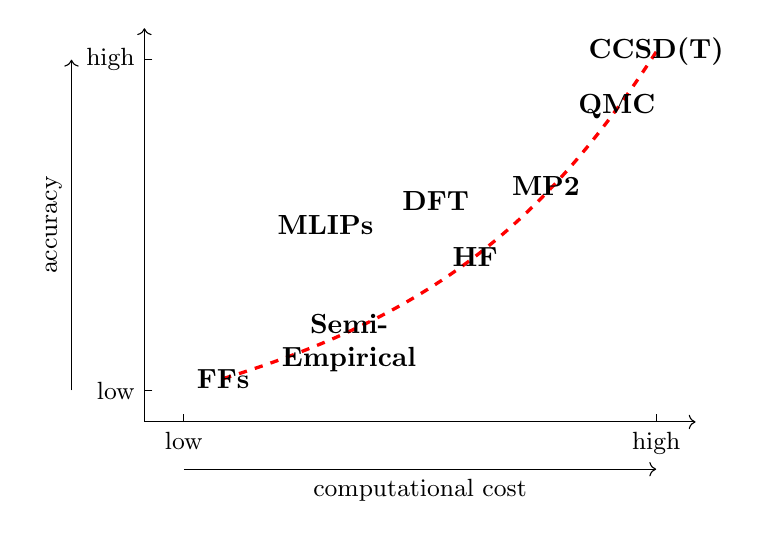
\begin{tikzpicture}
            \draw[->] (0,0)--(7,0);
            \draw[->] (0,0)--(0,5);
            \draw (0.5,0.1)--(0.5,0)node[below]{\small low};
            \draw (6.5,0.1)--(6.5,0)node[below]{\small high};
            \draw[->] (0.5,-0.6)--node[below]{\small computational cost}(6.5,-0.6);
            \draw (0.1,0.4)--(0,0.4)node[left]{\small low};
            \draw (0.1,4.6)--(0,4.6)node[left]{\small high};
            \node[rotate=90] at (-1.1,2.5){
                \tikz{\draw[->] (0.4,0)--node[above]{\small accuracy}(4.6,0);}
            };
            \draw[red,dashed,very thick] (1,0.55) to[bend right=20] (6.5,4.7);
            \node at (1,0.55){\textbf{FFs}};
            \node[align=center] at (2.6,1){\textbf{Semi-}\\ \textbf{Empirical}};
            \node at (4.2,2.1){\textbf{HF}};
            \node at (5.1,3){\textbf{MP2}};
            \node at (6,4){\textbf{QMC}};
            \node at (6.5,4.7){\textbf{CCSD(T)}};
            \node at (2.3,2.5){\textbf{MLIPs}};
            \node at (3.7,2.8){\textbf{DFT}};
        \end{tikzpicture}
        \caption{Quantum Chemistry is a trade-off between accuracy and computational efficiency.}
        \label{computation_trade_off}
    \end{figure}

    Simulations at the atomistic and molecular level can generally be split into two categories:
    \begin{enumerate}[topsep=0pt,label=(\roman*)]
        \item electronic structure methods in which the quantum nature of electrons is taken into account --- these are generally computationally expensive.
        \item classical atomistic approaches in which force fields are used to describe the interactions between atoms --- these are usually computationally cheap.
    \end{enumerate}
    Nowadays the boundaries between the two worlds are blurred and there are a number of approaches at the intersection.
    
    \section{The Schr\"{o}dinger Equation}
    To deal with a molecular system quantum mechanically, we need the Schr\"{o}dinger equation. Let's start with the time-independent Schr\"{o}dinger equation
    \begin{equation}
        \hat{H}\Psi(\vb{r}_1,\dots,\vb{r}_n,\vb{R}_1\dots,\vb{R}_N)=E\Psi(\vb{r}_1,\dots,\vb{r}_n,\vb{R}_1\dots,\vb{R}_N)\,,
    \end{equation}
    where \(\hat{H}\) is the Hamiltonian of the system, \(\Psi\) is the total wavefunction that depends both on the nuclei coordinates \(\{\vb{R}_I\}_{I=1}^{N}\) and the electron coordinates \(\{\vb{r}_i\}_{i=1}^{n}\), and \(E\) is the energy of the system.

    For an isolated molecular system, which is our main interest, the Hamiltonian is given by
    \begin{equation}
        \hat{H}=\hat{T}\n+\hat{T}\e+\hat{V}^{\text{n-n}}+\hat{V}^{\text{n-e}}+\hat{V}^{\text{e-e}}\,,
    \end{equation}
    where
    \begin{itemize}[topsep=0pt]
        \item \(\hat{T}\n\) is the kinetic energy of the nuclei;
        \item \(\hat{T}\e\) is the kinetic energy of the electrons;
        \item \(\hat{V}^{\text{n-n}}\) is the potential energy from nucleus-nucleus repulsion;
        \item \(\hat{V}^{\text{n-e}}\) is the potential energy from nucleus-electron attraction;
        \item \(\hat{V}^{\text{e-e}}\) is the potential energy from electron-electron repulsion.
    \end{itemize}
    We may expand everything out and write
    \begin{align}
        \hat{H}&=\sum_{I=1}^{N}-\frac{\hbar^2}{2M_I}\laplacian_{\vb{R}_I}+\sum_{i=1}^{n}-\frac{\hbar^2}{2m_e}\laplacian_{\vb{r}_i}\notag\\
        &\quad+\sum_{I<J}^{N}\frac{Z_I Z_J e^2}{4\pi\epsilon_0\abs{\vb{R}_I-\vb{R}_J}}-\sum_{I=1}^{N}\sum_{i=1}^{n}\frac{Z_I e^2}{4\pi\epsilon_0\abs{\vb{R}_I-\vb{r}_i}}+\sum_{i<j}^{n}\frac{e^2}{4\pi\epsilon_0\abs{\vb{r}_i-\vb{r}_j}}\,.
    \end{align}

    To avoid writing out so many constants, we introduce the atomic units, in which
    \begin{enumerate}[topsep=0pt,label=(\roman*)]
        \item unit of length is \textit{Bohr} \(a_0\);
        \item unit of charge is the magnitude of the charge on the electron \(e\);
        \item unit of action is \textit{reduced Planck's constant} \(\hbar\);
        \item unit of mass is the mass of the electron \(m_e\).
    \end{enumerate}
    Then
    \begin{equation}
        \hat{H}=\sum_{I=1}^{N}-\frac{1}{2M_I}\laplacian_{\vb{R}_I}+\sum_{i=1}^{n}-\frac{1}{2}\laplacian_{\vb{r}_i}+\sum_{I<J}^{N}\frac{Z_I Z_J}{\abs{\vb{R}_I-\vb{R}_J}}-\sum_{I=1}^{N}\sum_{i=1}^{n}\frac{Z_I}{\abs{\vb{R}_I-\vb{r}_i}}+\sum_{i<j}^{n}\frac{1}{\abs{\vb{r}_i-\vb{r}_j}}\,.
    \end{equation}
    We have a horrible quantum many-body equation to solve! The motions of electrons and nuclei are coupled in a complicated manner, making it impossible to give exact solutions of the Schr\"{o}dinger equation apart from the simplest systems (hydrogen-like atoms), or the limiting case like an infinite `jellium'. We therefore need to make approximations.

    \subsection{Born--Oppenheimer Approximation}
    We will start with a simple but powerful approximation which you have met in Part IB: the \textit{Born--Oppenheimer approximation}.

    The Born--Oppenheimer approximation is based on the fact that the nuclei have masses much greater than the electrons: the proton-to-electron mass ratio is \(m_p/m_e\approx 1836\) and the neutron-to-electron mass ratio is \(m_n/m_e\approx 1839\). Since nuclei are much heavier than electrons, they move much more slowly. Essentially, the Born--Oppenheimer approximation assumes that the fast-moving electrons can adjust instantaneously to the changing positions of the slow-moving nuclei. This is called an \textit{adiabatic approximation}, where the fast electronic degrees of freedom are assumed to adjust instantaneously to the nuclear positions. In practice one often follows the electronic ground-state potential energy surface, so that the electron relaxes to the ground state for each nuclear geometry, although excited-state surfaces can also be considered. An immediate result is that this allows us to decouple the motion of the electrons and nuclei, so we can approximate the total wavefunction as a product of an electronic wavefunction and a nuclear wavefunction:
    \begin{equation}
        \Psi^{\text{B--O}}(\vb{r}_1,\dots,\vb{r}_n,\vb{R}_1\dots,\vb{R}_N)=\Psi\e(\vb{r}_1,\dots,\vb{r}_n;\vb{R}_1\dots,\vb{R}_N)\Psi^{n}(\vb{R}_1\dots,\vb{R}_N)\,.
    \end{equation}
    It is important to note that the electronic wavefunction \(\Psi\e\) is parametrically dependent upon the nuclear coordinates, i.e. they are treated as fixed.
    
    For convenience, we will denote \(\mathsf{r}=(\vb{r}_1,\dots,\vb{r}_n)\) and \(\mathsf{R}=(\vb{R}_1\dots,\vb{R}_N)\).

    Then, for a given set of nuclear geometries, we can write out the electronic Hamiltonian\footnote{There is no clear convention whether \(\hat{V}^{\text{n-n}}(\mathsf{R})\) should appear in the electronic Hamiltonian or in the nuclear Hamiltonian --- but it should definitely appear once, and only once. This is just a constant energy term for each particular nuclear geometry, so it does not affect the solution. But remember to always include it in the potential energy surface (see later).}
    \begin{equation}
        \hat{H}\e(\mathsf{r};\mathsf{R})=\hat{T}\e(\mathsf{r})+\hat{V}^{\text{n-n}}(\mathsf{R})+\hat{V}^{\text{n-e}}(\mathsf{r};\mathsf{R})+\hat{V}^{\text{e-e}}(\mathsf{r})
    \end{equation}
    and solve for the electronic Schr\"{o}dinger equation
    \begin{equation}
        \hat{H}\e(\mathsf{r};\mathsf{R})\Psi\e(\mathsf{r};\mathsf{R})=E\e(\mathsf{R})\Psi\e(\mathsf{r};\mathsf{R})\,.
    \end{equation}
    We may repeat this calculation for a large number of different nuclear geometries and get the electronic energy as a function of the nuclear geometry. This is seen as the average energy of a molecule at a certain nuclear configuration would have, assuming the nuclei are not moving.
    
    The energy we obtained above can be thought of as the potential energy for nuclear motion, and can be combined with the nuclear kinetic energy operator to give the nuclear motion Hamiltonian
    \begin{equation}
        \hat{H}\n(\mathsf{R})=\hat{T}\n(\mathsf{R})+E\e(\mathsf{R})\,.
    \end{equation}
    Solving the Schr\"{o}dinger equation with this Hamiltonian gives the total energy \(E\) and the nuclear wavefunction \(\Psi\n(\mathsf{R})\).

    The Born--Oppenheimer approximation is a foundational approximation used in the vast majority of simulations in computational chemistry. It allows for a computationally tractable approach to molecular systems by significantly reducing the complexity of the coupled electron-nuclei problem. We are now left with only one term in the Hamiltonian that is difficult to deal with, which is the electron-electron repulsion.
    
    
    Born--Oppenheimer approximation works well in most situations where the nuclei move much slower than the electrons. However, it breaks in situations where we have e.g. excited electronic states, conical intersections (where different potential energy surfaces become degenerate and intersect), high energy collisions, certain diffusion processes on metal surfaces.

    \subsubsection{The Potential Energy Surfaces}
    As we pointed out above, since \(E\e(\mathsf{R})\) can be thought of as the potential energy for a given nuclear configuration, a plot of \(E\e\) as a function of the nuclear coordinates \(\mathsf{R}=(\vb{R}_1,\dots,\vb{R}_N)\) is known as a \textit{potential energy surface} (PES).

    However, note that translations and rotations do not affect the electronic energies of a molecular system, so \(E\e\) actually has fewer degrees of freedom than \(\dim\mathsf{R}=3N\). A molecule has \(3\) translational degrees of freedom and \(3\) rotational degrees of freedom (or \(2\) if the molecule is linear), hence a PES is a \(3N-6\) dimensional surface (or \(3N-5\) for linear molecules).

    The PES is crucial in studying chemical reactions, as it allows us to identify transition states (the highest energy points along the reaction pathway) and compute activation energies. These features of the PES help determine how fast a reaction will occur.
    
    Since the Born--Oppenheimer approximation underpins the concept of the PES, PESs are often called Born--Oppenheimer surfaces or Born--Oppenheimer PESs.

    PESs will be covered in more detail in the Part III M4: \textit{Energy Landscapes and Soft Matter} course. We limit our discussion here to key features that are helpful for understanding what comes later in this course.

    \Cref{Fig:landscape} is an example of a (simplified) potential energy surface with key features labeled. The key features include
    \begin{enumerate}[topsep=0pt,label=(\roman*)]
        \item Minima: Local minima on the PES correspond to stable molecular geometries where the molecule has low energy. These are labeled as the Initial State and Final State on \cref{Fig:landscape}. The global minimum represents the most stable structure (the equilibrium geometry) of the system.
        \item Transition States: Saddle points on the PES correspond to transition states, which are higher-energy configurations that the system may pass through during a chemical reaction. These are critical in determining the activation energy required for a reaction to occur.
        \item Energy Barriers: The energy difference between a reactant minimum and a transition state is the activation energy.
        \item The reaction pathway is the route taken
        from reactants to products on the PES. It shows how the nuclei rearrange during a chemical reaction. By following the lowest-energy path (the minimum energy pathway, red line in \cref{Fig:landscape}) between two minima, we can understand how a reaction proceeds.
    \end{enumerate}

    \begin{figure}
        \centering
        \includegraphics[width=0.5\textwidth]{PES.png}
        \caption{A 2-dimensional PES showing the reaction of \(\mathrm{NH_3}\) with \(\mathrm{HCl}\) to produce \(\mathrm{NH_4^+}\) and \(\mathrm{Cl^-}\). Figure adapted from the official course notes by Prof. Angelos Michaelides.}
        \label{Fig:landscape}
    \end{figure}

    One limitation of PESs is that for systems with a large number of atoms, the PES becomes a high-dimensional object that is difficult to visualize or compute.

    \section{Types of Simulations}
    We will now briefly explain the various types of simulations in quantum chemistry.
    \begin{enumerate}[topsep=0pt,label=(\roman*)]
        \item Single point calculations: It calculates the energy of a molecule at a particular nuclear configuration. This corresponds to computing a single, fixed point on a PES.
        \item Geometry optimisation: it finds the most stable structure of a molecule with the nuclear positions giving the lowest energy. During optimization, the molecular geometry is iteratively refined by minimising the total energy of the system, which is typically done by
        calculating the forces acting on each atom, given by
        \begin{equation}
            \vb{F}_I=-\pdv{V_{\text{PES}}(\mathsf{R})}{\vb{R}_I}\,.
        \end{equation}
        The nuclear positions are adjusted until the forces on all atoms are (sufficiently close to) zero. The result corresponds to a local/global minimum of the PES.
        \item Molecular dynamics (MD): it simulates the time evolution of a system consisting of interacting atoms/molecules. It may either be done completely classically or quantum mechanically. The nuclei may also be treated quantum mechanically in \textit{path integral molecular dynamics} (PIMD) using the path integral formulation of quantum mechanics by Feynman. 
        \item Monte Carlo (MC): it is a class of stochastic algorithms used to model systems by randomly sampling possible configurations according to a probability distribution, often related to the system's energy. It focuses on exploring the configurational space of a system to estimate properties such as thermodynamic averages or equilibrium distributions.
    \end{enumerate}

    Finally, we note that in doing simulations we have a choice about whether to treat the electrons/nuclei classically or quantum mechanically. The vast majority of simulations in computational chemistry involve classical nuclei. Simulations with quantum nuclei are much less common, but quantum nuclear effects like tunneling and zero-point energy can be significant on light elements like hydrogen.

    \begin{figure}
        \centering
        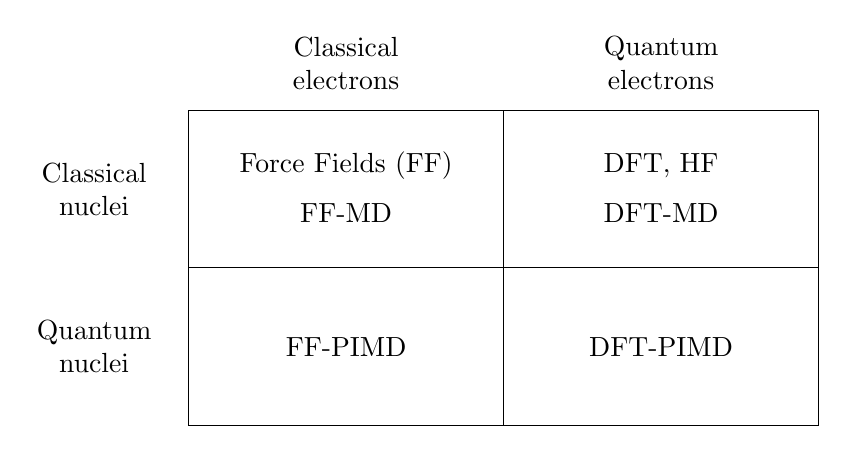
\begin{tikzpicture}
            \draw (0,0) rectangle (8,4);
            \draw (0,2)--(8,2);
            \draw (4,0)--(4,4);
            \node[align=center] at (2,4.6) {Classical \\ electrons};
            \node[align=center] at (6,4.6) {Quantum \\ electrons};
            \node[align=center] at (-1.2,1) {Quantum \\ nuclei};
            \node[align=center] at (-1.2,3) {Classical \\ nuclei};
            \node at (2,1) {FF-PIMD};
            \node at (6,1) {DFT-PIMD};
            \node at (2,3.3) {Force Fields (FF)};
            \node at (2,2.7) {FF-MD};
            \node at (6,3.3) {DFT, HF};
            \node at (6,2.7) {DFT-MD};
        \end{tikzpicture}
        \caption{simplified categorisation of some broad classes of simulation techniques in theoretical chemistry.}
    \end{figure}

    \section{Force Fields}
    \subsection{Traditional Force Fields}
    Schr\"{o}dinger equations for molecular systems are infamously hard to solve, so a genius idea would be discarding them and going back to Newton's classical mechanics.

    \textit{Force field} (FF) methods neglect the electrons as well as the quantum mechanical nature of molecules, and calculate the energies of chemical systems using empirical potentials.

    A familiar example is the \textit{Morse potential}, which is often used to model the interaction
    between a pair of atoms in a diatomic molecule. It has the form
    \begin{equation}
        V(r)=D_e\left(1-\ee^{-\beta(r-r_e)}\right)^2\,.
    \end{equation}
    Comments (that should be familiar from IB):
    \begin{enumerate}[topsep=0pt,label=(\roman*)]
        \item \(D_e\) is the dissociation energy, i.e. \(D_e=\lim_{r\to\infty}V(r)\).
        \item The minimum of \(V(r)\) occurs at \(r=r_e\), the equilibrium bond length.
        \item \(\beta\) controls the width of the potential, which is related to the stiffness of the bond.
        \item The potential is anharmonic: it is steeper for compression (\(r<r_e\)) than for stretching (\(r>r_e\)). The potential is approximately harmonic near the equilibrium point (from Taylor expansion).
    \end{enumerate}

    Another example is the \textit{Lennard-Jones potential}, which is used to describe the intermolecular interaction between a pair of neutral atoms or molecules. It has the expression
    \begin{equation}
        V(r)=4\epsilon\left[\left(\frac{\sigma}{r}\right)^{12}-\left(\frac{\sigma}{r}\right)^6\right]\,.
    \end{equation}
    Comments (that should be familiar from IB):
    \begin{enumerate}[topsep=0pt,label=(\roman*)]
        \item \(\epsilon\) is the depth of the potential well.
        \item \(\sigma\) is the zero point of the potential.
        \item The \((\sigma/r)^6\) term represents the long-ranged attractive van der Waals interaction.
        \item The \((\sigma/r)^{12}\) term represents the strong repulsive interaction at short distances due to Pauli repulsion. The choice of the power 12 here is arbitrary --- it's just for computational convenience while making sure that it dominates over the \((\sigma/r)^6\) term at short distances. A more physically motivated form replaces this with an exponential (the exp-6 or Buckingham potential).
    \end{enumerate}

    To describe more complicated molecules, more complicated potentials have been developed. It's common to refer to these as \textit{molecular mechanics potentials}. Examples of these include widely used force fields such as AMBER, CHARMM, and OPLS. A generic energy expression for potentials of this type can be written as
    \begin{equation}
        E_{\text{total}}=E_{\text{stretch}}+E_{\text{bend}}+E_{\text{torsion}}+E_{\text{non-bonded}}\,.
    \end{equation}
    Some of the simplest possible forms of these potentials might be
    \begin{itemize}[topsep=0pt]
        \item Bond stretching energy: This may be modeled by a harmonic potential
        \begin{equation}
            E_{\text{stretch}}=\sum_{\text{bonds}}k_b(r-r_e)^2\,.
        \end{equation}
        \item Angle bending energy: This is the energy due to deviation from equilibrium bond angles, which can also be modeled by a harmonic potential
        \begin{equation}
            E_{\text{bend}}=\sum_{\text{angles}}k_\theta(\theta-\theta_e)^2\,.
        \end{equation}
        \item Torsional (dihedral) energy: This is the energy associated with rotation around bonds, typically modeled using a periodic potential function
        \begin{equation}
            E_{\text{torsion}}=\sum_{\text{dihedrals}}\frac{V_n}{2}[1+\cos(n\phi-\gamma)]\,,
        \end{equation}
        where \(n\) is the periodicity of the torsion and \(\gamma\) is the phase offset.
        \item Non-bonded interaction energies: this includes the van der Waals energy, which may be modeled using the Lennard-Jones potential
        \begin{equation}
            E_{\text{vdW}}=\sum_{\text{non-bonded}}4\epsilon\left[\left(\frac{\sigma}{r}\right)^{12}-\left(\frac{\sigma}{r}\right)^6\right]\,,
        \end{equation}
        and the electrostatic energy, which is computed by Coulomb's law
        \begin{equation}
            E_{\text{electrostatic}}=\sum_{\text{non-bonded}}\frac{q_iq_j}{4\pi\epsilon_0 r_{ij}}\,.
        \end{equation}
    \end{itemize}

    The advantages of the force field methods include
    \begin{itemize}[topsep=0pt]
        \item Fast and has good computational scaling \(O(n)\), meaning that computational time scales with \(n\), the number of atoms in the system. For comparison, the scaling of quantum methods: DFT is \(O(n^3)\) and CCSD(T) is \(O(n^7)\).
        \item Can be accurate, if the system is inside the space the force field is parameterised.
        \item Tuning parameters can give insight.
        \item Simple and easy to use (once a model is developed).
    \end{itemize}
    Disadvantages include
    \begin{itemize}[topsep=0pt]
        \item Not accurate outside training space.
        \item Generally not good for reactions.
        \item No electrons (most are not
        polarisable).
        \item Difficult and labour-intensive to parameterise --- tons of parameters need to be fitted.
        \item Struggle for complex systems and interfaces.
        \item Functional forms can be too restrictive.
    \end{itemize}

    \subsection{Machine Learning Force Fields}
    You may have noticed that machine learning (ML) has become phenomenal in society over the last few years. It has also had a huge impact in the physical sciences, including chemistry, winning two Nobel prizes in 2024.

    Here we discuss a new class of force fields that are commonly referred to as \textit{machine learning interatomic potentials} (MLIPs). MLIPs is a rapidly evolving field at the frontier of theoretical chemistry, delivering the accuracy of \textit{ab initio}/electronic structure methods at a cost more typical of force fields.

    We will only give a quick overview of MLIPs. You will learn more about it in Part III L10 course.

    The generation of accurate MLIPs relies heavily on large amounts of high quality data against which the potentials are parameterised. The most common current approach for the generation of MLIPs is outlined here as the following sequence of steps
    \begin{enumerate}[topsep=0pt,label=(\roman*)]
        \item Assemble a set of reference points that serve as training data for the properties we seek to learn: in the current context it is the multi-dimensional PES that we are aiming to learn.
        \item Represent the training data in terms of atomic environments using appropriate ``descriptors''. This is sort of translating the dataset into something that a machine can understand and fit.
        \item Train the machine learning model.
        \item Test, validate, and if necessary iteratively improve the MLIP.
    \end{enumerate}
    Then the MLIP is ready to be applied.

    Here we will briefly introduce two types of MLIPs:
    \begin{enumerate}[topsep=0pt,label=(\roman*)]
        \item \textit{Behler--Parrinello Neural Network Potentials} (NNPs): It uses neural networks to predict the potential energy of a system by summing up contributions from each atom. These atomic contributions depend on the local environment of each atom. As the descriptor to describe the local environment they use so-called atom-centered symmetry functions. These descriptors capture information about the local environment of the atom: e.g. distances and angles between neighboring atoms, and they are invariant to rotations, translations, and the permutation of atoms. The total energy of the system is the sum of the individual atomic energies predicted by the neural network.
        \item \textit{Gaussian Approximation Potentials} (GAP): It models the potential energy surface using the smooth overlap of atomic positions (SOAP) descriptor to represent the local atomic environment. SOAP describes the distribution of neighboring atoms around a central atom in a way that is invariant to rotations.
    \end{enumerate}

    \section{Density Functional Theory}
    Rather than stepping back to classical mechanics, what else can we do to avoid solving the horrible looking Schr\"{o}dinger equation
    \begin{equation}
        \hat{H}\Psi(\vb{r}_1,\dots,\vb{r}_n,\vb{R}_1\dots,\vb{R}_N)=E\Psi(\vb{r}_1,\dots,\vb{r}_n,\vb{R}_1\dots,\vb{R}_N)
    \end{equation}
    while preserving the quantum mechanical nature of molecular systems?

    The answer is, rather than looking at the molecular wavefunction \(\Psi:\RR^{3(N+n)}\to\CC\) of \(3(N+n)\) variables, we look at the electron density \(n:\RR^3\to\RR\), an apparently lower dimensional and so simpler object. This leads to the \textit{density functional theory} (DFT).\footnote{A more mathematical treatment of DFT can be found in my notes on \textit{B10: Electronic Structure}. Pathetically, this part of the course is now removed, so you can't see it in the official course notes.}

    Before introducing density functional theory, let's first introduce what a \textit{functional} is. Abstractly, let \(V\) be a vector space over a field \(\FF\), then a \textit{functional} is a map \(F:V\to\FF\). Within our context, we can think of a functional as special type of function whose input is a function, and the output is a number. For example, \(\max_{x\in\RR}\) is a functional, giving \(\max_{x\in\RR}[\sin x]=1\), \(\max_{x\in\RR}[4-x^2]=4\) etc. A particularly important class of functionals is definite integrals, such as
    \begin{equation}
        F[f]=\int_{\alpha}^{\beta}\dd{x}f(x)
    \end{equation}
    for some \(\alpha,\beta\). Note that it is conventional to put the argument of a functional in square brackets \([\ \ ]\).

    \subsection{The Hohenberg--Kohn Theorems}
    \subsubsection{The First Hohenberg--Kohn Theorem}
    The essence of density functional theory is that the ground state electron energy is a unique functional of the ground state electron density. This means that given a ground state electron density \(n(\vb{r})\), then we know which external potential (generated by the nuclei under Born--Oppenheimer approximation) uniques produces it, and then we know the unique electron wavefunction it corresponds to, and also the ground state electron energy, and everything else.

    This is known as the First Hohenberg--Kohn theorem.

    \begin{thm}[The first Hohenberg--Kohn theorem]
        The external potential \(V_{\text{ext}}(\vb{r})\) and hence the total energy are unique functionals of the electron density \(n(\vb{r})\) up to an additive constant.
    \end{thm}
    \begin{proof}
        Suppose there are two external potentials \(V_{1}(\vb{r})\) and \(V_{2}(\vb{r})\) both lead to the same \(n(\vb{r})\). There will be two Hamiltonians \(\hat{H}_1\) and \(\hat{H}_2\) with the same ground state density, but different wavefunctions \(\Psi_1\) and \(\Psi_2\). Now use the variational principle,
        \begin{align}
            E_1^0<\mel{\Psi_2}{\hat{H}_1}{\Psi_2}&=\mel{\Psi_2}{\hat{H}_2}{\Psi_2}+\mel{\Psi_2}{\hat{H}_2-\hat{H}_1}{\Psi_2}\notag\\
            &=E_2^0+\int\dd[3]{\vb{r}}n(\vb{r})[V_1(\vb{r})-V_2(\vb{r})]\,,
        \end{align}
        where \(E_0^1\) and \(E_2^0\) are the ground state energies for \(\hat{H}_1\) and \(\hat{H}_2\), respectively. The subscripts 1 and 2 may be interchanged to give a second inequality. These two inequalities may be added to give
        \begin{equation}
            E_1^0+E_2^0<E_2^0+E_1^0\,,
        \end{equation}
        which is a contradiction.\qed
    \end{proof}

    Thus, at least in principle, the ground-state density determines (within a constant) the external potential in the Schr\"{o}dinger equation of which it is a solution. Therefore, the electronic energy is also uniquely determined, via
    \begin{align}
        E\e[n]&=\expval{\hat{T}\e+\hat{V}^{\text{n-e}}[n]+\hat{V}^{\text{e-e}}}{\Psi[n]}\notag\\
        &=T\e[n]+V^{\text{n-e}}[n]+V^{\text{e-e}}[n]\notag\\
        &=T\e[n]+V^{\text{e-e}}[n]+\int\dd[3]{\vb{r}} \tilde{V}_{\text{ext}}[n](\vb{r})n(\vb{r})\,,
    \end{align}
    where \(\Psi[n]\) and \(\tilde{V}_{\text{ext}}[n](\vb{r})\) are the wavefunction and the external potential determined by \(n(\vb{r})\).

    \subsubsection{The Second Hohenberg--Kohn theorem}

    The First Hohenberg--Kohn theorem shows that working with electron density is theoretically possible, however, the form of \(E\e[n]\) it gives is troublesome: the \(\tilde{V}_{\text{ext}}[n](\vb{r})\) depends on the electron density. Rather, in a real problem, under Born--Oppenheimer approximation, we have a specific nuclear arrangement and hence a known potential, and we want to find a optimum electron density. This is realised by the second Hohenberg--Kohn theorem.

    We introduce the shorthand notation
    \begin{equation}
        F[n]=\mel{\Psi}{\hat{F}}{\Psi}=\mel{\Psi}{\hat{T}+\hat{V}^{\text{e-e}}}{\Psi}=T[n]+V^{\text{e-e}}[n]\,.
    \end{equation}
    Now an energy functional for an \textbf{arbitrary external potential} \(V_{\text{ext}}(\vb{r})\) unrelated to the \(\tilde{V}_{\text{ext}}(\vb{r})\) determined by \(n(\vb{r})\) can be defined:
    \begin{equation}
        E_V[n]=F[n]+\int\dd[3]{\vb{r}}V_{\text{ext}}(\vb{r})n(\vb{r})\,.
    \end{equation}

    \begin{thm}[The second Hohenberg--Kohn theorem]
        For an arbitrary external potential \(V_{\text{ext}}\) and electron densities \(n(\vb{r})\) of \(N\) electrons,
        \begin{equation}\label{DFT_energy}
            E_V[n]=F[n]+\int\dd[3]{\vb{r}}V_{\text{ext}}(\vb{r})n(\vb{r})\ge E_0\,,
        \end{equation}
        where \(E_0\) is the ground state energy for \(N\) electrons in the external potential \(V_{\text{ext}}(\vb{r})\), and this functional reaches its minimum if and only if \(n\) is the true ground state electron density in such external potential \(V_{\text{ext}}\).
    \end{thm}
    \begin{proof}
        By the first theorem, a given \(n(\vb{r})\) determines its own external potential \(\tilde{V}_{\text{ext}}(\vb{r})\) and ground state \(\ket{\tilde{\Psi}}\). If this state is used as a trial state for the Hamiltonian with external potential \(V_{\text{ext}}(\vb{r})\), we have
        \begin{equation}
            \expval{\hat{H}}{\tilde{\Psi}}=\expval{\hat{F}}{\tilde{\Psi}}+\expval{\hat{V}_{\text{ext}}}{\tilde{\Psi}}=F[n]+\int\dd[3]{\vb{r}}V_{\text{ext}}(\vb{r})n(\vb{r})=E_V[n]\ge E_0
        \end{equation}
        by the variational principle. For non-degenerate ground states, equality holds if \(\ket{\tilde{\Psi}}\) is the ground state for the potential \(V_{\text{ext}}(\vb{r})\).\qed
    \end{proof}

    This means that to find the true ground state energy of a molecular system, we only need to find the electron density \(n(\vb{r})\) that minimises the functional \(E_V[n]\)!

    \subsection{Kohn--Sham Theory}
    Using the Hohenberg--Kohn theorems, we have reformulated the Schr\"{o}dinger equation, i.e. finding \(\Psi\) that minimises
    \begin{equation}
        \expval{\hat{T}\e+\hat{V}^{\text{n-e}}+\hat{V}^{\text{e-e}}}{\Psi}\,,
    \end{equation}
    to finding the electron density \(n\) that minimises the energy functional
    \begin{equation}
        E_V[n]=T\e[n]+V^{\text{e-e}}[n]+\int\dd[3]{\vb{r}}V_{\text{ext}}(\vb{r})n(\vb{r})\,,
    \end{equation}
    which should be much simpler as \(n\) is a lower dimensional object.

    This now seems like an easy problem as long as we know what the functionals \(T\e[n]\) and \(V^{\text{e-e}}[n]\) are --- but we don't. We haven't changed the nature that this is a quantum many-body problem. The complicated correlated motions of the electrons made it impossible to give their kinetic and interaction energy in a simple closed form. To make progress, we need Kohn--Sham theory.

    Although we don't know the kinetic energy of correlated electrons, we know the kinetic energy of a single electron with wavefunction \(\psi\), which is
    \begin{equation}
       -\frac{1}{2} \int\dd[3]{\vb{r}}\psi^*(\vb{r})\laplacian\psi(\vb{r})\,.
    \end{equation}
    Hence, if we assume that the electrons are moving in their orbitals \(\{\phi_i\}\) without interacting with each other\footnote{Recall that orbitals are effective one-electron wavefunctions. Kohn--Sham theory essentially assumes the system to have a non-interacting wavefunction as a Slater determinant made from the Kohn--Sham orbitals.}, we have the kinetic energy
    \begin{equation}
        T_s\e[n]=-\frac{1}{2}\sum_i\int\dd[3]{\vb{r}}\phi_i^*(\vb{r})\laplacian\phi_i(\vb{r})\,.
    \end{equation}
    These \(\{\phi_i\}\) are known as the \textit{Kohn--Sham orbitals}. \(T_s\e[n]\) is the kinetic energy functional of non-interacting electrons of density \(n\), where the subscript \(s\) indicates ``single-particle'' electrons.

    We also don't know the potential energy from electron interaction due to exchange interactions and correlations\footnote{Correlation basically means that an electronic system can lower its energy by letting its electrons to avoid each other, so the motion of the electrons are ``correlated''. See more in later chapters on Hartree--Fock theory.}. However, we are very familiar with the Coulomb interaction energy of the electrons. This contribution is known as the \textit{Hartree energy} and has the simple form
    \begin{equation}
        E^{\text{Hartree}}[n]=\frac{1}{2}\int\dd[3]{\vb{r}}\dd[3]{\vb{r}'}\frac{n(\vb{r})n(\vb{r}')}{\abs{\vb{r}-\vb{r}'}}.
    \end{equation}

    Hence, by pulling these two contributions out, we obtain the formula
    \begin{align}
        E_V[n]&=T\e[n]+V^{\text{e-e}}[n]+V^{\text{n-e}}[n]\notag\\
        &=T_s\e[n]+E^{\text{Hartree}}[n]+V^{\text{n-e}}[n]+\left(T\e[n]+V^{\text{e-e}}[n]-T_s\e[n]-E^{\text{Hartree}}[n]\right)\notag\\
        &=T_s\e[n]+E^{\text{Hartree}}[n]+V^{\text{n-e}}[n]+E^{\text{xc}}[n]\,,
    \end{align}
    where
    \begin{equation}
        E^{\text{xc}}[n]\coloneqq T\e[n]+V^{\text{e-e}}[n]-T_s\e[n]-E^{\text{Hartree}}[n]
    \end{equation}
    is the exchange and correlation energy. This is now the only term that is unknown. All the complicated quantum-mechanical many-body effects are placed in this term only.

    Recall when we introduced the Kohn--Sham orbitals, we defined them as the ``effective non-interacting one-electron orbitals''. In order to solve them, we need to solve their Schr\"{o}dinger equation. The effective potential that the electron is moving is
    \begin{align}
        V^{\text{eff}}(\vb{r})&=\frac{\delta(E^{\text{Hartree}}[n]+V^{\text{n-e}}[n]+E^{\text{xc}}[n])}{\delta n(\vb{r})}\notag\\
        &=\int\dd[3]{\vb{r}'}\frac{n(\vb{r}')}{\abs{\vb{r}-\vb{r}'}}+V_{\text{ext}}(\vb{r})+\frac{\delta E^{\text{xc}}[n]}{\delta n(\vb{r})}\notag\\
        &\eqqcolon V^{\text{Hartree}}(\vb{r})+V_{\text{ext}}(\vb{r})+V^{\text{xc}}(\vb{r})\,,
    \end{align}
    so the Kohn--Sham orbitals are solved from the Schr\"{o}dinger equation
    \begin{equation}
        \left[-\frac{1}{2}\laplacian+V^{\text{eff}}\right]\phi_i(\vb{r})=\epsilon_i\phi_i(\vb{r})\,.
    \end{equation}
    This is a single electron Schr\"{o}dinger equation so it is not painful to solve.

    As you can see, the electron density for minimum energy depends on the energy functional, which depends on the Kohn--Sham orbitals, which depends on the effective potentials, which in turn depends on the electron density. Thus, we need to perform this in an iterative process. We must have an initial guess on the electron density \(n(\vb{r})\), work everything out, and determine a new electron density \(n(\vb{r})\), and repeat until the electron density \(n(\vb{r})\) converges. This is known as a \textit{self-consistent field} (SCF) method. A flow chart is shown in \cref{Fig:SCF}.
    
    \begin{figure}
        \centering
        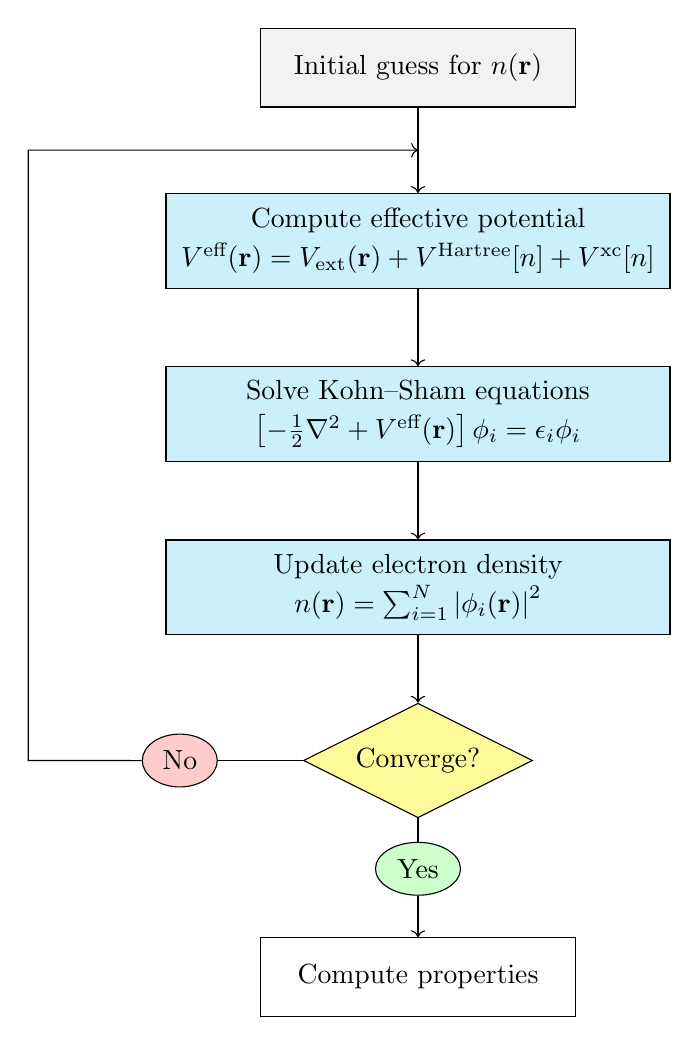
\begin{tikzpicture}[scale=1.1]
            \node at (0,4.5) (A) [draw,fill=gray!10,minimum height=1cm,minimum width=4cm] {Initial guess for \(n(\vb{r})\)};
            \node at (0,2.5) (B) [align=center,draw,fill=cyan!20,minimum height=1.2cm,minimum width=6.4cm] {Compute effective potential \\[2pt] \(V^{\text{eff}}(\vb{r})=V_{\text{ext}}(\vb{r})+V^{\text{Hartree}}[n]+V^{\text{xc}}[n]\)};
            \draw[->] (A.south)--node(M){}(B.north);
            \node at (0,0.5) (C) [align=center,draw,fill=cyan!20,minimum height=1.2cm,minimum width=6.4cm] {Solve Kohn--Sham equations \\[2pt] \(\left[-\frac{1}{2}\laplacian+V^{\text{eff}}(\vb{r})\right]\phi_i=\epsilon_i\phi_i\)};
            \draw[->] (B.south)--(C.north);
            \node at (0,-1.5) (D) [align=center,draw,fill=cyan!20,minimum height=1.2cm,minimum width=6.4cm] {Update electron density \\[2pt] \(n(\vb{r})=\sum_{i=1}^{N}\abs{\phi_i(\vb{r})}^2\)};
            \draw[->] (C.south)--(D.north);
            \node at (0,-3.5) (E) [draw,fill=yellow!40,shape aspect=2,diamond] {Converge?};
            \draw[->] (D.south)--(E.north);
            \node at (-2.75,-3.5) (H) [draw,fill=red!20,shape aspect=1.7,ellipse] {No};
            \draw (E.west)--(H.east);
            \draw[<-] (M.center)--++(-4.5,0)--(-4.5,-3.5)--(H.west);
            \node at (0,-4.75) (F) [draw,fill=green!20,shape aspect=1.7,ellipse] {Yes};
            \draw (E.south)--(F.north);
            \node at (0,-6) (G) [draw,minimum height=1cm,minimum width=4cm] {Compute properties};
            \draw[->] (F.south)--(G.north);
        \end{tikzpicture}
        \caption{Illustration of the self-consistent field (SCF) cycle used to solve the Kohn--Sham equations and obtain the ground state density and total energy.}
        \label{Fig:SCF}
    \end{figure}

    \subsection{Exchange and Correlation}
    As we commented above, all the complexity of Kohn--Sham theory lies in the exchange correlation functional, where all the quantum many-body effects live in. It is impossible to give an exact and closed form expression of this functional, so approximations must be made.

    As its name suggests, \(E^{\text{xc}}[n]\) have two contributions
    \begin{enumerate}[topsep=0pt,label=(\roman*)]
        \item Electron exchange: this arises because a many-body wavefunction must by antisymmetric under exchange of any two electrons since electrons are fermions. This leads to the Pauli exclusion principle, which reduces the probability of electrons with the same spin coming close to each other, and therefore reduces the Coulomb repulsion.
        \item Electron correlation: it also reduces the Coulomb energy between electrons because the motion of each individual electron is correlated with the motion of all others, helping electrons to keep spatially separated.
    \end{enumerate}

    Note that an important consequence of exchange interaction being approximated is that it leads to \textit{self-interaction error}, i.e. an electron is repelling itself. In theories like Hartree--Fock where electron exchange are exact, the self repulsion in the Coulomb term is precisely cancelled by the self exchange in the exchange term, so there is no self-interaction. However in DFT, the Coulomb term (Hartree energy) is exact, while the exchange term is not, so the self-interaction is not completely cancelled. This significantly affects the accuracy of DFT for systems with strongly correlated electrons or localised electrons (e.g. transition metal complexes). More errors in DFT will be introduced in later sections.

    An exchange correlation functional can be classified as being either ``empirical'' or ``non-empirical''. An empirical functional aims to reproduce experiment results and usually contain a lot of parameters fitted from experimental data. A non-empirical functional is designed to abide by a number of physical constraints which the exact \(E^{\text{xc}}\) functional should obey and do not include parameters other than the fundamental constants.

    A major way of categorising exchange correlation functional is to group them in terms of their physical complexity, and it is known as the \textit{Jacob's ladder}. As you climb up the ladder, the functional gets more complex and computationally more expensive, but will usually give higher accuracy. The five rungs of the Jacob's ladder, from low to high, are
    \begin{enumerate}[topsep=0pt,label=(\roman*)]
        \item local density approximation (LDA);
        \item generalised gradient approximation (GGA);
        \item meta-GGA;
        \item hybrid functionals;
        \item double-hybrid functionals.
    \end{enumerate}

    \subsubsection{Local Density Approximation}
    There is a system in which the exchange energy is known exactly, which is the \textit{uniform electron gas} (a ``jellium''). A uniform electron gas with constant electron density \(n\) has the exchange energy
    \begin{equation}
        E^{\text{x-UEG}}[n]=-\frac{3}{4}\left(\frac{3}{\pi}\right)^{\frac{1}{3}}\int\dd[3]{\vb{r}} n^{4/3}\,.
    \end{equation}
    There are also some widely accepted expressions for the correlation energy in uniform electron gas, but they are significantly more complicated. It has the general form
    \begin{equation}
        E^{\text{c-UEG}}[n]=\int\dd[3]{\vb{r}} n \epsilon^{\text{c-UEG}}(n)
    \end{equation}
    for some function \(\epsilon^{\text{c-UEG}}\).

    Knowing this, a natural thought of approximating the exchange and correlation energy in a general system is to treat each point locally as uniform electron gas, so that
    \begin{equation}
        E^{\text{xc-LDA}}[n]=\int\dd[3]{\vb{r}} n(\vb{r})\epsilon^{\text{xc-LDA}}(n(\vb{r}))\,,
    \end{equation}
    where \(\epsilon^{\text{xc-LDA}}\) is the exchange-correlation energy per particle of the homogeneous electron gas of density \(n\). From our expressions for uniform electron gas, it should be
    \begin{align}
        \epsilon^{\text{xc-LDA}}(n(\vb{r}))&=\epsilon^{\text{x-LDA}}+\epsilon^{\text{c-LDA}}\notag\\
        &=-\frac{3}{4}\left(\frac{3}{\pi}\right)^{\frac{1}{3}}n^{1/3}(\vb{r})+\epsilon^{\text{c-UEG}}(n(\vb{r}))\,.
    \end{align}
    This is called \textit{local density approximation} (LDA).

    Strictly, the LDA is valid only for slowly varying densities. However, experience with calculations of atoms, molecules, and solids shows that the LDA actually works surprisingly well, given its crudeness.

    \subsubsection{Generalised Gradient Approximation}
    To go beyond LDA, a natural thought is to include the local gradient of the electron density, in addition to the electron density itself, into the exchange correlation energy expression. Hence, this is known as \textit{generalised gradient approximation} (GGA). It has the general form
    \begin{equation}
        E^{\text{xc-GGA}}[n]=\int\dd[3]{\vb{r}}n(\vb{r})\epsilon^{\text{xc-GGA}}(n(\vb{r}),\grad n(\vb{r}))\,.
    \end{equation}

    Since it is extremely difficult to come up with a valid correlation functional, there is an extremely limited number of them. Hence, the main difference between the GGAs is usually found in the exchange energy density terms. Since the GGA should reduce to LDA when \(\abs{\grad n}=0\), a lot of GGA exchange functionals can be written as a series expansion
    \begin{equation}
        \epsilon^{\text{x-GGA}}(n,s)=\epsilon^{\text{x-LDA}}F^{\text{x-GGA}}(s)\,,
    \end{equation}
    where \(F^{\text{x-GGA}}(s)\) is known as the \textit{enhancement factor} and \(s=\abs{\grad n}/2(3\pi^2)^{1/3}n^{4/3}\) is a dimensionless reduced density gradient.

    \begin{ex}
        Two related GGA functionals PBE and revPBE have the enhancement factor
        \begin{equation}
            F^{\text{x-PBE}}=1+\kappa-\frac{\kappa}{1+\frac{\mu s^2}{\kappa}}\,,
        \end{equation}
        where \(\mu\) is some parameter that is the same for PBE and revPBE. The difference is only in the parameter \(\kappa\): \(\kappa^{\text{revPBE}}=1.245\) while \(\kappa^{\text{PBE}}=0.804\). This makes \(F_x\) rise more rapidly with \(s\) for revPBE than for PBE. As a consequence, regions with large reduced density gradients are stabilised more with revPBE than PBE. This means that in a revPBE calculation, a rapid reduction of the electron density in the internuclear region is expected, which in turn leads to weaker interactions with revPBE.
        \begin{figure}
            \centering
            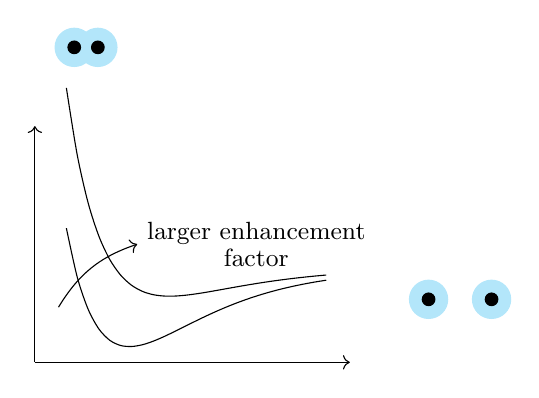
\begin{tikzpicture}
                \draw[->] (0,0)--(4,0);
                \draw[->] (0,0)--(0,3);
                \draw[domain=-0.8:2.5, smooth, variable=\x] plot ({\x+1.2}, {0.2+(1-2.72^(-\x))^2});
                \draw[domain=-0.8:2.5, smooth, variable=\x] plot ({\x+1.2}, {0.6+0.6*(1-2.72^(-\x))^2+0.4*2.72^(-2*\x)});
                \draw[->] (0.3,0.7) to[bend left=20] (1.3,1.5)node[right,align=center]{\small larger enhancement \\[-2pt] \small factor};
                \fill[cyan!30] (5,0.8) circle (0.25);
                \fill[cyan!30] (5.8,0.8) circle (0.25);
                \draw[fill=black] (5,0.8) circle (0.08);
                \draw[fill=black] (5.8,0.8) circle (0.08);
                \fill[cyan!30] (0.5,4) circle (0.25);
                \fill[cyan!30] (0.8,4) circle (0.25);
                \draw[fill=black] (0.5,4) circle (0.08);
                \draw[fill=black] (0.8,4) circle (0.08);
            \end{tikzpicture}
            \caption{GGA with high enhancement factors encourage regions with high local gradient densities. Therefore they predict weaker binding.}
        \end{figure}
    \end{ex}

    DFT only became widely used in quantum chemistry after GGAs were developed. It generally has a significant improvement in accuracy compared with LDA, while it does not increase the computational costs significantly.

    \subsubsection{Meta-GGAs}
    Having included the local electron density gradients in GGAs, we can further include the second order terms such as the second derivative of electron density \(\laplacian n(\vb{r})\), and/or kinetic energy densities \(\tau_\sigma(n)=\frac{1}{2}\sum_i\abs{\grad\phi_i}^2\). These are known as \textit{meta-GGAs}.

    \subsubsection{Hybrid Functionals}
    The \textit{hybrid functionals} (or \textit{hybrid GGA}) add the exact exchange interaction calculated from Hartree--Fock (HF) theory to some conventional treatment of DFT exchange and correlation via a technique called adiabatic connection\footnote{Detail in my course notes on B10 electronic structure.}.

    For example, the most widely used functional in quantum chemistry, B3LYP, takes the following form
    \begin{equation}
        E^{\text{xc}}=E^{\text{xc-GGA}}+a(E^{\text{x-HF}}-E^{\text{x-GGA}})\,.
    \end{equation}

    Hybrid functionals have significantly better accuracy, along with a significantly longer computation time. Hybrid functionals are so successful because they benefit from error compensation between ``underbinding'' of (meta-)GGAs and the ``overbinding'' of Hartree--Fock. The underbinding of GGAs is due to the self-interaction error and the overbinding of HF is due to the lack of correlation.

    \subsubsection{Double-hybrid Functionals}
    Double-hybrid functionals incorporate virtual (unoccupied) orbitals into the functional. For example, the B2-PLYP functional has the form
    \begin{equation}
        E^{\text{xc}}=(1-a_x)E^{\text{x-DFT}}+a_x E^{\text{x-HF}}+(1-a_c)E^{\text{c-DFT}}+a_c E^{\text{c-PT2}}\,.
    \end{equation}
    It can be seen that in addition to exact exchange (via HF), electron correlation is taken into account through perturbation theory (PT).

    These functionals are very computationally expensive and are still not as widely used as other functionals.

    \subsection{Dispersion Forces in DFT}
    Another serious problem found for functionals on the first four rungs of Jacob's ladder is that they fail to account for van der Waals dispersion forces. This greatly limited the use of DFT in areas such as biology. Since this century, considerable progress has been made to correct this dispersion error.
    \subsubsection{Dispersion Force}
    The concept of dispersion forces should be familiar. It originates from the electrostatic attraction between the instantaneous dipole in one particle arising from electron density fluctuation and the induced dipole on another particle.

    It is hard for DFT to account for dispersion forces because
    \begin{enumerate}[topsep=0pt,label=(\roman*)]
        \item Under Kohn--Sham approximation, the DFT is a mean field theory, in which an electron interacts with the total electron density, rather than with instantaneous electron positions which is the basis of the dispersion interaction.
        \item Most exchange correlation functionals used are local. They only use information about the local electron density at a single point, so there is no way electrons on one molecule know there are instantaneous dipole produced on another molecule.
    \end{enumerate}

    This means that for two noble gas atoms, for example, these functionals can give binding or repulsion only when there is an overlap of the electron densities of the two atoms.

    \begin{thm}
        For large \(r\), the dispersion potential energy of two molecules scales as \(-\frac{1}{r^6}\).
    \end{thm}
    \begin{proof}
        \begin{figure}[ht!]
            \centering
            \begin{tikzpicture}
                \draw[fill=black] (0,0) circle (0.03);
                \node at (0,0)[below]{\small \(O\)};
                \draw[->,thick,dashed] (0.4,0.2)--(-0.4,-0.2)node[left]{\small\(\vb{\mu}'\)};
                \draw[->] (0,0)--node[left]{\small\(\vb{r}\)}(2.5,2);
                \draw [->,thick] (2.7,2.5)node[above]{\small\(-q\)}--node[right]{\small \(\vb{d}\)}(2.3,1.5)node[below]{\small\(+q\)};
                \draw[fill=black] (2.7,2.5) circle (0.03);
                \draw[fill=black] (2.3,1.5) circle (0.03);
            \end{tikzpicture}
        \end{figure}

        Consider a molecule at the origin and another molecule at \(\vb{r}\). The molecule at \(\vb{r}\) has an instantaneous dipole modeled by two charges of \(+q\) and \(-q\) separated by \(\vb{d}\), so it has the dipole \(\vb{\mu}=q\vb{d}\). By assumption, \(\abs{\vb{r}}\gg\abs{\vb{d}}\). The potential at \(O\) generated by this dipole is
        \begin{align}
            \phi&=\frac{1}{4\pi\epsilon_0}\left(\frac{q}{\abs{\vb{r}}}-\frac{q}{\abs{\vb{r}+\vb{d}}}\right)\notag\\
            &=\frac{q}{4\pi\epsilon_0}\left(\frac{1}{r}-\left(\frac{1}{r}+\vb{d}\vdot\grad\frac{1}{r}+\frac{1}{2}(\vb{d}\vdot\grad)^2\frac{1}{r}+\dots\right)\right)\notag\\
            &=\frac{q}{4\pi\epsilon_0}\frac{\vb{d}\vdot\vb{r}}{r^3}=\frac{\vb{\mu}\vdot\vb{r}}{4\pi\epsilon_0 r^3}\,.
        \end{align}
        Then the electric field at \(O\) is
        \begin{align}
            \vb{E}&=-\grad\phi=-\frac{1}{4\pi\epsilon_0}\vb{e}_i\pdv{}{x_i}\frac{\mu_j x_j}{(x_kx_k)^{3/2}}\notag\\
            &=-\frac{1}{4\pi\epsilon_0}\vb{e}_i\left[\frac{\mu_j\delta_{ij}(x_kx_k)^{3/2}-\mu_j x_j\cdot\frac{3}{2}(x_lx_l)^{1/2}\cdot 2\delta_{ik}x_k}{(x_mx_m)^3}\right]\notag\\
            &=\frac{1}{4\pi\epsilon_0}\vb{e}_i\frac{3(\vb{r}\vdot\vb{\mu})r\vb{r}-\vb{\mu} r^3}{r^6}\notag\\
            &=\frac{\mu}{4\pi\epsilon_0 r^3}[3(\vu{r}\vdot\vu{\mu})\vu{r}-\vu{\mu}]\,,
        \end{align}
        which scales as \(r^{-3}\). Let the molecule at \(O\) have a polarisability \(\alpha\), then the dipole induced by the electric field is
        \begin{equation}
            \vb{\mu}'=\alpha\vb{E}\,.
        \end{equation}
        
        Note that the energy of a dipole-induced dipole pair isn't just \(-\vb{\mu}\vdot\vb{E}\) --- this would be the case for two permanent dipoles. For the induced dipole here, \(\vb{\mu}\) itself depends on \(\vb{E}\), so instead, we compute the work done in turning on the field from \(\vb{E}=\vb{0}\) to its final value:
        \begin{align}
            U&=-\int_{\vb{0}}^{\vb{E}}\dd{\vb{E}'}\vdot\vb{\mu}'(\vb{E}')\notag\\
            &=-\frac{1}{2}\vb{E}\vdot\alpha\vb{E}\notag\\
            &=-\frac{\mu^2}{2(4\pi\epsilon_0)^2 r^6}[3(\vu{r}\vdot\vu{\mu})\vu{r}-\vu{\mu}]\vdot\alpha[3(\vu{r}\vdot\vu{\mu})\vu{r}-\vu{\mu}]\,.
        \end{align}
        This scales as \(r^{-6}\) as claimed.\qed
    \end{proof}

    \begin{figure}
        \centering
        \includegraphics[width=0.5\textwidth]{dispersion.png}
        \caption{Binding curves for the Kr dimer obtained with the PBE exchange-correlation functional and an accurate model potential. PBE can not predict dispersion force, so all the interactions it predicts come from electron density overlap, which decays \(\sim \exp(-r)\) at large \(r\). It does predict some binding --- but this does not arise from the correct physics. It is because the enhancement factor in this functional is not large enough i.e. it arises because the DFT's inaccuracy in electron density overlap interaction. Figure adapted from J. Chem. Phys. 137, 120901 (2012).}
    \end{figure}

    Here we will introduce some of the most widely used approaches for dispersion force correction.

    \subsubsection{\texorpdfstring{\(\bm{C_6}\)}{C6} Correction Schemes}

    The basic requirement for any DFT-based dispersion scheme should be that it recovers the correct \(-1/r^6\) asymptotic behaviour, so an obvious idea is to add a \(-1/r^6\) term separately after the DFT calculation, so the total energy is
    \begin{equation}
        E=E_{\text{DFT}}+E_{\text{disp}}\,.
    \end{equation}

    \subsubsection*{DFT-D Scheme}
    If we assume the dispersion force to be pairwise additive, isotropic, and constant for the same pair of elements, then we can assume the dispersion interaction between element A and element B is always \(C_6^{\mathrm{AB}}/r^6\), and so
    \begin{equation}
        E_{\text{disp}}=-\sum_{A>B}\frac{C_6^{\mathrm{AB}}}{r_{\mathrm{AB}}^6}\,.
    \end{equation}
    This very primitive scheme is known as \textit{DFT-D}.

    It has some obvious drawbacks:
    \begin{enumerate}[topsep=0pt,label=(\roman*)]
        \item It is not clear where one should obtain the \(C_6\) coefficients: various formulae involving various quantities have been proposed.
        \item Different chemical states of the atom in different environments have different dispersion interaction. This is neglected.
        \item The divergence for \(1/r^6\) at \(r=0\) must be removed.
    \end{enumerate}

    \subsubsection*{DFT-D2 Scheme}
    In the second generation, DFT-D2, the dispersion coefficients are calculated from a formula which couples ionisation potentials and static polarisabilities of isolated atoms. Also, a \textit{damping} term is introduced to avoid the divergence at \(r=0\). Furthermore, the dispersion energy, \(E_{\text{disp}}\), is scaled according to the exchange functional used. This leads to the energy expression
    \begin{equation}
        E_{\text{disp}}=-\sum_{A>B}f(r_{\mathrm{AB}},\mathrm{A,B},\text{DFT})\frac{C_6^{\mathrm{AB}}}{r_{\mathrm{AB}}^6}\,.
    \end{equation}
    The shape of the underlying binding curve is sensitive to the XC functional used and so the damping functions must be adjusted so as to be compatible with each XC functional. This fitting is also sensitive to the definition of atomic size (van der Waals radii are usually used) and must be done carefully since the damping function can actually affect the binding energies even more than the \(C_6\) coefficients.

    \begin{figure}
        \centering
        \includegraphics[width=0.5\textwidth]{damping.png}
        \caption{Examples of different damping functions. One function goes to zero at short distances and the other goes to a finite value. Figure adapted from Chem. Rev. 116, 5105 (2016); DOI: 10.1021/acs.chemrev.5b00533.}
    \end{figure}

    Some problems still remain. The same coefficient will be assigned to an element no matter what its oxidation or hybridisation state. This error can be huge: the carbon \(C_6\) coefficients can differ by \(35\%\) between the \(\mathrm{sp}\) and \(\mathrm{sp^3}\) hybridized states.

    \subsubsection*{DFT-D3 and DFT-D4}
    In DFT-D3 this environmental dependence of the \(C_6\) coefficients is captured considering the number of neighbors (coordination number) each atom has. This effect is accounted for by having a range of precalculated \(C_6\) coefficients for various pairs of elements in different reference (hybridization) states.

    Despite being a simple scheme and having negligible computational cost, it obtains pretty accuracy results (mean error \(8.4\%\) for a reference set).

    While DFT-D3 takes only coordination number into account, DFT-D4 considers more information. The \(C_6\) coefficients are calculated by numerical integration, considering atomic partial charge, polarisability and geometry.

    \begin{figure}
        \centering
        \includegraphics[width=0.6\textwidth]{DFTD3.png}
        \caption{\(C_6^{\mathrm{AA}}\) values for carbon and nitrogen with different coordination number in DFT-D3 scheme. Figure from Chem. Rev. 116, 5105 (2016).}
    \end{figure}

    \subsubsection*{Tkatchenko--Scheffler Scheme}
    The difference in \(C_6\) coefficients for the same atom in different environments is mainly caused by their different volumes, leading to different polarisabilities. Therefore, in the \textit{Tkatchenko--Scheffler} (TS) scheme, we have a volume-dependent \(C_6\) coefficient for atoms, determined from
    \begin{equation}
        C_6^{\mathrm{A}}\propto C_6^{\mathrm{A},\text{free}}\left(\frac{V_{\mathrm{A}}}{V_{\mathrm{A}}^{\text{free}}}\right)^2\,.
    \end{equation}
    This gives a mean absolute error of \(5.4\%\) in the same data set.

    There are some other \(C_6\) dispersion correction schemes, like the Becke Johnson model. The method we discussed so far all require predetermined input parameters to calculate the dispersion interaction, so they are all empirical.

    \subsubsection{Long-range Density Functional}
    We want some method that does not require any predetermined data --- everything can just be calculated using the electron density. This means that we need to write out a functional for such non-local electron correlations, known as \textit{long-range density functional}. These have the form
    \begin{equation}
        E^{\text{c-nl}}=\int\dd[3]{\vb{r}_1}\dd[3]{\vb{r}_2}n(\vb{r}_1)\phi(\vb{r}_1,\vb{r}_2)n(\vb{r}_2)\,,
    \end{equation}
    where \(\phi\) is some integration kernel that gives the \(\sim 1/r^6\) asymptotic behaviour. As you can see, the functional is non-local because it takes the electron densities at two locations and integrates. However, the formula has a pairwise form (it adds the contribution from \(\vb{r}_1\) and \(\vb{r}_2\) infinitesimally via integration) and thus ignores the medium between points \(\vb{r}_1\) and \(\vb{r_2}\). This rather severe limitation was removed by Dion et al. in 2004 who proposed a functional form which can be evaluated for overlapping molecules and for arbitrary geometries. Within this approach, the exchange correlation functional is
    \begin{equation}
        E^{\text{xc}}=E^{\text{x-GGA}}+E^{\text{c-LDA}}+E^{\text{c-nl}}\,.
    \end{equation}
    This method is called the \textit{van der Waals density functional}, vdW-DF. It is a very important conceptual development since it adds a description of dispersion directly within a DFT functional and combines correlations of all ranges in a single formula.
    
    \subsubsection{Beyond pairwise approaches}
    So far we have only discussed dispersion as being pairwise additive. That is the interaction energy of two atoms or molecules remains constant no matter what material separates them and all atoms interact on their own. This is a simplification that does not account for higher order collective excitations.

    Some methods can extend the pairwise addition to three-body interaction, e.g. Axilrod--Teller--Muto corrections. Such correction is often added to the DFT-D approach.

    There are a lot of other methods: some approximate each atom as a quantum harmonic oscillator, some use orbitals to calculate the correlation energy. We shall not explain them further.

    \section{Practical Considerations for (DFT) Simulations}
    \subsection{Periodicity and Simulation Cells}
    It is hard to simulate crystals with \(O(10^{23})\) atoms, but fortunately, crystalline solids have, by definition, periodicity. Thus, it is possible to describe periodic solids with small unit cells and periodic boundary conditions.

    Bloch's theorem allows the electronic structure problem for infinite solids to be tackled in periodic 3D simulation cells, primitive or otherwise. In brief, Bloch's theorem states that the wavefunction of an electron in a periodic potential can be written as
    \begin{equation}
        \psi_{\vb{k}}(\vb{r})=\ee^{\ii\vb{k}\vdot\vb{r}}u_{\vb{k}}(\vb{r})\,,
    \end{equation}
    where \(u_{\vb{k}}(\vb{r})\) is a periodic function that has the same periodicity as the lattice, and \(\vb{k}\) some wavevector in the first Brillouin zone.

    The energy eigenvalues \(E_n(\vb{k})\) describe the energy of an electron in the \(n^{\text{th}}\) band for a given value of \(\vb{k}\). They are periodic in reciprocal space:
    \begin{equation}
        E_n(\vb{k})=E_n(\vb{k}+\vb{G})\,,
    \end{equation}
    where \(\vb{G}\) is a reciprocal lattice vector. This means that we can consider \(\vb{k}\) only from the first Brillouin zone (so the primitive cell in reciprocal space). For an infinite crystal, the \(\vb{k}\)-space is smooth but in a computer calculation it needs to be discretised. To theoretically evaluate some variables in solid state, it requires integration over the \(\vb{k}\)-space. In computer simulation, this is replaced by summation over finite grid of \(\vb{k}\) points. There is no variational principle governing the convergence with respect to the \(\vb{k}\)-point mesh. This means that the total energy does not necessarily decrease while the density of the \(\vb{k}\)-point mesh is increased. Thus convergence needs to be tested on the property of interest. Usually, insulators have flatter bands than metals so fewer \(\vb{k}\)-points are needed for convergence.

    Note that liquid or amorphous systems which lack translational symmetry need to be treated with large supercells to achieve quasi-random structure.

    \subsection{Basis Sets}
    To represent the molecular orbitals \(\psi\), we expand it in terms of a linear combination of functions in a basis set
    \begin{equation}
        \psi=\sum_i c_i\psi_i\,.
    \end{equation}
    The coefficients \(c_i\) are optimised to give the lowest ground state energy in a computation.

    The choice of basis set can have a significant impact on the accuracy of all types of electronic calculation. A good basis set needs to be
    \begin{enumerate}[topsep=0pt,label=(\roman*)]
        \item Well-adapted (i.e. few functions needed)
        \item Systematic convergence (the error in the energy decreases systematically as the basis is made more complete)
        \item Good computational scaling
        \item Simple operations/calculations between basis functions
        \item Easy calculation of forces
        \item Bias free (not imposing any assumed property of the system)
    \end{enumerate}
    It is almost impossible to design a basis set that perfectly satisfies all the criteria above.

    A basis set can be composed of either atom-centered functions or non-atom-centered functions (or both). We will introduce two major types of basis sets: \textit{Gaussian-type orbital} (GTO) basis set, and \textit{plane wave} basis set. GTOs put orbitals around each atom, so it is atom-centered. It is particularly suitable for molecular systems. Plane waves are non-atom-centered, and are suitable for condensed phase materials, especially crystals due to their periodicity.

    \subsubsection{Gaussian Type Basis Set}
    The functions used in Gaussian basis sets are \textit{Gaussian functions}, which have the form
    \begin{equation}
        \phi(r)=\ee^{-ar^2}\,.
    \end{equation}
    You can see further classification of these in \textit{B10: Electronic Structure}.

    The most important characteristic of basis sets is their \textit{completeness}, often referred to as basis set size. The vector space of functions is infinite dimensional, but we can only put a finite number of functions in the basis set. Hence, our calculated wavefunction (electron density) composed of the linear combination of a finite number of basis function will almost certainly deviate from the true wavefunction. We will get a closer mimic to the true wavefunction, and obtain lower energy by putting more functions into our basis set. This concept should be familiar from variational principles.

    The errors resulted from using an incomplete basis set are
    \begin{enumerate}[topsep=0pt,label=(\roman*)]
        \item \textit{basis set incompleteness error} (BSIE);
        \item \textit{basis set superposition error} (BSSE).
    \end{enumerate}

    The basis set incompleteness error is straightforward. It is simply because employed basis set is not flexible enough to describe the fine details of the electron density. It is relevant to both atom-centered and non-atom-centered basis sets.

    The basis set superposition error is an error that affects calculations with atom-centered basis sets. It is particularly relevant when comparing the properties of two or more similar atoms/molecules or atoms of molecules binding to surfaces, as the errors in the calculated properties may not be the same for each system, leading to errors in the relative properties. This error arises because the basis set used to describe each fragment is not the same as the basis set that describes the whole system, as shown in \cref{Fig:BSSE}.

    \begin{figure}
        \centering
        \includegraphics[width=0.9\textwidth]{BSSE.png}
        \caption{Schematic illustration of the BSSE for a gas phase dimer. While at a large distance there is no overlap of the basis functions belonging to the individual atoms, A and B, at shorter distances the respective basis functions start overlapping leading to an overestimation of the interaction energy for small basis sets.}
        \label{Fig:BSSE}
    \end{figure}

    One way to correct this is to use a larger and larger basis. Another way is the \textit{counterpoise correction}. Usually when calculating the interaction energy of a dimer AB, we use
    \begin{equation}
        D=E_{\mathrm{AB}}[\mathrm{AB}]-E_{\mathrm{A}}[\mathrm{A}]-E_{\mathrm{B}}[\mathrm{B}]\,,
    \end{equation}
    where the subscript means that we use the basis set on A to calculate \(E[\mathrm{A}]\), the basis set on B to calculate \(E[\mathrm{B}]\), and the basis set on both A and B to calculate \(E[\mathrm{AB}]\). The counterpoise-corrected interaction energy of a dimer AB is defined as
    \begin{equation}
        D^{\text{CP}}=E_{\mathrm{AB}}[\mathrm{AB}]-E_{\mathrm{AB}}[\mathrm{A}]-E_{\mathrm{AB}}[\mathrm{B}]\,,
    \end{equation}
    where we use the basis set on both A and B to calculate all quantities. The BSSE is then
    \begin{equation}
        \Delta\text{CP}=D-D^{\text{CP}}\,.
    \end{equation}

    \subsubsection{Plane Wave Basis Set}
    The most widely used type of basis set for condensed phase calculations are plane wave basis sets. Plane waves are a very convenient representation in periodic systems like crystals. In these systems, the periodic potential can efficiently be represented by a superposition of plane waves.

    In a plane-wave basis set, the electron wavefunction \(\psi(\vb{r})\) is expressed as a linear combination of plane waves
    \begin{equation}
        \psi(\vb{r})=\sum_{\vb{k}}c_{\vb{k}}\ee^{\ii\vb{k}\vdot\vb{r}}\,.
    \end{equation}

    An important concept in plane-wave basis sets is the \textit{energy cut-off}, which is the highest energy of the plane wave function we wish to include in our basis set. This is
    \begin{equation}
        E_{\text{cut}}=\frac{\hbar^2k_{\text{max}}^2}{2m}\,.
    \end{equation}
    The higher the cut-off energy, the more plane waves are included, leading to more accurate but computationally expensive calculations.

    There are several good points about the plane wave basis set, for example, they are orthogonal and thus several terms in the electronic Hamiltonian are simple to evaluate. Moreover, they describe the whole cell in the same way and thus there is no BSSE. However, they are very inefficient when one wants to study molecules or surfaces since a lot of effort is spent describing vacuum. Moreover, there are fast oscillations of wavefunctions near the nuclei, so this requires a very high cut-off to be well-depicted. This is addressed through the use of pseudopotentials, which we discuss in the next section.

    \subsection{Pseudopotentials}
    In the \textit{pseudopotential} (or \textit{effective core potential}) method, the core electrons are replaced by a pseudopotential, which is a smooth function that approximates the electron-ion interaction for the valence electrons. This allows the calculation to focus on the valence electrons, which are the ones that determine the chemical properties of the system. The pseudopotential also reduces the number of electrons that need to be treated explicitly, making the calculations more efficient.

    The pseudopotential is localised around the nucleus within some radial cut-off \(r_c\) and the potential acting on the valence electrons is not affected for distances larger than the cut-off.

    The quality of pseudopotential is usually discussed in terms of their \textit{transferability}. A more accurate pseudopotential is said to be more transferable i.e., applicable in more situations. A second way the quality of pseudopotential is discussed is in terms of its \textit{hardness}. Often a high quality pseudopotential will be harder and require a higher plane wave cut-off than a soft pseudopotential, which will require a low plane wave cut-off. There are two main factors that determine the quality of a pseudopotential. These are: (i) the cut-off radius, \(r_c\), and; (ii) the number of electrons treated as valence electrons. A pseudopotential with a small \(r_c\) is likely to be more accurate but a higher plane-wave cut-off will generally be required. The more electrons treated explicitly as valence electrons the more accurate the pseudopotential is likely to be but also the computational cost will increase.

    \begin{figure}
        \centering
        \includegraphics[width=0.45\textwidth]{Pseudopotentials.png}
        \caption{A schematic illustration of the use of pseudopotential smoothening the wavefunction. Figure adapted from Wikipedia.}
    \end{figure}

    \section{The Accuracy of (DFT) Simulations}
    When it comes to computer simulations in chemistry it is important to ensure that all the individual choices of computational settings have been checked and converged. If not, any agreement with experiment may simply be fortuitous (by a cancellation of errors). So to test the quality of a pseudopotential we should make comparisons to all-electron calculations. To test the quality of a basis set we should compare to calculations with larger basis sets. To test whether a unit cell is large enough we should compare to simulations with larger unit cells. To test whether a surface model is thick enough we should compare to thicker slabs, etc.

    \begin{figure}
        \centering
        \includegraphics[width=0.9\textwidth]{errors.png}
        \caption{(a) Remember to compare like for like. The experimental value and the theoretically computed value may not be the same thing. (b) Do not confuse convergence tests with validations to experiment. You may find your computation being extraordinarily accurate compared with the experiment values, but it is actually not yet converged.}
    \end{figure}

    \subsection{Accuracy of DFT}
    Over the last decades, computational chemistry has changed from being data poor to data rich. This in turn has led to the emergence of reference datasets (``gold standards'') by which the accuracy of current methods (functionals, codes, pseudopotentials,\dots) can be established and the development of improved techniques accelerated.

    We will make some general comments.

    In general it is now known that for most systems LDA tends to overbind, predicting shorter bond lengths and higher cohesive energies than experiments. GGA functionals like PBE typically correct this, and sometimes leads to underbinding, but can still underestimate long-range interactions like van der Waals forces. Hybrid functionals such as PBE0 or B3LYP, by incorporating a fraction of exact exchange, provide better accuracy for reaction barriers and electronic properties but at the cost of increased computational effort. The accuracy generally increases as we move up along the Jacob's ladder.

    \begin{figure}
        \centering
        \begin{subfigure}{.5\textwidth}
          \centering
          \includegraphics[width=.9\linewidth]{barrier_acc.png}
        \end{subfigure}%
        \begin{subfigure}{.5\textwidth}
          \centering
          \includegraphics[width=.9\linewidth]{dimer_acc.png}
        \end{subfigure}
        \caption{Accuracies of various types of DFT functionals, for (a) reaction barrier (b) non-covalent dimer interaction. Figure from Molecular Physics 115, 2315 (2017).}
    \end{figure}

    \subsubsection{DFT for Solids and Condensed Phases}
    Benchmarks and validations are more challenging in the condensed phase and it is harder to do reproducible calculations.

    To enable like for like comparison between a range of exchange-correlation functionals, we restrict ourselves here to a discussion of only three key quantities, namely (i) \(E^{\text{coh}}\); (ii) \(a_0\), the equilibrium lattice constant; and (iii) \(B_0\), the bulk modulus.

    \begin{figure}
        \centering
        \includegraphics[width=0.7\textwidth]{condensed.png}
        \caption{Bulk properties of Al, Cu, Pd, and Ag, as computed from DFT with the LDA, PBE (a GGA), TPSS (a meta GGA), and PBE0 (a hybrid) exchange correlation functionals.}
    \end{figure}

    \begin{enumerate}[topsep=0pt,label=(\roman*)]
        \item LDA predicts the smallest lattice constants, the largest bulk moduli, and the largest cohesive energies. Comparing with experiments, lattice constants are smaller (\(-2\%\)), the bulk moduli are larger (\(+10\%\)), and the cohesive energies are larger (\(+20\%\)), reflecting the fact that LDA generally overbind. The errors are large.
        \item The PBE (GGA) functional results are generally closer to experiment than LDA. The average errors for these metals are \(+1.3\%\) for the lattice constants, and \(-5\%\) for both the bulk moduli and cohesive energies.
        \item The TPSS (meta-GGA) predicts significantly more accurate lattice constants (\(+0.5\%\)), but inaccurate bulk moduli (\(+11\%\)).
        \item For metals the hybrid PBE0 functional does not appear to offer any clear improvement over the other functionals.
    \end{enumerate}

    In conclusion, of the functionals discussed here, no single one stands out as being significantly superior to the others for treating metals. The situation is similar for insulators.

    It is generally found that LDA and GGA functionals predict Kohn--Sham band gaps that are considerably smaller than the experimentally observed optical band gaps. The LDA and PBE band gaps of C in the diamond lattice, for example, are \(4.2\) and \(4.8\unit{eV}\), respectively, compared to the corresponding experimental value of \(7.3\unit{eV}\). Hybrid functionals are generally more accurate e.g. PBE0 predicts \(6.7\unit{eV}\) for diamond.

    \subsubsection{Water and Ice}
    Some general comments:
    \begin{enumerate}[topsep=0pt,label=(\roman*)]
        \item LDA is abysmal --- it strongly overbinds water clusters and ice (and hydrogen bonds in general), by approximately \(50\%\);
        \item Dispersion interactions are important for many aspects of water and ice and must be accounted for to ensure accurate structures and energies.
    \end{enumerate}

    \newpage
    \part{Theoretical Chemistry}
    \section{Molecular Orbitals}
    We've been trying to avoid solving the Schr\"{o}dinger equation. It's time to face it.

    \subsection{The Orbital Approximation}
    Most of chemistry cares little about the idea of the total wavefunction because it is generally concerned with the making and breaking of chemical bonds whose nature seems inherently localised, and it is an appealing and highly useful picture to envision electrons allocated individually to \textit{orbitals} when thinking about electronic structure.

    This idea is supported by the fact that if a Hamiltonian can be separated as one-electron Hamiltonians
    \begin{equation}
        \hat{H}(\vb{r}_1,\vb{r}_2)=\hat{H}_1(\vb{r}_1)+\hat{H}_2(\vb{r}_2)\,,
    \end{equation}
    and if we can find \(\psi_1\) and \(\psi_2\) solving these one-electron Schr\"{o}dinger equation
    \begin{equation}
        \hat{H}_i\psi_i=\epsilon_i\psi_i\,,
    \end{equation}
    then their product solves the total Hamiltonian
    \begin{equation}
        \hat{H}\Psi(\vb{r}_1,\vb{r}_2)=(\epsilon_1+\epsilon_2)\Psi(\vb{r}_1,\vb{r}_2)
    \end{equation}
    for \(\Psi(\vb{r}_1,\vb{r}_2)=\psi_1(\vb{r}_1)\psi_2(\vb{r}_2)\). Therefore, we want to separate the overall wavefunction as a \textit{Hartree product}
    \begin{equation}
        \Psi(\vb{r}_1,\dots,\vb{r}_n)=\psi_1(\vb{r}_1)\psi_2(\vb{r}_2)\dots\psi_n(\vb{r}_n)\,.
    \end{equation}
    Each one-electron wavefunction solves the Schr\"{o}dinger equation with the \textit{effective one-electron Hamiltonian}
    \begin{equation}
        \hat{H}_{\text{eff}}(\vb{r})=-\frac{1}{2}\laplacian+V_{\text{eff}}\,,
    \end{equation}
    where \(V_{\text{eff}}\) is the average potential that the electron feels from the attraction of the nuclei and average repulsion of the other electrons. These one-electron wavefunctions are known as the \textit{molecular orbitals} and this approximation is known as \textit{orbital approximation}.

    The next question is: how to find these molecular orbitals. If we don't know anything about the electron, how do we find the effective potential and then solve the Schr\"{o}dinger equation? It turns out that a useful way of constructing molecular orbitals is to think of them as being made up from the respective atomic orbitals of elements --- this should be a familiar idea from IA and IB. This leads to the idea of \textit{linear combination of atomic orbitals} (LCAO), where each molecular orbital is written as
    \begin{equation}
        \psi_i=\sum_{j}c_{j}^{(i)}\phi_j\,,
    \end{equation}
    where \(\phi_j\) are the atomic orbitals.

    By making further approximations, it is actually possible to solve these coefficients \(c_{ij}\) and hence determine the molecular orbitals using pen and paper! This is \textit{H\"{u}ckel theory}.

    \subsection{H\"{u}ckel Theory}
    This should be familiar from IB Chemistry A. We will do a quick derivation.

    The first simplification in H\"{u}ckel theory is that we are only interested in the delocalised \(\pi\) system in a molecule, so we only consider one orbital on each atom at one time. If the molecule has e.g. two orthogonal \(\pi\) systems, they can be computed separately.

    Suppose we have \(n\) atomic orbitals from \(n\) atoms in total, and we want to form \(n\) orthonormal molecular orbitals. By the Rayleigh--Ritz principle of variation, finding the eigenvalues of a Hermitian operator \(\hat{H}\) is equivalent to finding the stationary values of the Rayleigh quotient\footnote{A proof can be found in IB Mathematical Methods. It is obvious from the variational principles that the eigenvector with the lowest eigenvalue can be constructed in this way by minimising the expectation value of the energy. We are claiming that higher eigenvalues are also the stationary values (not a minimum though) of this expectation value of energy.}
    \begin{equation}
        \epsilon_i=\frac{\expval{\hat{H}}{\psi_i}}{\braket{\psi_i}{\psi_i}}\,.
    \end{equation}
    We expand it in our basis of atomic orbitals
    \begin{equation}
        \epsilon_i=\frac{\mel{\sum_s c_{s}^{(i)}\phi_s}{\hat{H}}{\sum_t c_{t}^{(i)}\phi_t}}{\braket{\sum_s c_{s}^{(i)}\phi_s}{\sum_t c_{t}^{(i)}\phi_t}}=\frac{\sum_{s,t}c_{s}^{(i)*}c_{t}^{(i)}\mel{\phi_s}{\hat{H}}{\phi_t}}{\sum_{s,t}c_{s}^{(i)*}c_{t}^{(i)}\braket{\phi_s}{\phi_t}}\,.
    \end{equation}
    We define the \textit{Hamiltonian matrix} \(H_{st}=\mel{\phi_s}{\hat{H}}{\phi_t}\) and the \textit{overlap matrix} \(S_{st}=\braket{\phi_s}{\phi_t}\). Then we can rewrite this as
    \begin{equation}
        \sum_{s,t}c_{s}^{(i)*}c_{t}^{(i)}H_{st}=\epsilon_i\sum_{s,t}c_{s}^{(i)*}c_{t}^{(i)}S_{st}\,.
    \end{equation}
    For the \(\epsilon_i\) to be stationary with respect to all variations of coefficients \(c_{ir}\), we differentiate both sides with respect to \(c_{r}^{(i)*}\) and set \(\partial \epsilon_i/\partial c_{r}^{(i)*}=0\) for all \(1\le r\le n\) to get
    \begin{equation}
        \sum_{s,t}\delta_{rs}c_{t}^{(i)}H_{st}=\epsilon_i\sum_{s,t}\delta_{rs}c_{t}^{(i)}S_{st}\,.
    \end{equation}
    Hence, we have the \textit{secular equation}
    \begin{equation}
        \sum_{t}(c_{t}^{(i)}H_{rt}-\epsilon_ic_{t}^{(i)}S_{rt})=0\,,
    \end{equation}
    or in matrix form
    \begin{equation}
        (\mathsf{H}-\epsilon_i\mathsf{S})\vb{c}_i=\vb{0}\,.
    \end{equation}

    H\"{u}ckel theory approximates the matrix elements to take the form
    \begin{equation}
        H_{st}=\begin{cases}
            \alpha_{s} & \text{if }s=t\\
            \beta_{st} & \text{if }s,t\text{ are bonded}\\
            0 & \text{otherwise}
        \end{cases}
    \end{equation}
    and
    \begin{equation}
        S_{st}=\delta_{st}=\begin{cases}
            1 & \text{if }s=t\\
            0 & \text{otherwise}\,,
        \end{cases}
    \end{equation}
    \(\alpha_s\) can be thought of as the energy of the atomic orbital on atom \(s\), and the \textit{resonance integral} \(\beta_{st}\) is the interaction of orbital \(s\) and \(t\). Note that they are both negative. What H\"{u}ckel's approximation says is essentially that two atoms only interact if they are neighbouring, and the atomic orbitals on different atoms do not overlap, i.e. our basis of atomic orbitals is orthonormal. Our secular equation then simplifies to
    \begin{equation}
        (\mathsf{H}-\epsilon_i\mathsf{I})\vb{c}_i=\vb{0}\,,
    \end{equation}
    or
    \begin{equation}
        \mathsf{H}\vb{c}_i=\epsilon_i\vb{c}_i\,.
    \end{equation}
    This is essentially diagonalising \(\mathsf{H}\), where the eigenvalues are the orbital energies and the eigenvectors are the molecular orbital coefficients. Since \(\mathsf{H}\) is Hermitian, we are guaranteed to get \(n\) mutually orthonormal eigenvectors (or at least can be made orthonormal if degeneracy arises) with \(n\) real eigenvalues.

    \subsubsection{Symmetry}
    Diagonalising large matrices by hand is painful. Luckily, it is possible to reduce the problems using symmetry.

    An important fact is that only orbitals with the same symmetry (transforming as the same irreducible representation) can interact. Therefore, we can create a set of normalised symmetry orbitals
    \begin{equation}
        \theta_\mu=\sum_s \phi_s D_{s\mu}
    \end{equation}
    such that each \(\theta_\mu\) transforms as a particular irreducible representation. Then the Hamiltonian matrix element becomes
    \begin{equation}
        \tilde{H}_{\mu\nu}=\mel{\theta_\mu}{H}{\theta_\nu}=\sum_{s,t}D_{s\mu}^* H_{st}D_{t\nu}\,,
    \end{equation}
    or in matrix form
    \begin{equation}
        \tilde{\mathsf{H}}=\mathsf{D^\dagger H D}\,.
    \end{equation}

    This can be seen as a basis transformation, where \(\mathsf{D}\) is the basis transformation matrix, transforming from the basis \(\{\phi_s\}\) to the basis \(\{\theta_\mu\}\). In this new basis, the Hamiltonian will necessarily be in the block diagonal form
    \begin{equation}
        \tilde{\mathsf{H}}=\begin{pmatrix}
            \tilde{\mathsf{H}}^{\Gamma_1} & \mathsf{0} & \cdots & \mathsf{0} \\
            \mathsf{0} & \tilde{\mathsf{H}}^{\Gamma_2} & \cdots & \mathsf{0} \\
            \vdots & \vdots & \ddots & \vdots \\
            \mathsf{0} & \mathsf{0} & \cdots & \tilde{\mathsf{H}}^{\Gamma_m}
        \end{pmatrix}\,,
    \end{equation}
    where each block \(\tilde{\mathsf{H}}^{\Gamma_i}\) consists of the matrix elements spanned by the basis transforming as the same irreducible representation \(\Gamma_i\). The off-block-diagonal elements are necessarily \(0\) because orbitals with different symmetries do not interact.

    Then, instead of diagonalising the huge matrix \(\mathsf{H}\), we only need to diagonalise some small matrices \(\tilde{\mathsf{H}}^{\Gamma_i}\). The eigenvectors obtained are now the molecular orbitals in the new, transformed basis \(\{\theta_\mu\}\). We can easily convert it back to the original atomic orbital basis \(\{\phi_s\}\) by
    \begin{equation}
        \psi_i=\sum_\mu\theta_\mu\tilde{c}_{\mu}^{(i)}\,.
    \end{equation}

    \subsubsection{Special Systems}
    \subsubsection*{Linear Polyenes}
    The \(\pi\) system of a linear polyene with \(N\) carbons is analogous to a particle-in-a-box problem, but the space is discretised. You also get a sine wave solution, and the boundary conditions become \(c_0^{(n)}=c_{N+1}^{(n)}=0\) which correspond to orbitals ``off-the-end'' of the molecule. The orbital coefficients are
    \begin{equation}
        c_{s}^{(n)}=\sqrt{\frac{2}{N+1}}\sin\frac{n \pi s}{N+1}\,,
    \end{equation}
    and the orbital energies are
    \begin{equation}
        \epsilon_n=\alpha+2\beta\cos\frac{\pi n}{N+1}
    \end{equation}
    for \(1\le n\le N\).

    \begin{figure}[ht!]
        \centering
        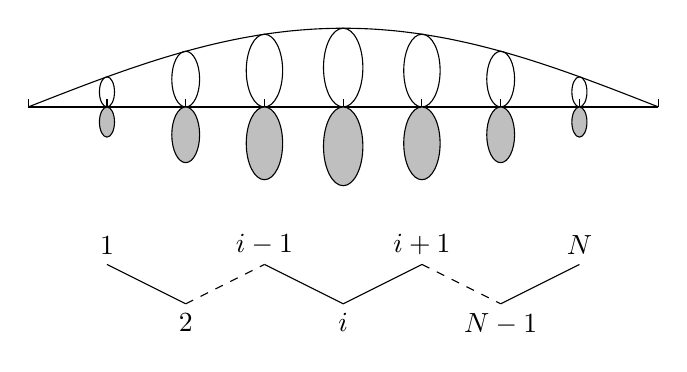
\begin{tikzpicture}
            \draw (0,0.5)node[above]{1}--(1,0)node[below]{2};
            \draw[dashed] (1,0)--(2,0.5);
            \draw (2,0.5)node[above]{\(i-1\)}--(3,0)node[below]{\(i\)}--(4,0.5)node[above]{\(i+1\)};
            \draw[dashed] (4,0.5)--(5,0);
            \draw (5,0)node[below]{\(N-1\)}--(6,0.5)node[above]{\(N\)};
            \draw (-1,2.5)--(7,2.5);
            \foreach \i in{-1,...,7}{
                \draw (\i,2.5)--(\i,2.6);
            }
            \draw[domain=0:1, smooth, variable=\x] plot ({8*\x -1}, {2.5+sin(\x * 3.14 r)});
            \foreach \i in {0,...,7}{
                \tikzmath{\x = sin(\i * 22.5);}
                \draw (\i-1,2.5+0.5*\x) ellipse (0.25*\x cm and 0.5*\x cm);
                \draw[fill=gray!50] (\i-1,2.5-0.5*\x) ellipse (0.25*\x cm and 0.5*\x cm);
            }
        \end{tikzpicture}
    \end{figure}

    \subsubsection*{Cyclic Polyenes}
    Consider a cyclic polyene of \(N\) atoms. By single-valuedness, we must have \(c_s^{(n)}=c_{s+N}^{(n)}\). It is analogous to a particle on a ring, and has orbital coefficients
    \begin{equation}\label{cyclic_polyene_coeff}
        c_s^{(n)}=\sqrt{\frac{1}{N}}\ee^{2\pi \ii ns/N}
    \end{equation}
    with energies
    \begin{equation}
        \epsilon_n=\alpha+2\beta\cos\frac{2\pi n}{N}\,.
    \end{equation}
    for \(-N/2< n\le N/2\).

    The energy levels can be conveniently viewed as the vertices of the \(N\)-gon inscribed in a circle with radius \(2\beta\) and centered at \(\alpha\). This is known as the \textit{Frost circle} construction.

    \begin{figure}
        \centering
        \begin{tikzpicture}
            \draw[->] (0,-2.3)--(0,2.3);
            \draw (0,-1.5)--(-0.1,-1.5)node[left]{\small\(\alpha+2\beta\)};
            \draw (0,0)--(-0.1,0)node[left]{\small\(\alpha\)};
            \draw (0,1.5)--(-0.1,1.5)node[left]{\small\(\alpha-2\beta\)};
            \draw (4.5,-1.5)--(5.5,-1.5);
            \draw (4.5,-0.514)--(5.5,-0.514);
            \draw (4.5,-0.414)--(5.5,-0.414);
            \draw (4.5,1.164)--(5.5,1.164);
            \draw (4.5,1.264)--(5.5,1.264);
            \begin{scope}[shift={(2.5,0)}]
                \foreach \i in {0,...,4}{
                    \draw (72*\i-90:1.5) circle (0.04);
                    \draw (72*\i-90:1.5) -- (72*\i-18:1.5);
                }
            \end{scope}
            \begin{scope}[shift={(8,0)}]
                \foreach \i in {0,...,5}{
                    \draw (60*\i-90:1.5) circle (0.04);
                    \draw (60*\i-90:1.5) -- (60*\i-30:1.5);
                }
            \end{scope}
            \draw (10,-1.5)--(11,-1.5);
            \draw (10,-0.7)--(11,-0.7);
            \draw (10,-0.8)--(11,-0.8);
            \draw (10,1.5)--(11,1.5);
            \draw (10,0.7)--(11,0.7);
            \draw (10,0.8)--(11,0.8);
        \end{tikzpicture}
        \caption{Frost circle construction for the energy levels of cyclic polyene.}
    \end{figure}

    This expression (\ref{cyclic_polyene_coeff}) of molecular orbitals is nice and compact, but the values are complex. We can make everything real by doing linear combinations of the degenerate orbitals and get
    \begin{align}
        \tilde{c}_s^{(0)}&=\sqrt{\frac{1}{N}}\\
        \tilde{c}_s^{(ns)}&=\sqrt{\frac{2}{N}}\sin\frac{2\pi ns}{N}\\
        \tilde{c}_s^{(nc)}&=\sqrt{\frac{2}{N}}\cos\frac{2\pi ns}{N}\\
        \tilde{c}_s^{(\frac{N}{2})}&=\sqrt{\frac{1}{N}}(-1)^s\,,
    \end{align}
    where the \(N/2\) orbital exists only if \(N\) is even.

    \subsection{Is H\"{u}ckel Theory Predictive?}
    \subsubsection{Total Energies}
    By H\"{u}ckel theory, we have worked out a set of molecular orbitals for a bunch of electrons. The next question is, how to put these electrons into the orbitals, and how to work out the total energy of the system?

    By Pauli's principle, we can only put two electrons with opposite spins in the same orbital. And a system always wants to keep its energy as low as possible. Therefore, we occupy the orbitals from the lowest to the highest until we have put in all of the electrons. To work out the total energy, we simply need to add up all the orbital energies that each electron sits in.\footnote{The answer is actually not that simple... See later.} We define an \textit{occupation number}, \(f_n\), as the number of electrons in orbital \(n\) (it would be 0, 1 or 2), then since we assumed all electrons are independent under our effective potential approximation,
    \begin{equation}
        E_{\text{H\"{u}ckel}}=\sum_n f_n\epsilon_n\,.
    \end{equation}

    \subsubsection{Delocalisation Energy}
    One of the triumphs of H\"{u}ckel theory was to rationalise the stability of benzene and other aromatics, showing that they are made more stable by a significant delocalisation energy.

    Let's take benzene as an example. The molecular orbital diagrams of benzene and a normal double bond (ethene) are shown in the figure.
    \begin{figure}[ht!]
        \centering
        \begin{tikzpicture}
            \draw (0,-0.7)--(0.8,-0.7);
            \draw (0,0.7)--(0.8,0.7);
            \draw (1.2,-1.4)--(2,-1.4);
            \draw (1.2,1.4)--(2,1.4);
            \draw (2.4,-0.7)--(3.2,-0.7);
            \draw (2.4,0.7)--(3.2,0.7);
            \draw[thick,->] (1.55,-1.7)--(1.55,-1.1);
            \draw[thick,<-] (1.65,-1.7)--(1.65,-1.1);
            \draw[thick,->] (0.35,-1)--(0.35,-0.4);
            \draw[thick,<-] (0.45,-1)--(0.45,-0.4);
            \draw[thick,->] (2.75,-1)--(2.75,-0.4);
            \draw[thick,<-] (2.85,-1)--(2.85,-0.4);
            \node at (1.6,2.5) {Benzene};
            \node at (3.3,-1.4)[right]{\small\(\alpha+2\beta\)};
            \node at (3.3,-0.7)[right]{\small\(\alpha+\beta\)};
            \node at (3.3,1.4)[right]{\small\(\alpha-2\beta\)};
            \node at (3.3,0.7)[right]{\small\(\alpha-\beta\)};

            \draw (7,-0.7)--(7.8,-0.7);
            \draw (7,0.7)--(7.8,0.7);
            \draw[thick,->] (7.35,-1)--(7.35,-0.4);
            \draw[thick,<-] (7.45,-1)--(7.45,-0.4);
            \node at (7.9,-0.7)[right]{\small\(\alpha+\beta\)};
            \node at (7.9,0.7)[right]{\small\(\alpha-\beta\)};
            \node at (7.4,2.5) {Ethene};
        \end{tikzpicture}
    \end{figure}

    The delocalisation energy is the energy difference between the total energy of the delocalised molecule and the energy if the \(\pi\) system were localised i.e. each \(\pi\) bond is treated separately. For benzene, this is
    \begin{align}
        E_{\text{deloc}}&=[2(\alpha+2\beta)+4(\alpha+\beta)]-[6(\alpha+\beta)]\notag\\
        &=2\beta\,.
    \end{align}
    We see that H\"{u}ckel theory predicts the extra stability of benzene through delocalisation i.e. \textit{aromaticity}.

    We can calculate the delocalisation energy for more aromatic compounds. The results are shown in the table below.
    \renewcommand{\arraystretch}{1.2}
    \begin{table}[ht!]
        \centering
        \begin{tabular}{lccc}
            \toprule
            Molecule & Theory & Experiment / \(\!\unit{kJ}\unit{mol}^{-1}\) & Estimated \(\abs{\beta}\) / \(\!\unit{kJ}\unit{mol}^{-1}\) \\ \midrule
            benzene & \(2\beta\) & -155 & 77.7 \\
            naphthalene & \(3.68\beta\) & -315 & 85.7 \\
            anthracene & \(5.32\beta\) & -441 & 82.7 \\
            phenanthrene & \(5.45\beta\) & -462 & 84.8 \\ \bottomrule
        \end{tabular}
    \end{table}

    Two conclusions can be drawn from this. First, the close parallel between the H\"{u}ckel theory prediction on the variation of the delocalisation energy for the series, as compared to experiment, which indicates that even such crude calculations are able to reproduce a significant trend. Taking \(\beta\) to be about \(-80\unit{kJ}\unit{mol}^{-1}\) leads to a reasonable agreement between predicted and experimental delocalisation energies. Second, phenanthrene (three benzene rings fused in a ``zig-zag'' fashion) is slightly more stable than anthracene (three benzene rings fused in a straight line). This trend continues for larger systems: the annulation to give “zig-zag” forms are indeed experimentally more stable than the corresponding linear ones.

    It is impressive that our very crude theory is able to give some interesting, semi-quantitative, results.

    \subsubsection{Orbital Energies}
    Matters look less rosy if we consider a different type of measurement of \(\beta\), using ionisation energies.

    Recall that the first ionisation energy is the minimum energy required to remove an electron from a molecule, and therefore it is reasonable to suppose that the electron removed comes from HOMO. Since, according to H\"{u}ckel theory, the energy of an orbital can be written in the form
    \begin{equation}
        \epsilon=\alpha+x\beta\,,
    \end{equation}
    where \(x\) is a suitable coefficient which depends on the molecule, one may suppose that if we take a series of molecules (e.g. benzene, naphthalene, anthracene, \textit{etc.}), for which the \(x\) can be calculated, and plot the ionisation energy as a function of \(x\), then the slope of such a (hopefully linear) curve would yield \(\beta\), whereas the intercept would yield \(\alpha\). It turns out that a least-squares fit yields
    \begin{equation}
        \text{Experimental Orbital Energy}=-685+(-239\pm 16)x\unit{kJ}\unit{mol}^{-1}\,.
    \end{equation}
    We obtained a value of \(\beta\approx -240\unit{kJ}\unit{mol}^{-1}\) --- almost three times as large as what we've predicted using total energy!

    In fact this turns out to be a quite general feature of H\"{u}ckel theory. Experiments which depend on the energy of single orbitals turn out to yield values of \(\beta\) which are always roughly a factor of two larger than those based on total energies, in which the energies of many orbitals are summed together.

    The explanation for this behaviour can be found by considering the manner in which electron-electron interactions are dealt with in the Hamiltonian \(\hat{H}\). Recall that the \(\hat{H}\) is an effective Hamiltonian in which an electron sees the average field due to all other electrons. In other words, electron 1 sees a field due to the average of electrons 2, 3, \textit{etc.}, and this field, in addition to the field due to the nuclear framework, determines the energy eigenvalue of electron 1. Similarly, electron 2 sees the average field of electron 1, electron 3, \textit{etc.}, and its energy eigenvalue reflects these interactions as well.

    Therefore, if we add the energy eigenvalue of electron 1 and electron 2, we have counted twice the average electrostatic interaction between electron 1 and electron 2. This is exactly what is done in our method of calculating the total \(\pi\)-energy: we simply add the energy of all occupied levels. On the other hand, if we are dealing with purely the energy of a single energy level, there is no double counting. Therefore, it should not be surprising that methods used to estimate \(\beta\) based on the total energies yield values about \(1/2\) of that from ionisation potential experiments.\footnote{To fix such a problem, one uses theories that treat the effective Hamiltonian more carefully. See Hartree--Fock theory.}
    
    \begin{ex}
        We will illustrate our idea with a toy model. Consider a 3-electron system with only repulsion.
        \begin{figure}[ht!]
            \centering
            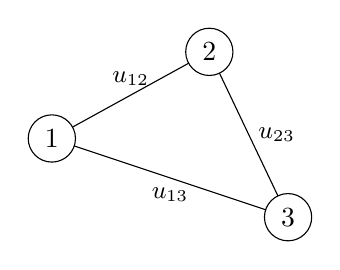
\begin{tikzpicture}
                \draw (0,0)--node[above]{\small\(u_{12}\)}(2,1.1);
                \draw (3,-1)--node[right]{\small\(u_{23}\)}(2,1.1);
                \draw (3,-1)--node[below]{\small\(u_{13}\)}(0,0);
                \draw[fill=white] (0,0) circle (0.3);
                \node at (0,0) {1};
                \draw[fill=white] (2,1.1) circle (0.3);
                \node at (2,1.1) {2};
                \draw[fill=white] (3,-1) circle (0.3);
                \node at (3,-1) {3};
            \end{tikzpicture}
        \end{figure}

        The energy of each electron is
        \begin{equation}
            \begin{aligned}
                \epsilon_1&=u_{12}+u_{13}\\
                \epsilon_2&=u_{12}+u_{23}\\
                \epsilon_3&=u_{13}+u_{23}\,.
            \end{aligned}
        \end{equation}
        If we directly sum up the individual energy of each electron, we get
        \begin{equation}
            E=\epsilon_1+\epsilon_2+\epsilon_3=2u_{12}+2u_{13}+2u_{23}\,.
        \end{equation}
        However, the actual total energy should be
        \begin{equation}
            E_{\text{total}}=u_{12}+u_{13}+u_{23}\,.
        \end{equation}
        We have double-counted all the interactions!
    \end{ex}

    \subsection{Populations and Bond Orders}
    While the MOs produce a delocalised picture of bonding in a molecule, it is often helpful to be able to ask more specific questions, such as whether the electrons are concentrated on particular atoms, or to probe the relative strengths of bonding between two neighbouring atoms. With this information, we would, for example, be able to say whether in butadiene the canonical picture of two terminal double bonds is the most appropriate.

    For some state \(\ket{\phi}\), define the \textit{projection operator}
    \begin{equation}
        \hat{q}=\ket{\phi}\bra{\phi}\,.
    \end{equation}
    What is the meaning of this? Let's act it on some general state \(\ket{\psi}\). We get
    \begin{equation}
        \hat{q}\ket{\psi}=\ket{\phi}\braket{\phi}{\psi}\,.
    \end{equation}
    It returns the state \(\ket{\phi}\) we are projecting onto, scaled by the inner product of two states \(\braket{\phi}{\psi}\). As its name tells, it ``projects'' the state \(\ket{\psi}\) on to \(\ket{\phi}\).

    Let's see how it acts on the molecular orbitals. Let's evaluate the expectation value of a molecular orbital under the projection operator of an atomic orbital \(\hat{q}_i=\ket{\phi_i}\bra{\phi_i}\). Since under H\"{u}ckel's approximation, the atomic orbitals \(\{\phi_s\}\) are orthonormal, we have
    \begin{align}
        \expval{\hat{q}_i}{\psi_n}&=\braket{\sum_s c_s^{(n)}\phi_s}{\phi_i}\braket{\phi_i}{\sum_t c_t^{(n)}\phi_t}\notag\\
        &=\left(\sum_s c_s^{(n)*}\delta_{is}\right)\left(\sum_t c_t^{(n)}\delta_{it}\right)\notag\\
        &=c_i^{(n)*}c_i^{(n)}=\abs{c_i^{(n)}}^2\,.
    \end{align}
    The effect is to extract the squared modulus of the coefficient of the given atomic orbital, which can in turn be thought of as the population on that atom from the orbital.

    We may therefore work out the total population on atom \(s\), by summing together such quantities
    \begin{align}
        q_s&=\sum_n f_n\expval{\hat{q}_s}{\psi_n}\notag\\
        &=\sum_n f_n\abs{c_s^{(n)}}^2\,,
    \end{align}
    where recall \(f_n\) is the occupation number of orbital \(n\).

    Analogously, we may define the operator
    \begin{equation}
        \hat{p}_{st}=\frac{1}{2}\left(\ket{\phi_s}\bra{\phi_t}+\ket{\phi_t}\bra{\phi_s}\right)\,,
    \end{equation}
    which combines the sign and amplitude information of the orbital coefficients from neighbouring sites, giving a measure of the bonding. The \(\ket{\phi_s}\bra{\phi_t}\) and its Hermitian conjugate \(\ket{\phi_t}\bra{\phi_s}\) are averaged to make this operator Hermitian. Summing over orbitals, the bond order between two neighbouring atoms \(s\) and \(t\) can be calculated by
    \begin{align}
        p_{st}&=\sum_{n}f_n\expval{\hat{p}_{st}}{\psi_n}\notag\\
        &=\sum_n f_n \Re[{c_s^{(n)}}^*c_t^{(n)}]\,.
    \end{align}
    The sign and magnitude of \(p_{st}\) indicate the bonding, with \(+1\) indicating one bonding contribution, and \(-1\) one anti-bonding contribution.

    \subsection{Alternant Hydrocarbons}
    A useful application of H\"{u}ckel theory is to rationalise the differing properties of \textit{alternant} and \textit{non-alternant} hydrocarbons. An alternant hydrocarbon is one in which the carbon atoms can be divided into a ``starred'' class and a ``non-starred'' class, such that each starred atom is neighboured by only unstarred atoms, and vice versa. The starred class is generally taken to be the larger of the two classes of atoms. Two examples in \cref{Fig:Alternant_Hydrocarbon} illustrate this.
    \begin{figure}
        \centering
        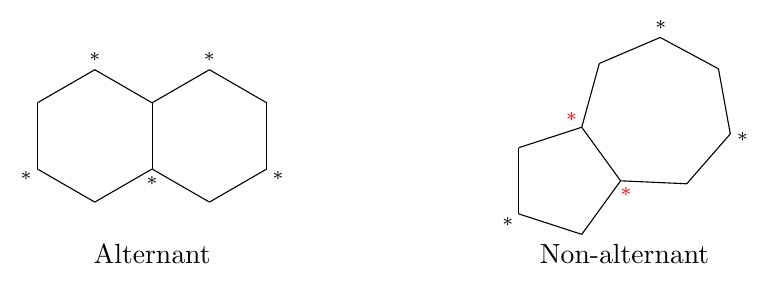
\begin{tikzpicture}
            \node at (0,0){
                \scriptsize\chemfig{*6(\charge{210:3pt=\(*\)}{}--\charge{270:3pt=\(*\)}{}*6(--\charge{330:3pt=\(*\)}{}--\charge{90:3pt=\(*\)}{}-)--\charge{90:3pt=\(*\)}{}--)}
            };
            \node at (0,-1.5){Alternant};
            \node at (6,0){
                \scriptsize\chemfig{*5(\charge{216:3pt=\(*\)}{}--\charge{295.7:3pt=\color{red}\(*\)}{}*7(--\charge{344.5:3pt=\(*\)}{}--\charge{87.3:3pt=\(*\)}{}--)-\charge{136.3:3pt=\color{red}\(*\)}{}--)}
            };
            \node at (6,-1.5){Non-alternant};
        \end{tikzpicture}
        \caption{Examples of alternant and non-alternant hydrocarbons.}
        \label{Fig:Alternant_Hydrocarbon}
    \end{figure}

    In H\"{u}ckel theory, alternant hydrocarbons have the following properties:
    \begin{enumerate}[topsep=0pt,label=(\roman*)]
        \item The energy levels of alternant hydrocarbons are symmetrically paired around an \(\alpha\), such that if orbital \(n\) has energy \(\epsilon_n=\alpha+k\beta\) then its pair, orbital \(N-n+1\) has energy \(\epsilon_{N-n+1}=\alpha-k\beta\).
        \item The AO coefficients in any pair of complementary orbitals are related by changing the sign of the coefficients on the unstarred atoms.
        \item In a neutral alternant, the atomic populations in the ground state are precisely unity.
        \item In odd-alternants, there is a non-bonding orbital, with nonzero coefficients only on the starred atoms, and the sum of coefficients on starred atoms which surround an unstarred site is zero.
    \end{enumerate}

    \subsection{Heteroconjugated Systems and Perturbation Theory}
    Suppose we want to use H\"{u}ckel theory to solve a heteroconjugated system (a conjugated system involving more than one type of atoms) e.g. pyridine or pyrrole. Since nitrogen has a different energy than carbon, and a C-C \(\pi\) bond would have a different strength than a C-N \(\pi\) bond, we should set a different \(\alpha\) and \(\beta\) value for them.

    \subsubsection{Non-degenerate Perturbation Theory}
    \begin{figure}
        \centering
        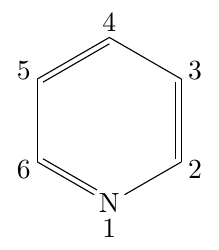
\begin{tikzpicture}
            \node at (0,0){\chemfig{*6(\charge{210:4pt=6}{}=\charge{270:4pt=1}{N}-\charge{330:4pt=2}{}=\charge{30:4pt=3}{}-\charge{90:4pt=4}{}=\charge{150:4pt=5}{}-)}};
        \end{tikzpicture}
        \caption{Numbering of pyridine.}
    \end{figure}

    Suppose we want to solve for pyridine. We use the numbering shown in the figure. Then the \(\pi\) system has the Hamiltonian matrix
    \begin{equation}
        \mathsf{H}=\begin{pmatrix}
            \alpha_{\mathrm{N}} & \beta_{\mathrm{NC}} & 0 & 0 & 0 & \beta_{\mathrm{NC}} \\
            \beta_{\mathrm{NC}} & \alpha & \beta & 0 & 0 & 0 \\
            0 & \beta & \alpha & \beta & 0 & 0 \\
            0 & 0 & \beta & \alpha & \beta & 0 \\
            0 & 0 & 0 & \beta & \alpha & \beta \\
            \beta_{\mathrm{NC}} & 0 & 0 & 0 & \beta & \alpha
        \end{pmatrix}\,.
    \end{equation}
    Let's set \(\alpha_{\mathrm{N}}=\alpha+0.5\beta\) and \(\beta_{\mathrm{NC}}=0.8\beta\).

    Of course we can solve this Hamiltonian matrix directly, but isn't this system (and the Hamiltonian of course) too similar to benzene, which we already know the solution? It might be helpful to think of this Hamiltonian as the Hamiltonian for benzene, plus a small modification, which we call a \textit{perturbation}
    \begin{align}
        \mathsf{H}&=\mathsf{H}_0+\mathsf{\Delta H}\notag\\
        &=\begin{pmatrix}
            \alpha & \beta & 0 & 0 & 0 & \beta \\
            \beta & \alpha & \beta & 0 & 0 & 0 \\
            0 & \beta & \alpha & \beta & 0 & 0 \\
            0 & 0 & \beta & \alpha & \beta & 0 \\
            0 & 0 & 0 & \beta & \alpha & \beta \\
            \beta & 0 & 0 & 0 & \beta & \alpha
        \end{pmatrix} + \begin{pmatrix}
            0.5 \beta & -0.2\beta & 0 & 0 & 0 & -0.2\beta \\
            -0.2\beta & 0 & 0 & 0 & 0 & 0 \\
            0 & 0 & 0 & 0 & 0 & 0 \\
            0 & 0 & 0 & 0 & 0 & 0 \\
            0 & 0 & 0 & 0 & 0 & 0 \\
            -0.2\beta & 0 & 0 & 0 & 0 & 0 \\
        \end{pmatrix}\,,
    \end{align}
    where \(H_0\) is the Hamiltonian of our reference system, benzene in this case, and \(\Delta H\) is our perturbation. We hope that, by modifying the Hamiltonian only slightly, the molecular orbitals only change slightly as well. Then, it might be possible to express, even if only approximately, the energy levels and MOs of the perturbed Hamiltonian (e.g. pyridine) in terms of the unperturbed one (e.g. benzene).

    This is the topic of \textit{perturbation theory}. It will be covered in great depth in course \textit{C7: Further Quantum Mechanics} (and in even greater depth in Mathematical Tripos Part II \textit{Principles of Quantum Mechanics}). We will show some simple results here.

    \begin{figure}
        \centering
        \begin{tikzpicture}
            \node at (0,5) {\chemfig{[,0.7]*6(=-=-=-)}};
            \draw (-0.4,3)--(0.4,3);
            \draw (-1.5,2)--(-0.7,2);
            \draw (1.5,2)--(0.7,2);
            \draw (-1.5,0)--(-0.7,0);
            \draw (1.5,0)--(0.7,0);
            \draw (-0.4,-1)--(0.4,-1);
            \node at (4,5) {\chemfig{[,0.7]*6(={N}-=-=-)}};
            \draw (3.5,2.7)--(4.5,2.7);
            \draw (3.5,2.1)--(4.5,2.1);
            \draw (3.5,1.7)--(4.5,1.7);
            \draw (3.5,0)--(4.5,0);
            \draw (3.5,-0.16)--(4.5,-0.16);
            \draw (3.5,-0.76)--(4.5,-0.76);
            \draw[dashed,->] (0.5,-1)--(3.4,-0.76);

            \draw[->] (6.5,0)--(10.5,0)node[below]{\small\(\norm{\Delta H}\)};
            \draw[->] (6.5,0)--(6.5,4)node[left]{\(\epsilon\)};
            \draw[fill=black] (7,0.5) circle (0.03);
            \draw[domain=0:3, smooth, variable=\x,thick] plot ({\x+7}, {0.5+0.8*\x-0.05*\x*\x});
            \draw[domain=0:3, smooth, variable=\x,dashed] plot ({\x+7}, {0.5+0.8*\x});
            \draw[dashed] (7,0.5)--(11,0.5);
            \draw[dashed] (10,2.45)--(10.5,2.45);
            \draw[dashed] (10,2.9)--(11,2.9);
            \draw[->] (10.1,0.5)--node[right]{\small\(\Delta\epsilon_i\)}(10.1,2.45);
            \draw[->] (10.8,0.5)--node[right]{\small\(\Delta^{(1)}\epsilon_i\)}(10.8,2.9);
            \draw (7,0.1)--(7,0)node[below]{\(0\)};
            \draw (6.6,0.5)--(6.5,0.5)node[left]{\(\epsilon_i\)};
        \end{tikzpicture}
        \caption{We expect that, by changing the Hamiltonian slightly, the molecular orbital energies will also shift only slightly. This shift should be smoothly dependent on the ``size'' of the perturbation. We can easily work out this change in first order.}
    \end{figure}

    We will first work on the case where the molecular orbital energy levels are non-degenerate.

    \begin{prop}
        Let \(\hat{H}\) be a perturbed Hamiltonian that can be written as
        \begin{equation}
            \hat{H}=\hat{H}_0+\Delta \hat{H}\,.
        \end{equation}
        Suppose we know that the unperturbed Hamiltonian \(\hat{H}_0\) has a normalised non-degenerate eigenstate \(\ket{\psi_i}\) and corresponding eigenvalue \(\epsilon_i\). Then, after the perturbation, the corresponding eigenvalue is changed by
        \begin{equation}
            \Delta^{(1)}\epsilon_i=\expval{\Delta \hat{H}}{\psi_i}
        \end{equation}
        to first order.
    \end{prop}
    \begin{proof}
        We will show this result loosely. For a rigorous proof, see C7 or Principles of Quantum Mechanics.

        Suppose when we change \(\hat{H}_0\) to \(\hat{H}_0+\Delta \hat{H}\), \(\psi_i\) has changed to \(\psi_i+\Delta\psi_i\), then the energy has changed to
        \begin{equation}
            \epsilon_i+\Delta\epsilon_i=\frac{\expval{\hat{H}_0+\Delta \hat{H}}{\psi_i+\Delta\psi_i}}{\braket{\psi_i+\Delta\psi_i}{\psi_i+\Delta\psi_i}}\,.
        \end{equation}
        Note that to change \(\psi_i\) meaningfully, \(\Delta\psi_i\) must be orthogonal to \(\psi_i\) since scaling not does actually change the state, so \(\braket{\Delta\psi_i}{\psi_i}=0\). Expand to the first order in \(\Delta\), we get
        \begin{align}
            \epsilon_i+\Delta^{(1)}\epsilon_i&=\frac{\expval{\hat{H}_0}{\psi_i}+\mel{\Delta\psi_i}{\hat{H}_0}{\psi_i}+\mel{\psi_i}{\Delta \hat{H}}{\psi_i}+\mel{\psi_i}{\hat{H}_0}{\Delta\psi_i}}{\braket{\psi_i}{\psi_i}+\braket{\psi_i}{\Delta\psi_i}+\braket{\Delta\psi_i}{\psi_i}}\notag\\
            &=\epsilon_i+\mel{\Delta\psi_i}{\hat{H}_0}{\psi_i}+\mel{\psi_i}{\Delta \hat{H}}{\psi_i}+\mel{\psi_i}{\hat{H}_0}{\Delta\psi_i}\,.
        \end{align}
        Since \(H_0\psi_i=\epsilon_i\psi_i\), we have
        \begin{equation}
            \mel{\psi_i}{\hat{H}_0}{\Delta\psi_i}^*=\mel{\Delta\psi_i}{\hat{H}_0}{\psi_i}=\epsilon_i\braket{\Delta\psi_i}{\psi_i}=0\,.
        \end{equation}
        Hence,
        \begin{equation}
            \Delta^{(1)}\epsilon_i=\expval{\Delta \hat{H}}{\psi_i}
        \end{equation}
        as claimed.\qed
    \end{proof}

    \subsection{Degenerate Perturbation Theory}
    When applying this to degenerate orbitals you must take a little more care to recover a well-defined solution. Recall that in the reference system, any orthogonal linear combination of two degenerate orbitals would still have the same energy and can be regarded as equally valid. Once the perturbation has been applied however, the different linear combinations may produce different energy changes. In such cases, the perturbation is said to break the degeneracy. To recover a well-defined energy change, we resort to the variational principle again, asking: which combination of the degenerate states produces the lowest energy under the perturbation? This is none other than our old friend the secular problem, and we must therefore diagonalize a small matrix consisting of just the degenerate states to solve it.

    If there are some degenerate eigenstates of \(\hat{H}_0\), denoted \(\psi_i\), then we may write out the perturbation \(\Delta \hat{H}\) in the basis of these two orbitals
    \begin{equation}
        \Delta H_{ij}=\mel{\psi_i}{\Delta \hat{H}}{\psi_j}\,.
    \end{equation}
    To determine the appropriate energies, we then solve
    \begin{equation}
        (\mathsf{\Delta H}-\Delta\epsilon\mathsf{I})\vb{c}=\vb{0}\,.
    \end{equation}
    The eigenvalues, \(\Delta\epsilon\) are the appropriate perturbed energies, and the eigenvectors give the appropriate linear combination of \(\psi_i\) which has that perturbed energy.
    \begin{ex}
        Let's try this on the occupied orbitals of pyridine. We use the numbering as before, thinking it as a perturbation on the reference system benzene, whose orbital coefficients and energies are well-known
        \begin{align}
            \vb{c}^{(0)}&=\frac{1}{\sqrt{6}}\begin{pmatrix}
                1 & 1 & 1 & 1 & 1 & 1
            \end{pmatrix}\tp & E^{(0)}&=\alpha+2\beta \\
            \vb{c}^{(1c)}&=\frac{1}{\sqrt{12}}\begin{pmatrix}
                2 & 1 & -1 & -2 & -1 & 1
            \end{pmatrix}\tp & E^{(1c)}&=\alpha+\beta \\
            \vb{c}^{(1s)}&=\frac{1}{2}\begin{pmatrix}
                0 & 1 & 1 & 0 & -1 & -1
            \end{pmatrix}\tp & E^{(1s)}&=\alpha+\beta\,.
        \end{align}
        The perturbation is
        \begin{equation}
            \mathsf{\Delta H}=\frac{\beta}{10}\begin{pmatrix}
                5 & -2 & 0 & 0 & 0 & -2 \\
                -2 & 0 & 0 & 0 & 0 & 0 \\
                0 & 0 & 0 & 0 & 0 & 0 \\
                0 & 0 & 0 & 0 & 0 & 0 \\
                0 & 0 & 0 & 0 & 0 & 0 \\
                -2 & 0 & 0 & 0 & 0 & 0 \\
            \end{pmatrix}\,.
        \end{equation}

        The state \(\ket{\psi_0}\) is non-degenerate, so
        \begin{align}
            \Delta^{(1)}\epsilon_0&=\expval{\Delta\hat{H}}{\psi_0}\notag\\
            &=\vb{c}^{(0)\dagger}\mathsf{\Delta H}\vb{c}^{(0)}\notag\\
            &=-\frac{\beta}{20}\,.
        \end{align}

        The next two orbitals are degenerate, so we need to use degenerate perturbation theory. We evaluate
        \begin{align}
            \expval{\Delta\hat{H}}{\psi_{1c}}&=\frac{\beta}{30}\\
            \expval{\Delta\hat{H}}{\psi_{1s}}&=0\\
            \mel{\psi_{1c}}{\Delta\hat{H}}{\psi_{1s}}&=0\,,
        \end{align}
        so the matrix
        \begin{equation}
            \mathsf{\Delta H}=\begin{pmatrix}
                +\frac{\beta}{30} & 0 \\
                0 & 0
            \end{pmatrix}
        \end{equation}
        is already diagonalised. The variations in energies are
        \begin{equation}
            \Delta^{(1)}\epsilon=+\frac{\beta}{30},0\,.
        \end{equation}

        It turns out that the matrix \(\mathsf{\Delta \hat{H}}\) is automatically diagonalised for us because we have chosen a good basis. If we instead rotate the unperturbed orbitals to
        \begin{align}
            {\vb{c}^{(1c)}}'&=\frac{1}{\sqrt{12}}\begin{pmatrix}
                1 & -1 & -2 & -1 & 1 & 2
            \end{pmatrix}\tp\\
            {\vb{c}^{(1s)}}'&=\frac{1}{2}\begin{pmatrix}
                1 & 1 & 0 & -1 & -1 & 0
            \end{pmatrix}\tp
        \end{align}
        using the same perturbation matrix, then we would get
        \begin{align}
            \expval{\Delta\hat{H}}{\psi_{1c}'}&=\frac{\beta}{120}\\
            \expval{\Delta\hat{H}}{\psi_{1s}'}&=\frac{\beta}{40}\\
            \mel{\psi_{1c}'}{\Delta\hat{H}}{\psi_{1s}'}&=\frac{\beta}{20\sqrt{12}}\,,
        \end{align}
        giving
        \begin{equation}
            \mathsf{\Delta H}'=\begin{pmatrix}
                \frac{\beta}{120} & \frac{\beta}{20\sqrt{12}} \\
                \frac{\beta}{20\sqrt{12}} & \frac{\beta}{40}
            \end{pmatrix}\,.
        \end{equation}
        Diagonalising these will still give us the correct eigenvalues \(\Delta^{(1)}\epsilon=+\frac{\beta}{30},0\).

        A lesson is to put nodes on special atoms.
    \end{ex}

    \section{Many-electron Wavefunction}
    Throughout the last chapter, we assumed the wavefunction to take the form of a \textit{Hartree product}
    \begin{equation}\label{orbital_assumption}
        \Psi(\vb{r}_1,\dots,\vb{r}_n)=\psi_1(\vb{r}_1)\dots\psi_n(\vb{r}_n)\,.
    \end{equation}
    This makes the problem simple and easy to solve, but it has a severe problem --- a Hartree product does not obey Pauli principle. To take a step further, we must consider spins.

    \subsection{Spin}
    Recall that electron has spin \(s=\frac{1}{2}\), so it has two possible spin states \(s_z=+\frac{1}{2},-\frac{1}{2}\). The two \(s_z=+\frac{1}{2},-\frac{1}{2}\) spin eigenfunctions are represented by \(\alpha(\omega)\) and \(\beta(\omega)\) respectively, where \(\omega\) is a fictitious coordinate to keep track of which electron a spin belongs to (and is a simplification of some quantum field theory formulation). We have the spin magnitude squared operator \(\hat{s}^2(\omega)\), and the operator for the \(z\) component of spin \(\hat{s}_z(\omega)\), which acts on the spin eigenstate \(\sigma(\omega)\) by
    \begin{align}
        \hat{s}^2\sigma(\omega)&=\hbar^2s(s+1)\sigma(\omega)\\
        \hat{s}_z\sigma(\omega)&=\hbar s_z\sigma(\omega)\,.
    \end{align}

    A many-electron wavefunction also has spin, and corresponding spin operators. The total \(z\) component of spin operator takes the simple form
    \begin{equation}
        \hat{S}_z(\omega_1,\omega_2,\dots,\omega_n)=\sum_{i=1}^{n}\hat{s}_z(\omega_i)
    \end{equation}
    because the component of a vector is a scalar and we can add them simply. There is a corresponding total spin square magnitude operator, \(\hat{S}^2\), but its form is not a simple sum and not trivial to apply, and will not be needed in this course.\footnote{The most convenient form is written in terms of ladder operators, as
    \begin{equation}
        \hat{S}^2=\hat{S}_+\hat{S}_-+(\hat{S}_z)^2-\hbar\hat{S}_z\,.
    \end{equation}}
    For a total spin eigenfunction \(\Sigma(\omega_1,\dots,\omega_n)\), the eigenvalue equations are
    \begin{align}
        \hat{S}_z\Sigma&=\hbar M_S\Sigma\\
        \hat{S}^2\Sigma&=\hbar^2 S(S+1)\Sigma\,,
    \end{align}
    where for a given \(S\), \(M_S=-S,-S+1,\dots,S-1,S\).

    When writing a complete wavefunction, we must also consider the spin part of the wavefunction in addition to the spatial part. Therefore, a complete wavefunction should be
    \begin{equation}
        \Psi(\vb{r}_1,\dots,\vb{r}_n;\omega_1,\dots,\omega_n)\,.
    \end{equation}

    The most important feature for electrons is that they are fermions. An important rule for fermions is that the wavefunction must be antisymmetric with respect to exchange of electrons, so that
    \begin{equation}
        \Psi(\dots,\vb{r}_i,\dots,\vb{r}_j,\dots,\omega_i,\dots,\omega_j,\dots)=-\Psi(\dots,\vb{r}_j,\dots,\vb{r}_i,\dots,\omega_j,\dots,\omega_i,\dots)\,.
    \end{equation}
    Notice that by exchanging the electrons, we exchange both the spatial coordinates and the spin coordinates.
    
    As one can easily see, a simple Hartree product does not obey this condition --- we need to find some ways to construct antisymmetric total wavefunction from one-electron wavefunctions (orbitals). As you have seen in IB, one strategy of constructing an antisymmetric wavefunction is to construct symmetric and antisymmetric spatial and spin wavefunctions separately, then combine the symmetric spatial wavefunction with the antisymmetric spin wavefunction and vice versa. For two electrons with different spatial wavefunctions, the possible wavefunctions are
    \begin{align}
        \Psi_{\text{triplet}}&=\frac{1}{\sqrt{2}}[\psi_1(\vb{r}_1)\psi_2(\vb{r}_2)-\psi_2(\vb{r}_1)\psi_1(\vb{r}_2)]\times\begin{cases}
            \alpha(\omega_1)\alpha(\omega_2)\\
            \frac{1}{\sqrt{2}}[\alpha(\omega_1)\beta(\omega_2)+\beta(\omega_1)\alpha(\omega_2)]\\
            \beta(\omega_1)\beta(\omega_2)
        \end{cases}\\
        \Psi_{\text{singlet}}&=\frac{1}{\sqrt{2}}[\psi_1(\vb{r}_1)\psi_2(\vb{r}_2)+\psi_2(\vb{r}_1)\psi_1(\vb{r}_2)]\times\frac{1}{\sqrt{2}}[\alpha(\omega_1)\beta(\omega_2)-\beta(\omega_1)\alpha(\omega_2)]\,.
    \end{align}
    The triplet state has \(S=1\) and \(M_S=-1,0,1\). The singlet state has \(S=0\) and \(M_S=0\).

    \subsection{Slater Determinants}
    The above method worked well for systems with two electrons, but it becomes increasingly painful for more and more electrons. We hope to find a more general and convenient method of constructing antisymmetric wavefunctions. It turns out that in mathematics, there is an object that is always antisymmetric --- that is a determinant.

    Because the electron exchanges in Pauli principle affect both the spatial and spin coordinates of an electron, it is convenient to group them together as a single coordinate \(\vb{x}=(\vb{r},\omega)\). We can also combine the spatial and spin orbitals together to form a \textit{spin-orbital}
    \begin{equation}
        \chi(\vb{x})\equiv\psi^{\sigma}(\vb{x})=\psi(\vb{r})\sigma(\omega)\,.
    \end{equation}

    By the property that a determinant changes the sign when we exchange any two columns or rows, we are guaranteed that
    \begin{equation}
        \Psi=\frac{1}{\sqrt{2}}\begin{pmatrix}
            \chi_a(\vb{x}_1) & \chi_b(\vb{x}_1) \\
            \chi_a(\vb{x}_2) & \chi_b(\vb{x}_2) \\
        \end{pmatrix}=\frac{1}{\sqrt{2}}[\chi_a(\vb{x}_1)\chi_b(\vb{x}_2)-\chi_b(\vb{x}_1)\chi_a(\vb{x}_2)]
    \end{equation}
    is antisymmetric with respect to the exchange of coordinates \(\vb{x}_1\) and \(\vb{x}_2\), since exchanging the coordinates is equivalent to exchanging the two rows. Additionally, if the spin-orbitals are normalised, this determinant is also normalised. This can be easily generalised. For \(n\) spin-orbitals, a \textit{Slater determinant} is defined as
    \begin{equation}
        \Psi=\frac{1}{\sqrt{n!}}\begin{vmatrix}
            \chi_a(\vb{x}_1) & \chi_b(\vb{x}_1) & \cdots & \chi_r(\vb{x}_1) \\
            \chi_a(\vb{x}_2) & \chi_b(\vb{x}_2) & \cdots & \chi_r(\vb{x}_2) \\
            \vdots & \vdots & \ddots & \vdots \\
            \chi_a(\vb{x}_n) & \chi_b(\vb{x}_n) & \cdots & \chi_r(\vb{x}_n)
        \end{vmatrix}\,.
    \end{equation}
    This is guaranteed to be antisymmetric, and since a \(n\times n\) determinant can be expanded into \(n!\) terms, it is normalised given that the spin orbitals are orthonormal. Sometimes, we denote it by the shorthand
    \begin{equation}
        \Psi=\frac{1}{\sqrt{n!}}\abs{\chi_a\chi_b\dots\chi_r}\,.
    \end{equation}

    \subsubsection{Two-Electron System}
    Finally we are going to solve the Schr\"{o}dinger equation, starting from a simple two-electron system. Let's observe the form of the electronic Hamiltonian (in atomic units)\footnote{Again, you can either include \(V^{\text{n-n}}\) to the electronic Hamiltonian or not --- it doesn't matter. It's just a constant term.}
    \begin{eqnarray}
        \hat{H}(\vb{r}_1,\vb{r}_2)=-\frac{1}{2}\laplacian_{\vb{r}_1}-\frac{1}{2}\laplacian_{\vb{r}_2}+V(\vb{r}_1)+V(\vb{r}_2)+\frac{1}{\abs{\vb{r}_1-\vb{r}_2}}+V^{\text{n-n}}\,,
    \end{eqnarray}
    where \(V\) is the potential energy from electron-nucleus interaction. This splits very neatly into one-electron term for each electron
    \begin{equation}
        \hat{h}(\vb{r})=-\frac{1}{2}\laplacian_{\vb{r}}+V(\vb{r})\,,
    \end{equation}
    a two-electron interaction
    \begin{equation}
        u(\vb{r}_1,\vb{r}_2)=\frac{1}{\abs{\vb{r}_1-\vb{r}_2}}=\frac{1}{r_{12}}\,,
    \end{equation}
    and a constant term \(V^{\text{n-n}}\). Therefore we can write
    \begin{equation}
        \hat{H}(\vb{r}_1,\vb{r}_2)=\sum_{i=1}^{2}\hat{h}(\vb{r}_i)+\hat{u}(\vb{r}_1,\vb{r}_2)+V^{\text{n-n}}\,.
    \end{equation}
    More generally, for a system with \(n\) electrons, we include the one-electron Hamiltonian for all electrons, and repulsion between all pairs of electrons, so
    \begin{equation}
        \hat{H}(\vb{r}_1,\dots,\vb{r}_n)=\sum_{i=1}^{n}\hat{h}_i+\sum_{i<j}^{n}\frac{1}{r_{ij}}+V^{\text{n-n}}\,.
    \end{equation}

    Now let's calculate the energies for some two-electron systems. First, consider a system where the electrons have the same spatial parts but different spins, with spin orbitals \(\psi_a\alpha\) and \(\psi_a\beta\). We assume the wavefunctions to be in the form of a Slater determinant
    \begin{align}
        \Psi&=\begin{vmatrix}
            \psi_a(1)\alpha(1) & \psi_a(1)\beta(1) \\
            \psi_a(2)\alpha(2) & \psi_a(2)\beta(2)
        \end{vmatrix}\notag\\
        &=\frac{1}{\sqrt{2}}\left[\psi_a(1)\alpha(1)\psi_a(2)\beta(2)-\psi_a(1)\beta(1)\psi_a(2)\alpha(2)\right]\,.
    \end{align}
    Note we have abbreviated the coordinates \(\vb{x}_i,\vb{r_i},\omega_i\) as \(i\) --- which one it refers to should be clear. An example of a molecule of this type is \(\mathrm{H_2}\) in ground state, or a Helium atom.

    All we need to do then is to expand the energy expression
    \begin{equation}
        E=\expval{\hat{H}}{\Psi}=\expval{\hat{h}(1)+\hat{h}(2)+\frac{1}{r_{12}}+V^{\text{n-n}}}{\Psi}\,.
    \end{equation}
    We will do this by brute force --- general expression of the energy exists, but the derivation requires some non-trivial mathematics. This will be done in \textit{B10: Electronic Structure}. Before we proceed, let's introduce some shorthand notations. We will denote matrix elements of \(\hat{h}\) as \(\mel{\psi_i}{\hat{h}}{\psi_j}=h_{ij}\). We will also encounter two-electron integrals, which we denote as\footnote{The notation we use here is known as the \textit{physicists' notation}. There is also an alternative called \textit{chemists' notation}. We will not show it here to not confuse you. If you are interested, see B10.}
    \begin{equation}
        \mel{\psi_a(1)\psi_b(2)}{\frac{1}{r_{12}}}{\psi_c(1)\psi_d(2)}=\braket{ab}{cd}\,.
    \end{equation}
    
    Finally, it's time to expand the energy expression.
    \begin{align}
        \expval{\hat{H}}{\Psi}&=\frac{1}{2}\bigg\langle\psi_a(1)\alpha(1)\psi_a(2)\beta(2)-\psi_a(1)\beta(1)\psi_a(2)\alpha(2)\bigg| \notag \\
        &\left. \qquad\hat{h}(1)+\hat{h}(2)+\frac{1}{r_{12}}+V^{\text{n-n}}\middle|\psi_a(1)\alpha(1)\psi_a(2)\beta(2)-\psi_a(1)\beta(1)\psi_a(2)\alpha(2)\right\rangle
    \end{align}
    Since \(\braket{\alpha}{\beta}=0\), while \(\braket{\alpha}{\alpha}=\braket{\beta}{\beta}=1\), the cross terms all vanish and the expression simplifies to
    \begin{align}
        \expval{\hat{H}}{\Psi}&=\quad\underbrace{\frac{1}{2}\left[\mel{\psi_a}{\hat{h}}{\psi_a}_1\braket{\psi_a}{\psi_a}_2+\mel{\psi_a}{\hat{h}}{\psi_a}_1\braket{\psi_a}{\psi_a}_2\right]}_{\text{from }\hat{h}(1)}\notag\\
        &\quad+\underbrace{\frac{1}{2}\left[\braket{\psi_a}{\psi_a}_1\mel{\psi_a}{\hat{h}}{\psi_a}_2+\braket{\psi_a}{\psi_a}_1\mel{\psi_a}{\hat{h}}{\psi_a}_2\right]}_{\text{from }\hat{h}(2)}\notag\\
        &\quad+\frac{1}{2}\left[\mel{\psi_a(1)\psi_a(2)}{\frac{1}{r_{12}}}{\psi_a(1)\psi_a(2)}_{1,2}\times 2\right]\notag\\
        &\quad+\frac{1}{2}\times 2\times V^{\text{n-n}}\notag\\
        &=2h_{aa}+\braket{aa}{aa}+V^{\text{n-n}}\,,
    \end{align}
    where the subscripts of the bra-kets indicate the coordinate that is integrated over. The difference between this and the non-interacting electron picture is just the Coulomb interaction of the electrons \(\braket{aa}{aa}\). This is known as the \textit{Coulomb integral}, often denoted \(J\), which you have met in IB.

    We now consider an alternative case. This time the two electrons are in different spatial orbitals, but their spins are aligned. An example would be the triplet excited state of an \(\mathrm{He}\) atom. We will denote their spin-orbitals as \(\psi_a\alpha\) and \(\psi_b\alpha\), where the spatial orbitals \(\psi_a\) and \(\psi_b\) are orthogonal, so the Slater determinant is
    \begin{align}
        \Psi&=\begin{vmatrix}
            \psi_a(1)\alpha(1) & \psi_b(1)\alpha(1) \\
            \psi_a(2)\alpha(2) & \psi_b(2)\alpha(2)
        \end{vmatrix}\notag\\
        &=\frac{1}{\sqrt{2}}\left[\psi_a(1)\alpha(1)\psi_b(2)\alpha(2)-\psi_b(1)\alpha(1)\psi_a(2)\alpha(2)\right]\,.
    \end{align}

    \begin{figure}
        \centering
        \begin{tikzpicture}
            \draw (0,0)--(1,0)node[right]{\(a\)};
            \draw (0,2)--(1,2)node[right]{\(b\)};
            \draw[->] (0.45,-0.3)--(0.45,0.3);
            \draw[<-] (0.55,-0.3)--(0.55,0.3);
            \node at (0.5,-1){Case 1};
            \node at (0.5,-1.5){\(S=0\), \(M_S=0\)};

            \draw (4,0)--(5,0)node[right]{\(a\)};
            \draw (4,2)--(5,2)node[right]{\(b\)};
            \draw[->] (4.5,-0.3)--(4.5,0.3);
            \draw[->] (4.5,1.7)--(4.5,2.3);
            \node at (4.5,-1){Case 2};
            \node at (4.5,-1.5){\(S=1\), \(M_S=1\)};
        \end{tikzpicture}
    \end{figure}

    Again, we expand the energy expression. This time some terms will be eliminated due to the orthogonality of spatial wavefunctions \(\braket{\psi_a}{\psi_b}=0\). We get
    \begin{align}
        \expval{\hat{H}}{\Psi}&=\frac{1}{2}\bigg\langle\psi_a(1)\alpha(1)\psi_b(2)\alpha(2)-\psi_b(1)\alpha(1)\psi_a(2)\alpha(2)\bigg| \notag \\
        &\left. \qquad\hat{h}(1)+\hat{h}(2)+\frac{1}{r_{12}}+V^{\text{n-n}}\middle|\psi_a(1)\alpha(1)\psi_b(2)\alpha(2)-\psi_b(1)\alpha(1)\psi_a(2)\alpha(2)\right\rangle\notag\\
        &=\underbrace{\frac{1}{2}\left[\expval{\hat{h}}{\psi_a}_1\braket{\psi_b}{\psi_b}_2-\mel{\psi_a}{\hat{h}}{\psi_b}_1\cancelto{0}{\braket{\psi_b}{\psi_a}_2}\right.}\notag\\
        &\qquad \underbrace{\left. -\mel{\psi_b}{\hat{h}}{\psi_a}_1\cancelto{0}{\braket{\psi_a}{\psi_b}_2}+\expval{\hat{h}}{\psi_b}_1\braket{\psi_a}{\psi_a}_2\right]}_{\text{from }\hat{h}(1)}\notag\\
        &\quad +\text{same for }\hat{h}(2)\notag \\
        &\quad +\frac{1}{2}\left(\braket{ab}{ab}-\braket{ab}{ba}-\braket{ba}{ab}+\braket{ba}{ba}\right)+V^{\text{n-n}}\,.
    \end{align}
    Note that by exchanging the label of integration,
    \begin{align}
        \braket{ba}{ab}&=\mel{b(1)a(2)}{\frac{1}{r_{12}}}{a(1)b(2)}_{1,2}\notag\\
        &=\mel{a(1)b(2)}{\frac{1}{r_{12}}}{b(1)a(2)}_{12}=\braket{ab}{ba}\,,
    \end{align}
    and similarly \(\braket{ba}{ba}=\braket{ab}{ab}\). Therefore,
    \begin{equation}
        E=h_{aa}+h_{bb}+\braket{ab}{ab}-\braket{ab}{ba}+V^{\text{n-n}}\,.
    \end{equation}
    The electron-electron interaction is now split into two parts, the first is a classical Coulomb integral, denoted \(J\), and the second the quantum mechanical \textit{exchange integral} \(-K\) you have seen last year.

    Also note that this expression has no terms like \(\braket{aa}{aa}\) or \(\braket{bb}{bb}\), indicating that there is no \textit{self-interaction error}. This is because we have dealt the exchange interactions exactly.


    It is important to note that while Slater determinants always obey the antisymmetry of exchange of electrons, they do not necessarily obey the other symmetries of the Hamiltonian (and thus do not always have ``good quantum numbers''). An example of this is again to consider the excited state of Helium, where the two spatial orbitals are \(\psi_a\) and \(\psi_b\). There are four possible Slater determinants, with either electron being spin up or spin down, as shown in the figure below.
    \begin{figure}[ht!]
        \centering
        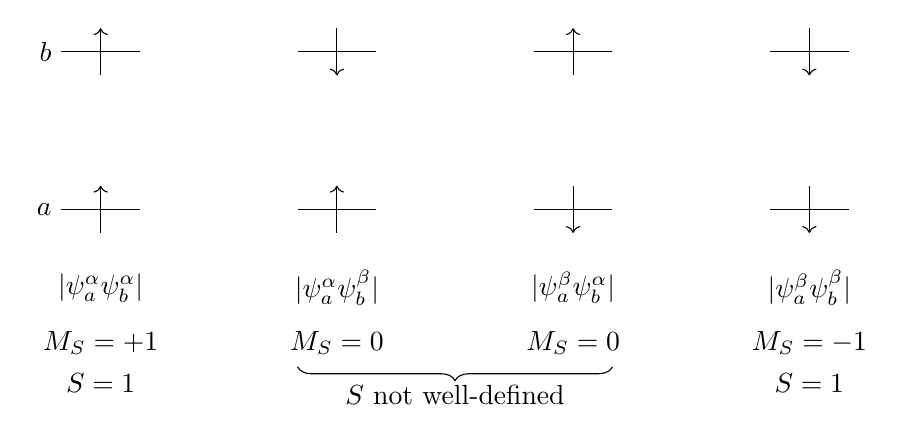
\begin{tikzpicture}
            \draw (0,0)node[left]{\(a\)}--(1,0);
            \draw (0,2)node[left]{\(b\)}--(1,2);
            \draw (3,0)--(4,0);
            \draw (3,2)--(4,2);
            \draw (6,0)--(7,0);
            \draw (6,2)--(7,2);
            \draw (9,0)--(10,0);
            \draw (9,2)--(10,2);
            \draw[->] (0.5,-0.3)--(0.5,0.3);
            \draw[->] (0.5,1.7)--(0.5,2.3);
            \draw[->] (3.5,-0.3)--(3.5,0.3);
            \draw[<-] (3.5,1.7)--(3.5,2.3);
            \draw[<-] (6.5,-0.3)--(6.5,0.3);
            \draw[->] (6.5,1.7)--(6.5,2.3);
            \draw[<-] (9.5,-0.3)--(9.5,0.3);
            \draw[<-] (9.5,1.7)--(9.5,2.3);
            \node at (0.5,-1) {\(|\psi_a^\alpha\psi_b^\alpha|\)};
            \node at (3.5,-1) {\(|\psi_a^\alpha\psi_b^\beta|\)};
            \node at (6.5,-1) {\(|\psi_a^\beta\psi_b^\alpha|\)};
            \node at (9.5,-1) {\(|\psi_a^\beta\psi_b^\beta|\)};
            \node at (0.5,-1.7) {\(M_S=+1\)};
            \node at (3.5,-1.7) {\(M_S=0\)};
            \node at (6.5,-1.7) {\(M_S=0\)};
            \node at (9.5,-1.7) {\(M_S=-1\)};
            \node at (0.5,-2.2) {\(S=1\)};
            \node at (9.5,-2.2) {\(S=1\)};
            \draw [decorate,decoration={brace,amplitude=5pt,mirror}] (3,-2) -- (7,-2) node[midway,yshift=-1em]{\(S\) not well-defined};
        \end{tikzpicture}
    \end{figure}

    The two states with \(M_S=+1\) and \(M_S=-1\) clearly must correspond to \(S=1\), but the \(S\) values of the two \(M_S=0\) states are not well defined. This is because these two Slater determinants cannot be factorised as a product of a spatial part and a spin part, so we can't assign the \(S\) value based on the symmetry of the spin part wavefunction (recall that the triplet \(S=1\) state has a symmetric spin wavefunction and the singlet \(S=0\) state has an antisymmetric wavefunction). On the other hand, e.g. the \(M_S=+1\) wavefunction can
    \begin{align}
        \abs{\psi_a^\alpha\psi_b^\alpha}&=\frac{1}{\sqrt{2}}[\psi_a(1)\alpha(1)\psi_b(2)\alpha(2)-\psi_b(1)\alpha(1)\psi_a(2)\alpha(2)]\notag\\
        &=\underbrace{\frac{1}{\sqrt{2}}[\psi_a(1)\psi_b(2)-\psi_b(1)\psi_a(2)]}_{\text{antisymmetric spatial wavefunction}}\quad\times \underbrace{\alpha(1)\alpha(2)}_{\text{symmetric spin wavefunction}}\,.
    \end{align}
    In fact, you will show in question sheet that the two \(M_S=0\) determinants above are linear combinations of the triplet \(M_S=0\) state and the singlet \(M_S=0\) states, so they are clearly not eigenfunctions of \(\hat{S}^2\).

    \subsubsection{More than Two Electrons}
    Our above calculations for systems with two electrons are already messy enough, and it will get even messier for more electrons. See \textit{B10: Electronic Structure} for details. However, the energy expression is in a very simple form
    \begin{equation}
        E=\sum_{i}h_{ii}+\sum_{i<j}\braket{ij}{ij}-\sum_{\begin{subarray}{c}
            i < j \\ \text{same spin}
        \end{subarray}}\braket{ij}{ji}+V^{\text{n-n}}\,.
    \end{equation}
    This should be reasonably physically intuitive --- we first sum over the one-electron energies, then each pair of electrons gives one Coulomb interaction, and each pair of electrons with the same spin gives one exchange integral.

    \begin{figure}[ht!]
        \centering
        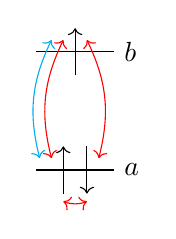
\begin{tikzpicture}
            \draw (0,0)--(1,0)node[right]{\(a\)};
            \draw (0,1.5)--(1,1.5)node[right]{\(b\)};
            \draw[->] (0.35,-0.3)--(0.35,0.3);
            \draw[<-] (0.65,-0.3)--(0.65,0.3);
            \draw[->] (0.5,1.2)--(0.5,1.8);
            \draw[<->,red] (0.35,-0.4) to[bend right=20] (0.65,-0.4);
            \draw[<->,red] (0.8,0.15) to[bend right=20] (0.65,1.65);
            \draw[<->,red] (0.2,0.15) to[bend left=20] (0.35,1.65);
            \draw[<->,cyan] (0.05,0.15) to[bend left=20] (0.2,1.65);
        \end{tikzpicture}
        \caption{A three-electron system. The red arrows are the Coulomb interactions and the blue arrows are the exchange interactions.}
    \end{figure}

    For example, the three electron system in the figure would have energy
    \begin{equation}
        E=2h_{aa}+h_{bb}+\braket{aa}{aa}+2\braket{ab}{ab}-\braket{ab}{ba}\,.
    \end{equation}

    \subsection{Hartree--Fock Theory}
    In the last section, we found an easy way of generating antisymmetric wavefunctions from orbitals using Slater determinants, and we have calculated the energies of these states. However, it seems that we have skipped the question of how to find these orbitals.

    Although H\"{u}ckel theory is a nice and easy way to do so, it actually misses a lot of things, such as the self-consistent interaction with the other electrons to get relative orbital energies correct. Instead, we will develop a method called the \textit{Hartree--Fock theory} (HF).

    Unlike H\"{u}ckel theory, which finds the stationary values of the orbital energies, the Hartree--Fock theory assumes the total wavefunction to be a single Slater determinant and it aims to minimise the total energy.

    Let's use ground state helium atom as an example, where the wavefunction is
    \begin{equation}
        \Psi=\frac{1}{\sqrt{2}}\abs{\psi_a^\alpha\psi_a^\beta}
    \end{equation}
    and the energy is
    \begin{equation}
        E=2h_{aa}+\braket{aa}{aa}\,.
    \end{equation}
    We want to find the \(\psi_a\) that minimises the total energy \(E\).    
    
    To express the wavefunction, we need some basis function. A sensible basis would be the hydrogenic orbitals of \(\mathrm{He^+}\), so we write
    \begin{equation}
        \psi_a=\sum_{i=1}^{n}c_i^{(a)}\phi_i\,,
    \end{equation}
    where \(\{\phi_i\}\) are the basis functions. Our problem now reduces to finding the coefficients \(c_i^{(a)}\) making the energy stationary. Let's take a closer look at the energy expression and write it more explicitly:
    \begin{equation}
        E=2\mel{\psi_a}{\hat{h}}{\psi_a}+\mel{\psi_a(1)\psi_a(2)}{\frac{1}{r_{12}}}{\psi_a(1)\psi_a(2)}\,.
    \end{equation}
    The one-electron term looks fine, but the two-electron (Coulomb) terms seem a bit complicated --- because it involves two electrons. We hope to simplify it to a one-electron integral, as electron 1 interacting with the average repulsion of electron 2. We have
    \begin{align}
        \mel{\psi_a(1)\psi_a(2)}{\frac{1}{r_{12}}}{\psi_a(1)\psi_a(2)}&=\int\dd[3]{\vb{r}_1}\dd[3]{\vb{r}_2}\frac{\psi_a^*(\vb{r}_1)\psi_a^*(\vb{r}_2)\psi_a(\vb{r}_1)\psi_a(\vb{r}_2)}{r_{12}}\notag\\
        &=\int\dd[3]{\vb{r}_1}\psi_a^*(\vb{r}_1)\left[\int\dd[3]{\vb{r}_2}\frac{\psi_a^*(\vb{r}_2)\psi_a(\vb{r}_2)}{r_{12}}\right]\psi_a(\vb{r}_1)\notag\\
        &=\int\dd[3]{\vb{r}_1}\psi_a^*(\vb{r}_1)\left[\hat{J}(\vb{r}_1)\right]\psi_a(\vb{r}_1)\,.
    \end{align}
    We defined a new operator, \(\hat{J}(\vb{r})\), the Coulomb operator. It is the potential energy an electron would receive on average due to Coulomb repulsion from the other electron.
    \begin{figure}
        \centering
        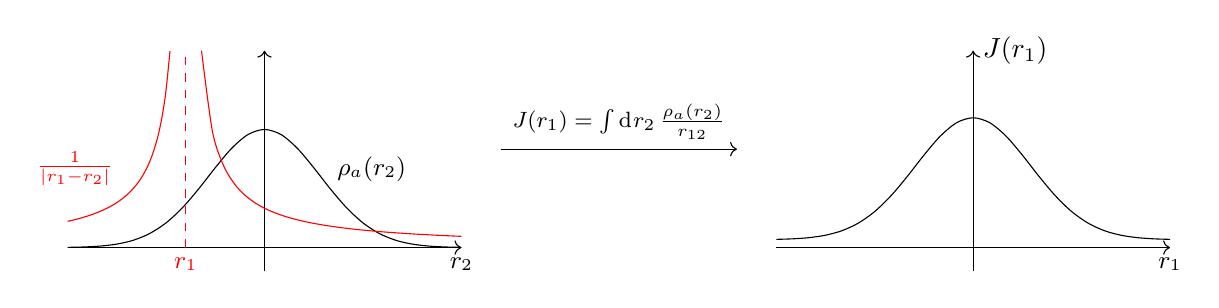
\begin{tikzpicture}
            \draw[->] (-2.5,0)--(2.5,0)node[below]{\small\(r_2\)};
            \draw[->] (0,-0.3)--(0,2.5);
            \node at (0.8,1)[right]{\small\(\rho_a(r_2)\)};
            \draw[domain=-2.5:2.5, smooth, variable=\x] plot ({\x}, {1.5*2.72^(-\x*\x)});
            \draw[domain=-1.5:-0.2, smooth, variable=\x,red] plot ({\x-1}, {-0.5/\x});
            \draw[domain=0.2:3.5, smooth, variable=\x,red] plot ({\x-1}, {0.5/\x});
            \node[red] at (-1.8,1)[left]{\small\(\frac{1}{\abs{r_1-r_2}}\)};
            \draw[dashed,red] (-1,0)node[below]{\small\(r_1\)}--(-1,2.5);
            \draw[->] (3,1.25)--node[above]{\footnotesize\(J(r_1)=\int\dd{r_2}\frac{\rho_a(r_2)}{r_{12}}\)}(6,1.25);
            \draw[->] (6.5,0)--(11.5,0)node[below]{\small\(r_1\)};
            \draw[->] (9,-0.3)--(9,2.5)node[right]{\(J(r_1)\)};
            \draw[domain=-2.5:2.5, smooth, variable=\x] plot ({\x+9}, {2.72^(-\x*\x)+0.3*2.72^(-(\x+0.3)*(\x+0.3))+0.3*2.72^(-(\x-0.3)*(\x-0.3))+0.1});
        \end{tikzpicture}
        \caption{An illustration of forming the Coulomb operator. At first glance it may seem that this integral diverges --- it does diverge in 1 dimension, but it nicely converges in 3 dimensions.}
    \end{figure}

    Therefore, we can write our total energy as
    \begin{equation}
        E=2\expval{\hat{h}}{\psi_a}+\expval{\hat{J}}{\psi_a}\,.
    \end{equation}
    We now need to find the \(\psi_a\) that minimises this. Again, the rigorous derivation is in course B10. We will illustrate everything briefly. Consider a variation \(\psi_a\to\psi_a+\delta\psi_a\). To meaningfully change \(\psi_a\), we require \(\braket{\delta\psi_a}{\psi_a}=0\). Then the variation in energy, to the first order, is
    \begin{equation}
        \delta E=4\mel{\delta\psi_a}{\hat{h}}{\psi_a}+4\mel{\delta\psi_a}{\hat{J}}{\psi_a}\,.
    \end{equation}
    This first order variation in energy vanishes at the minimum, which is satisfied when
    \begin{equation}
        [\hat{h}(\vb{r})+\hat{J}(\vb{r})]\psi_a(\vb{r})=\epsilon_a\psi_a(\vb{r})\,.
    \end{equation}
    We have therefore found a simple one-electron operator which takes into account electron-electron interactions. If we consider the more general case, with more electrons with different or same spins, we create what is known as the \textit{Fock operator},
    \begin{equation}
        \hat{F}(\vb{r})=\hat{h}(\vb{r})+\hat{J}(\vb{r})-\hat{K}(\vb{r})\,,
    \end{equation}
    where the \textit{Coulomb operator} \(\hat{J}\) accounts for the classical Coulomb repulsion between electrons, and \(\hat{K}\) is the \textit{exchange operator} which deals with exchange interactions, defined similarly as \(\hat{J}\).\footnote{More properly, \(\hat{J}\) includes the interaction with all electrons in the system, so \(\expval{\hat{J}}{\psi_a}\) actually includes the interaction of electron in orbital \(\psi_a\) with itself. This isn't a problem because this is exactly cancelled by an equal contribution in \(\hat{K}\) where the electron exchanges with itself. This is the cancellation of self-interaction, which only occurs if we treat exchange interaction exactly (as opposed to DFT).}

    The key result of these derivations is that we have created a new one-electron operator, the Fock operator, whose eigenfunctions are the molecular orbitals which minimise the energy of a Slater determinant. To find the orbitals we solve the \textit{Fock equations},
    \begin{equation}
        \hat{F}\psi_a=\epsilon_a\psi_a\,.
    \end{equation}
    Since we constructed the molecular orbitals by linear combination of atomic orbitals
    \begin{equation}
        \psi_a=\sum_i c_i^{(a)}\phi_i\,,
    \end{equation}
    we may solve the Fock equation in the matrix form. Define \textit{Fock matrix} \(F_{ij}=\mel{\phi_i}{\hat{F}}{\phi_j}\), the coefficients of the molecular orbitals are determined by the eigenvalue equation
    \begin{equation}
        \mathsf{F}\vb{c}^{(a)}=\epsilon_a\vb{c}^{(a)}\,.
    \end{equation}

    We may interpret \(\epsilon_a\) as the ``orbital energy'' of the orbital \(\psi_a\), but rigorously there is no such thing as ``orbital energy'' in Hartree--Fock theory --- there is only total energy. Moreover, it is absolutely wrong to obtain the total energy by adding up the orbital energies. It involves double-counting of interactions, just as what we discussed for H\"{u}ckel theory.

    \subsubsection{The Self-Consistent Field Procedure}
    Because the Fock operator, \(\hat{F}\) is both dependent on a set of orbitals (which are used to make \(\hat{J}\) and \(\hat{K}\)), and is used to define the orbitals, it is not entirely straightforward to actually solve the Fock equations to achieve orbitals which are eigenfunctions of their own Fock operator. The simplest way of doing this is to start with a guess set of orbitals and iterate until self-consistency, just as what we did in Kohn--Sham theory. This kind of method is known as \textit{self-consistent field} (SCF) method.\footnote{Since the Hartree--Fock theory is the first theory in quantum chemistry that uses a SCF procedure, Hartree--Fock theory itself is sometimes also referred to as the SCF method.} The general procedure goes as follows:
    \begin{enumerate}[topsep=0pt,label=(\roman*)]
        \item We first need to:
        \begin{enumerate}[topsep=0pt]
            \item[(a)] Specify the molecular geometry (coordinates of nuclei)
            \item[(b)] Specify the charge (the number of electrons)
            \item[(c)] Specify spin
            \item[(d)] Pick atomic orbital basis set 
        \end{enumerate}
        so that we know the form of the Hamiltonian and the Slater determinant \(\Psi=\frac{1}{\sqrt{n!}}\abs{\chi_1\chi_2\dots\chi_n}\).
        \item Make an initial guess of the orbitals for our system
        \begin{equation}
            \psi_n^{\text{guess}}=\sum_i c_i^{(n)}\phi_i
        \end{equation}
        using e.g. H\"{u}ckel theory.
        \item Work out the Fock operator and hence determine the Fock matrix in the atomic orbital basis
        \begin{equation}
            F_{ij}=\mel{\phi_i}{\hat{F}}{\phi_j}\,.
        \end{equation}
        \item Diagonalise \(\mathsf{F}\) to get the new molecular orbitals
        \begin{equation}
            \mathsf{F}\vb{c}^{(n)}=\epsilon_n\vb{c}^{(n)}\,.
        \end{equation}
        \item Compare the new \(\vb{c}^{(n)}\) to the previous \(\vb{c}^{(n)}\). If they are close enough (i.e. converged), then stop. Otherwise, go back to (iii).
        \item Calculate the total energy \(\expval{\hat{H}}{\Psi}\).
    \end{enumerate}

    \subsection{Electron Correlation}
    The key approximation in Hartree--Fock theory is the factorisation of the \(n\) electron wavefunction into one-electron orbitals. This is displayed in its most elementary form in equation (\ref{orbital_assumption}), and the Slater determinant form keeps this basic assumption while accounting for antisymmetrisation. In this product form it can be seen that the distribution of one electron is effectively independent from all the others --- their motion is not correlated with each other. In the true wavefunction, the singularity of the Coulomb interaction between electrons should give rise to a lowering of probability when they are close, and so this effect is missing in the Hartree product.

    Within a single Slater determinant, the antisymmetrisation does produce a Fermi hole around electrons of the same spin as the wavefunction vanishes when they are at the same point, so this approximation does take some correlation into account, but no such effect is present for electrons of opposite spin. This is observed by the fact that in both Hartree product form \(\Psi=\psi_1\psi_2\) and the singlet Slater determinant form \(\Psi=\frac{1}{\sqrt{2}}\abs{\psi_1^\alpha\psi_2^\beta}\), we have the probability of finding electrons at \(\vb{r}_1\) and \(\vb{r}_2\) to be
    \begin{equation}
        P(\vb{r}_1,\vb{r}_2)=\abs{\psi_1(\vb{r}_1)}^2\abs{\psi_2(\vb{r}_2)}^2\,.
    \end{equation}
    This lack of correlation is the origin of the error in the Hartree--Fock limit of equilibrium \(\mathrm{H_2}\).

    \begin{figure}
        \centering
        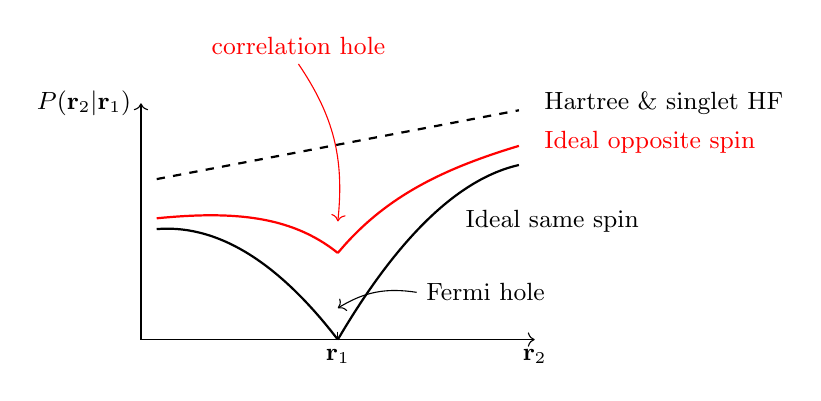
\begin{tikzpicture}
            \draw[->] (0,0)--(5,0)node[below]{\small\(\vb{r}_2\)};
            \draw[->] (0,0)--(0,3)node[left]{\small\(P(\vb{r}_2|\vb{r}_1)\)};
            \draw (2.5,0.1)--(2.5,0)node[below]{\small\(\vb{r}_1\)};
            \draw[domain=-2.3:0, smooth, variable=\x,thick] plot ({\x+2.5}, {-1.3*\x-0.3*\x*\x});
            \draw[domain=0:2.3, smooth, variable=\x,thick] plot ({\x+2.5}, {1.7*\x-0.32*\x*\x});
            \draw[domain=0.2:4.8, smooth, variable=\x,thick,dashed] plot ({\x}, {2+0.2*\x-0.01*\x});
            \draw[domain=-2.3:0, smooth, variable=\x,thick,red] plot ({\x+2.5}, {2.1+0.2*\x-2.72^\x});
            \draw[domain=0:2.3, smooth, variable=\x,thick,red] plot ({\x+2.5}, {2.1+0.2*\x-2.72^(-\x)});
            \node at (4,1.5)[right]{\small Ideal same spin};
            \node[red] at (5,2.5)[right]{\small Ideal opposite spin};
            \node at (5,3)[right]{\small Hartree \& singlet HF};
            \draw[->] (3.5,0.6)node[right]{\small Fermi hole} to[bend right=20] (2.5,0.4);
            \draw[->,red] (2,3.5)node[above]{\small correlation hole} to[bend left=20] (2.5,1.5);
        \end{tikzpicture}
        \caption{Dynamic correlation reduces the chances of electrons, even with the same spin, to approach.}
    \end{figure}

    The electron correlation error becomes more serious for stretched bonds, and grows to rather pathological proportions in the limit of full dissociation. The error in the dissociation limit can be quantified for \(\mathrm{H_2}\) by looking at the Hartree--Fock energy in the dissociated limit as \(R\to\infty\), which you will show in one exercise.
    \begin{equation}
        \lim_{R\to\infty}E_{\mathrm{H_2}}(R)=2E_{\mathrm{H}}+\frac{J_{\mathrm{H}}}{2}\,.
    \end{equation}
    We define the dissociation energy
    \begin{equation}
        \Delta_{\text{dissoc.}}=-\left(E_{\mathrm{H_2}}(R_{\text{eq}})-\lim_{R\to\infty}E_{\mathrm{H_2}}(R)\right)
    \end{equation}
    and the atomisation energy
    \begin{equation}
        \Delta_{\text{at.}}=-\left(E_{\mathrm{H_2}}(R_{\text{eq}})-2E_{\mathrm{H}}\right)\,.
    \end{equation}
    These energies should be the same, but they are not in HF theory --- Hartree--Fock theory over-predicts the dissociation energy by \(\frac{1}{2}J_{\mathrm{H}}\), which turns out to be about \(820\unit{kJ}\unit{mol}^{-1}\), a huge error.

    \begin{figure}
        \centering
        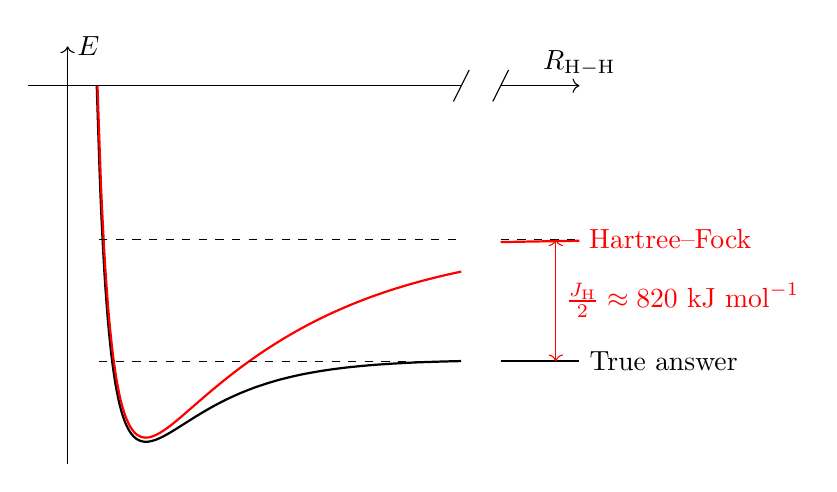
\begin{tikzpicture}
            \draw[domain=0.37:5, smooth, variable=\x,thick,samples=100] plot ({\x}, {1/(\x*\x)-5.5*2.72^(-\x)});
            \draw[domain=0.38:5, smooth, variable=\x,thick,red,samples=100] plot ({\x}, {1/(\x*\x)-5.5*2.72^(-0.5*\x)+1.55-0.5*2.72^(-\x*\x)});
            \draw[thick] (5.5,0)--(6.5,0)node[right]{True answer};
            \draw[domain=9.5:10.5, smooth, variable=\x,thick,red] plot ({\x-4}, {1/(\x*\x)-5.5*2.72^(-0.5*\x)+1.55-0.5*2.72^(-\x*\x)});
            \node[red] at (6.5,1.55)[right]{Hartree--Fock};
            \draw[dashed] (0.4,0)--(5,0);
            \draw[dashed] (0.4,1.55)--(5,1.55);
            \draw[dashed] (5.5,0)--(6.5,0);
            \draw[dashed] (5.5,1.55)--(6.5,1.55);
            \draw[<->,red] (6.2,0)--node[right]{\(\frac{J_{\mathrm{H}}}{2}\approx 820\unit{kJ}\unit{mol}^{-1}\)}(6.2,1.55);
            \draw[->] (0,-1.3)--(0,4)node[right]{\(E\)};
            \draw (-0.5,3.5)--(5,3.5);
            \draw (5.1,3.7)--(4.9,3.3);
            \draw (5.6,3.7)--(5.4,3.3);
            \draw[->] (5.5,3.5)--(6.5,3.5)node[above]{\(R_{\mathrm{H-H}}\)};
        \end{tikzpicture}
        \caption{The Hartree--Fock theory over-predicts the dissociation energy significantly due to the lack of correlation.}
    \end{figure}

    What's wrong with the Hartree--Fock solution? Let's have a look again at the ground-state wavefunction written as a product of molecular orbitals
    \begin{align}
        \Psi_{\text{HF}}(1,2)&=\frac{1}{\sqrt{2}}\begin{vmatrix}
            \psi_g^\alpha(1) & \psi_g^\beta(1) \\
            \psi_g^\alpha(2) & \psi_g^\beta(2)
        \end{vmatrix}\notag\\
        &=\frac{1}{2\sqrt{2}(1+S)}[\phi_a(1)+\phi_b(1)][\phi_a(2)+\phi_b(2)][\alpha(1)\beta(2)-\beta(1)\alpha(2)]\,,
    \end{align}
    where \(S=\braket{\phi_a}{\phi_b}\) is the overlap integral. Expanding the product over the spatial orbitals, after omitting the spin orbitals which will not affect the final energy, we get
    \begin{equation}\label{H2_HF_expand}
        \Psi_{\text{HF}}(1,2)\sim\underbrace{\phi_a(1)\phi_a(2)}_{\text{ionic}}+\underbrace{\phi_a(1)\phi_b(2)}_{\text{bi-radical}}+\underbrace{\phi_b(1)\phi_a(2)}_{\text{bi-radical}}+\underbrace{\phi_b(1)\phi_b(2)}_{\text{ionic}}\,.
    \end{equation}
    We may interpret the terms as either ionic, with both electrons on one of the hydrogens, and a bare nucleus as the other, or bi-radical, with each hydrogen getting a single electron. Because of these ionic terms, the Hartree--Fock wavefunction cannot properly describe molecular dissociation (which should not contain the ionic terms in this limit).

    \begin{figure}
        \centering
        \begin{tikzpicture}
            \draw (0,0)--(1,0)node[right]{\(\psi_g\)};
            \draw (0,1.6)--(1,1.6)node[right]{\(\psi_u\)};
            \draw (3.3,0) circle (0.3);
            \draw (2.7,0) circle (0.3);
            \draw (3.3,1.6) circle (0.3);
            \draw[fill=gray!30] (2.7,1.6) circle (0.3);
            \draw[->] (0.4,-0.3)--(0.4,0.3);
            \draw[<-] (0.6,-0.3)--(0.6,0.3);
            \draw[->] (4.5,1.3)--(6,2.3);
            \draw[->] (4.5,0.3)--(6,-0.7);
            \draw (7,2.3)--(8,2.3)node[right]{\(\phi_a\)};
            \draw (7,-0.7)--(8,-0.7)node[right]{\(\phi_a\)};
            \draw (9,2.3)--(10,2.3)node[right]{\(\phi_b\)};
            \draw (9,-0.7)--(10,-0.7)node[right]{\(\phi_b\)};
            \draw[dashed] (7.9,-1.5)node[left]{\(\mathrm{H}^{\vdot}\)}--(9.5,-1.5)node[right]{\(\mathrm{H}^{\vdot}\)};
            \draw[->] (7.5,-1)--(7.5,-0.4);
            \draw[<-] (9.5,-1)--(9.5,-0.4);
            \node at (11,-0.7)[right]{bi-radical};
            \draw[dashed] (7.9,1.5)node[left]{\(\mathrm{H}^{-}\)}--(9.5,1.5)node[right]{\(\mathrm{H}^{+}\)};
            \draw[->] (7.4,2)--(7.4,2.6);
            \draw[<-] (7.6,2)--(7.6,2.6);
            \node at (11,2.3)[right]{ionic};
        \end{tikzpicture}
        \caption{Due to the lack of electron correlation, Hartree--Fock predicts a dissociation into a superposition of bi-radical and ionic states. We can view this as two \(\frac{1}{2}\)-electrons are attached to each atom at dissociation.}
    \end{figure}

    Recall that Hartree--Fock arises from an approximation, and although \(\Psi_{\text{HF}}\) is the best possible single determinant which can describe our molecule, it is not an eigenfunction of the many-electron Hamiltonian. (This is because the orbitals in HF are eigenfunctions of the Fock operators, while the total Hamiltonian is not a sum of the Fock operators.) With this single-determinant approach, the electrons are effectively independent of each other and the probability distributions of electrons are independent. At dissociation this is very problematic, as we know the correct wavefunction
    has one electron on each atom.

    In the exact wavefunction at dissociation, the probability of finding both electrons around the same nucleus is therefore very small indeed, but in this Hartree--Fock wavefunction it is \(50\%\). In order to improve the description of molecular dissociation, one must introduce electron correlation, such that if one electron finds itself around one nucleus, the other electron has an enhanced probability of finding itself around the other nucleus.

    \subsubsection{Configuration Interaction}
    How can one introduce such electron correlation? One approach is to go beyond the use of a single Slater determinant to represent the wavefunction, and use a linear combination of multiple Slater determinants. For example, for the two-electron case, we may write the wavefunction as
    \begin{equation}
        \Psi(1,2)=\Psi_0+\sum_I c_I\Psi_I\,,
    \end{equation}
    where \(\Psi_0\) is the ground state Slater determinant (Hartree--Fock solution) and \(\Psi_I\) are the Slater determinants with further excitations. This wavefunction \(\Psi\) is known as a \textit{multi-determinantal wavefunction}. We can find the best possible coefficients \(c_I\) by variational principles. This method of introducing electron correlation is called \textit{configuration interaction}.

    \begin{figure}[ht!]
        \centering
        \begin{tikzpicture}
            \draw (0,0)node[left]{\(\psi_g\)}--(1,0);
            \draw (0,1.6)node[left]{\(\psi_u\)}--(1,1.6);
            \draw[->] (0.4,-0.3)--(0.4,0.3);
            \draw[<-] (0.6,-0.3)--(0.6,0.3);
            \node at (0.5,-0.8){\(\Psi_0\)};

            \draw (3,0)node[left]{\(\psi_g\)}--(4,0);
            \draw (3,1.6)node[left]{\(\psi_u\)}--(4,1.6);
            \draw[->] (3.4,1.3)--(3.4,2);
            \draw[<-] (3.6,1.3)--(3.6,2);
            \node at (3.5,-0.8){\(\Psi_2\)};
        \end{tikzpicture}
    \end{figure}

    Why is the introduction of excitation states helpful? Let's consider the \(\mathrm{H_2}\) molecule again. It turns out that it will be particularly useful to introduce a second determinant with doubly occupied anti-bonding orbital \(\psi_u=\frac{1}{\sqrt{2(1-S)}}(\phi_a-\phi_b)\)
    \begin{align}
        \Psi_2(1,2)&=\frac{1}{\sqrt{2}}\begin{vmatrix}
            \psi_u^\alpha(1) & \psi_u^\beta(1)\\
            \psi_u^\alpha(2) & \psi_u^\beta(2)
        \end{vmatrix}\notag\\
        &=\frac{1}{2\sqrt{2}(1-S)}[\phi_a(1)-\phi_b(1)][\phi_a(2)-\phi_b(2)][\alpha(1)\beta(2)-\beta(1)\alpha(2)]\notag\\
        &\sim\underbrace{\phi_a(1)\phi_a(2)}_{\text{ionic}}-\underbrace{\phi_a(1)\phi_b(2)}_{\text{bi-radical}}-\underbrace{\phi_b(1)\phi_a(2)}_{\text{bi-radical}}+\underbrace{\phi_b(1)\phi_b(2)}_{\text{ionic}}\,.
    \end{align}
    We call this \(\Psi_2\) because we denote the Hartree--Fock ground state \(\Psi_0\) and we preserve \(\Psi_1\) for the singly excited state. Notice that in \(\Psi_2\) the ionic components of the wavefunction come with the opposite sign to the bi-radical parts. Therefore if we subtract \(\Psi_2\) from \(\Psi_0\) (the Hartree--Fock solution (\ref{H2_HF_expand})) we remove the troublesome ionic factors, leaving
    \begin{equation}
        c_0\Psi_0-c_2\Psi_2\sim[\phi_a(1)\phi_b(2)+\phi_b(1)\phi_a(2)][\alpha(1)\beta(2)-\beta(1)\alpha(2)]\,,
    \end{equation}
    which dissociates correctly.

    How do we solve for the coefficients of each Slater determinant in the configuration interaction? The answer is to use the variational principle. Define the Hamiltonian matrix in the basis of the Slater determinants \(H_{IJ}=\mel{\Psi_I}{\hat{H}}{\Psi_J}\). Since the orbitals are orthonormal (as they are the eigenstates of the Fock operator), so too are the Slater determinants. The secular equation we need to solve is
    \begin{equation}
        (\mathsf{H}-E_A\mathsf{I})\vb{c}^{(A)}=\vb{0}\,.
    \end{equation}
    The coefficients and energies are the eigenvalues and eigenvectors of \(\mathsf{H}\).

    Back to our \(\mathrm{H_2}\) case, the secular equation is
    \begin{equation}
        \begin{pmatrix}
            E_0-E & U \\
            U & E_2-E
        \end{pmatrix}=0\,,
    \end{equation}
    where \(E_0=H_{00}, E_2=H_{22}, U=H_{02}=H_{20}\). The solutions are
    \begin{equation}
        E=\frac{E_0+E_2}{2}\pm\frac{1}{2}\sqrt{(E_0-E_2)^2+4U^2}\,.
    \end{equation}
    In the limit of small \(U\) at large \(R\), we have
    \begin{equation}
        E_0^{(\text{CI})}\approx E_0+\frac{U^2}{E_0-E_2}\quad\text{and}\quad E_2^{(\text{CI})}\approx E_2-\frac{U^2}{E_0-E_2}\,,
    \end{equation}
    and similarly one can show that
    \begin{equation}
        \Psi_0^{(\text{CI})}\approx\Psi_0+\frac{U}{E_0-E_2}\Psi_2\,.
    \end{equation}

    \begin{figure}
        \centering
        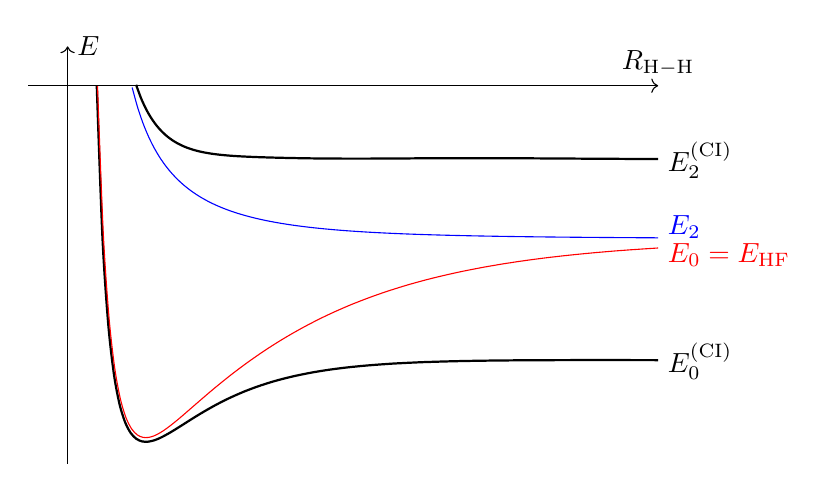
\begin{tikzpicture}
            \draw[domain=0.37:7.5, smooth, variable=\x,thick,samples=100] plot ({\x}, {1/(\x*\x)-5.5*2.72^(-\x)});
            \draw[domain=0.38:7.5, smooth, variable=\x,red,samples=100] plot ({\x}, {1/(\x*\x)-5.5*2.72^(-0.5*\x)+1.55-0.5*2.72^(-\x*\x)});
            \draw[domain=0.82:7.5, smooth, variable=\x,blue,samples=100] plot ({\x}, {1/(\x*\x)+2.72^(-\x)+1.55});
            \draw[domain=0.87:7.5, smooth, variable=\x,thick,samples=100] plot ({\x}, {1/(\x*\x)+2.72^(-\x)+2.55-2.72^(-0.35*\x*\x)-0.02*\x*\x*\x*2.72^(-0.2*\x*\x)});
            \draw[->] (0,-1.3)--(0,4)node[right]{\(E\)};
            \draw[->] (-0.5,3.5)--(7.5,3.5)node[above]{\(R_{\mathrm{H-H}}\)};
            \node at (7.5,0)[right]{\(E_0^{(\text{CI})}\)};
            \node[red] at (7.5,1.35)[right]{\(E_0=E_{\text{HF}}\)};
            \node[blue] at (7.5,1.7)[right]{\(E_2\)};
            \node at (7.5,2.55)[right]{\(E_2^{(\text{CI})}\)};
        \end{tikzpicture}
        \caption{We can retain some of the electron correlation by configuration interaction.}
    \end{figure}

    One can further improve the wavefunction by enlarging the basis and constructing other (indeed all) possible excited determinants which have the same symmetry and spin (\(^1\Sigma_g^+\)) as \(\Psi_0\). The limit of including all determinants it is possible to make with a given set of orbitals is known as \textit{Full CI}, and is the best possible answer given our choice of basis set (the atomic orbitals). This provides, in principle, a systematic technique to introduce correlation. However, it is not in general a practical method, because the number of possible excited-state determinants grows in a factorial (i.e. exponential) manner (both with number of basis functions and the number of electrons). Methods to treat accurately electron correlation remain one of the most active and challenging areas of Theoretical Chemistry.

    \subsubsection{Wavefunction-based Methods of Correlation}
    We have seen that for even a simple molecule like \(\mathrm{H_2}\), there is a rich complexity to its wavefunction, and a technique like Hartree--Fock theory is not able to exactly reproduce the binding-curve --- a treatment of electron correlation is essential. If the Full CI limit is computationally feasible we should use it, but in practice it can be used only for the very smallest systems because of the exponentially large size of Slater determinant space.
    
    An appealing option would be to simply truncate the determinant space, including Slater determinants which differ by at most \(x\) electrons from the Hartree--Fock determinant; \(x\) is known as the excitation level. Unfortunately, performing CI in this naively truncated space leads to wavefunctions whose quality becomes significantly worse as the system size studied increases (because the \(x\)-excitation configuration takes a smaller and smaller proportion of the full CI as the number of electrons increases) so this is not a generally useful method.

    All is not lost, however, and there exist two systematically improvable methods which are routinely used in electronic structure. \textit{M{\o}ller--Plesset} (MP) Theory and \textit{coupled cluster} (CC) Theory. They will be covered in the \textit{B10: Electronic Structure} course, but key to their use is that they each form a family of methods where you can go to a more accurate level to be sure that you are sufficiently converged. M{\o}ller--Plesset methods are based on perturbation theory and labelled MP2,\dots,MP\(n\) where \(n\) labels the level of perturbation theory (see also the \textit{C7: Further Quantum Mechanics} course). Coupled Cluster methods are labelled with the level of excitation which is explicitly treated in the wavefunction: CCSD, CCSDT, CCSDTQ,\dots\ These differ from truncated CI methods in that quality of the energies for a given truncation level does not worsen as the system size increases. Hybrids of these methods exist where the final level of excitation is treated perturbatively, denoted: CCSD(T), CCSDT(Q),\dots\ These are routinely used as they have a lower computational scaling than the full method and produce extremely good approximations to the equivalent full CC method.

    \renewcommand{\arraystretch}{1}
    \begin{table}
        \centering
        \begin{tabular}{cccc}
            \toprule
            \multirow{2}{*}{Method} & \multirow{2}{*}{Scaling} & Bond length & Atomisation energy \\
            ~ & ~ & Error / \(\!\unit{pm}\) & Error / \(\!\unit{kJ}\unit{mol}^{-1}\) \\ \midrule
            HF & \(N^3\) & 2.7 & 423 \\
            MP2 & \(N^5\) & 0.5 & 36 \\
            MP3 & \(N^6\) & 1.2 & ~ \\
            MP4 & \(N^7\) & 0.4 & ~ \\
            MP\(n\) & \(N^{n+3}\) & ~ & ~ \\
            CCSD & \(N^6\) & 0.8 & 37 \\
            CCSDT & \(N^8\) & 0.1 & 3 \\
            CC\dots\(x\) & \(N^{2x+2}\) & ~ & ~ \\
            CCSD(T) & \(N^7\) & 0.2 & 5 \\ \midrule
            Experiment & ~ & 0.2 & 4 \\ \midrule
            Approx. value & ~ & 150 & 1500 \\ \bottomrule
        \end{tabular}
        \caption{The typical errors of different \textit{ab initio} methods. CCSD(T) is seen as the golden standard of quantum chemistry.}
    \end{table}

    \section{Reaction Theory}
    Most chemical reactions involve a change in the distribution of electrons, and the journey from reactants to products usually encounters some form of barrier on the potential energy surface. To understand the origin of these barriers we will consider how the multiple electronic states of a molecule change along a reaction pathway. Before this, however, we will consider again the initial assumptions that went into decoupling the nuclear and electronic wavefunctions in the Born--Oppenheimer approximation,
    \begin{equation}
        \Psi_{\text{BO}}(\mathsf{r},\mathsf{R})=\Psi_{e}(\mathsf{r};\mathsf{R})\Psi_n(\mathsf{R})\,.
    \end{equation}

    \subsection{Beyond the Born--Oppenheimer Approximation (Not Lectured)}
    The question arises, how good is the Born--Oppenheimer approximation, and when does it break down? To analyse this, we must consider a slightly more complicated form of the total wavefunction. Recall that there are in fact many solutions of the electronic Schrödinger equation, each corresponding to different electronic states, which we label \(k\); these have energies \(E_{e}^{(k)}(\mathsf{R})\) and wavefunctions \(\Psi_{e}^{(k)}(\mathsf{r};\mathsf{R})\). The lowest electronic state, which has \(k=0\), corresponds to the very lowest energy configuration of electrons in the system for each nuclear state, as if the electrons were allowed to relax completely at each geometry. The electronic eigenfunctions are known as the \textit{adiabatic electronic states}.\footnote{In this context, a system being \textit{adiabatic} means that the conditions are only changing gradually such that the system is allowed to adapt its configuration. Hence the Born--Oppenheimer approximation is also known as the \textit{adiabatic approximation}. We assume that the electronic motion is faster than the nuclear motion, and for each nuclear geometry, the electrons are in their ground state. This is an example of the adiabatic theorem, which states that a physical system remains in its instantaneous eigenstate if a given perturbation is acting on it slowly enough and if there is a gap between the eigenvalue and the rest of the Hamiltonian's spectrum.}

    To each electronic state, we can associate a nuclear wavefunction \(\Psi_n^{(k)}(\mathsf{R})\), which could be obtained by solving the nuclear Schr\"{o}dinger equation. To a first approximation, one could consider each state to be independent, but quantum mechanics has a nasty habit of coupling things together, and so to solve for the correct wavefunctions we must write the total wavefunction as a superposition of these states. Our first guess might take the form
    \begin{equation}
        \Psi_{\text{total}}(\mathsf{r},\mathsf{R})=\sum_k C_k\Psi_e^{(k)}(\mathsf{r};\mathsf{R})\Psi_n^{(k)}(\mathsf{R})\,,
    \end{equation}
    which linearly combines the electronic states each with its own nuclear wavefunction. Though there are many solutions to the Schr\"{o}dinger equation of this form, we are concerned with the total wavefunction with the lowest total energy. We see that the Born--Oppenheimer approximation amounts to taking a single term in this sum, and is sometimes called the \textit{adiabatic approximation}. For most chemical purposes, the Born--Oppenheimer approximation proves sufficient, but to achieve spectroscopically accurate energies, additional corrections must be taken into account, though these are generally less than \(1\unit{kJ}\unit{mol}^{-1}\) in magnitude.

    \subsection{Avoided Crossing and Conical Intersections}
    Whilst the electronic states which are eigenfunctions of the electronic Schr\"{o}dinger equation are convenient, they are not always so easy to interpret, as to minimise the energy the nature of the electronic state may change rapidly. An example of this is the dissociation of the diatomic \(\mathrm{LiF}\). In its ground equilibrium electronic state, it occurs mostly as \(\mathrm{Li^+ F^-}\), but by comparing ionization energies and electron affinities we conclude that at infinite separation this molecule should separate into neutral fragments, \(\mathrm{Li}^{\vdot}\) and \(\mathrm{F}^{\vdot}\).\footnote{The ionisation energy of \(\mathrm{Li}\) is \(520\unit{kJ}\unit{mol}^{-1}\) and the electron affinity of \(\mathrm{F}\) is \(320\unit{kJ}\unit{mol}^{-1}\), i.e.
    \begin{align*}
        \mathrm{Li}\,& \mathrm{\longrightarrow Li^+ + e^-} & &520\unit{kJ}\unit{mol}^{-1}\\
        \mathrm{F^-}\,& \mathrm{\longrightarrow F + e^-} & &320\unit{kJ}\unit{mol}^{-1}\,.
    \end{align*}
    In fact, any diatomics would dissociate to atoms because all ionisation energies are larger than electron affinities.} A chemically intuitive view is to consider these two different pictures as different electronic states. These are known as \textit{diabatic states}, loosely defined as the states where the nature of the electronic state changes less quickly as the geometry changes. The diabatic states are not electronic eigenfunctions, and provide an alternative representation to the adiabatic electronic states. For most purposes they can be regarded as an interpretative tool.

    \begin{figure}
        \centering
        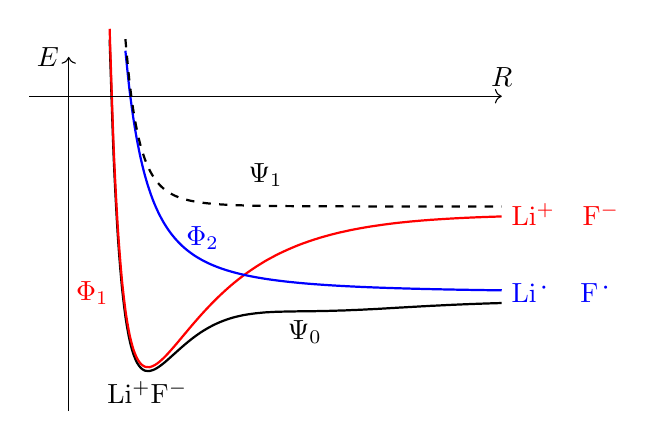
\begin{tikzpicture}
            \draw[domain=0.52:5.5, smooth, variable=\x,thick,samples=100] plot ({\x}, {1/(\x*\x*\x)-8*2.72^(-\x)-1.1+1.05*2.72^(-0.38*(\x-1)*(\x-1))});
            \draw[domain=0.52:5.5, smooth, variable=\x,red,samples=100,thick] plot ({\x}, {1/(\x*\x*\x)-8*2.72^(-\x)});
            \draw[domain=0.72:5.5, smooth, variable=\x,blue,samples=100,thick] plot ({\x}, {1/((\x-0.15)*(\x-0.15))-1});
            \draw[domain=0.72:5.5, smooth, variable=\x,thick,samples=100,dashed] plot ({\x}, {1/((\x+0.14)^5)+0.1});
            \draw[->] (0,-2.5)--(0,2)node[left]{\(E\)};
            \draw[->] (-0.5,1.5)--(5.5,1.5)node[above]{\(R\)};
            \node at (1,-2)[below]{\(\mathrm{Li^+ F^-}\)};
            \node at (3,-1.5){\(\Psi_0\)};
            \node at (2.5,0.5){\(\Psi_1\)};
            \node[red] at (0.3,-1){\(\Phi_1\)};
            \node[blue] at (1.7,-0.3){\(\Phi_2\)};
            \node[blue] at (5.5,-1)[right]{\(\mathrm{Li^{\vdot}\quad F^{\vdot}}\)};
            \node[red] at (5.5,0)[right]{\(\mathrm{Li^{+}\quad F^{-}}\)};
        \end{tikzpicture}
        \caption{\(\Phi_1,\Phi_2\) are \textit{diabatic states}, where electrons do not respond to the nuclei. \(\Psi_0,\Psi_1\) are \textit{adiabatic states} where we allow electrons to relax at each nuclear position. When the ground state \(\Psi_0\) \(\mathrm{LiF}\) dissociates as \(R\) increases, it changes from predominantly \(\Phi_1\) to \(\Phi_1\pm\Phi_2\) (sign depends on \(\mel{\Phi_1}{\hat{H}}{\Phi_2}\)) then to \(\Phi_2\).}
    \end{figure}

    In \(\mathrm{LiF}\), we see that the ionic state will have a considerably higher energy than the bi-radical state at dissociation, and so the two diabatic states will cross somewhere along the dissociation curve. Recalling that the diabatic states are not electronic eigenfunctions, we may ask the following question: What combination of the diabatic states will give us the lowest energy? Calling these states \(\Phi_1\) and \(\Phi_2\), we see that we can simply solve the secular equations in this basis, and diagonalize \(H_{ij}=\mel{\Phi_i}{\hat{H}}{\Phi_{j}}\). The ground state of this will be a linear combination of the two diabatic states with the lowest energy --- the adiabatic state.

    If the states are widely separated in energy (\(\abs{H_{11}-H_{22}}\gg 0\)) the lowest of these will be a good approximation to the adiabatic state. When \(\abs{H_{11}-H_{22}}\approx 0\), however, we must consider role of the off-diagonal element \(H_{12}\). This controls the mixing of the two diabatic states, and if it is non-zero, then when these states are close in energy, the adiabatic state will become an approximately equal mix of the two, smoothly changing from one to the other, splitting the two states apart. This effect is known as an \textit{avoided crossing}. In general, unless there are symmetry reasons, \(H_{12}\) will not be zero, and so all such crossings will be avoided and the adiabatic ground state will not intersect with the excited state. This is rigorously true for diatomics, but for higher dimensional systems, there exist points of \textit{accidental degeneracy} where \(H_{11}=H_{22}\) and \(H_{12}=0\). These crossing points are known as \textit{conical intersections} and have a dramatic effect on the excited electronic states of the molecule (especially on their relaxation). They are beyond the scope of this course.

    \begin{figure}
        \centering
        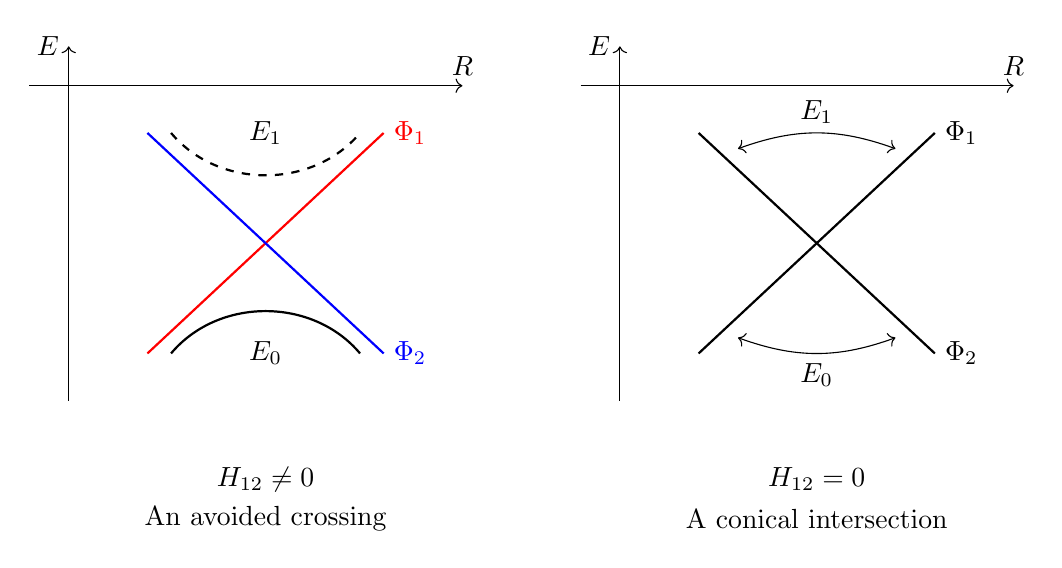
\begin{tikzpicture}
            \draw[->] (-0.5,4)--(5,4)node[above]{\(R\)};
            \draw[->] (0,0)--(0,4.5)node[left]{\(E\)};
            \draw[thick, red] (1,0.6)--(4,3.4)node[right]{\(\Phi_1\)};
            \draw[thick, blue] (1,3.4)--(4,0.6)node[right]{\(\Phi_2\)};
            \draw[thick] (1.3,0.6) to[bend left=50] (3.7,0.6);
            \draw[thick,dashed] (1.3,3.4) to[bend right=50] (3.7,3.4);
            \node at (2.5,0.6) {\(E_0\)};
            \node at (2.5,3.4) {\(E_1\)};
            \node at (2.5,-1) {\(H_{12}\ne 0\)};
            \node at (2.5,-1.5) {An avoided crossing};

            \draw[->] (6.5,4)--(12,4)node[above]{\(R\)};
            \draw[->] (7,0)--(7,4.5)node[left]{\(E\)};
            \draw[thick] (8,0.6)--(11,3.4)node[right]{\(\Phi_1\)};
            \draw[thick] (8,3.4)--(11,0.6)node[right]{\(\Phi_2\)};
            \draw[<->] (8.5,0.8) to[bend right=20] node[below]{\(E_0\)} (10.5,0.8);
            \draw[<->] (8.5,3.2) to[bend left=20] node[above]{\(E_1\)} (10.5,3.2);
            \node at (9.5,-1) {\(H_{12}= 0\)};
            \node at (9.5,-1.5) {A conical intersection};
        \end{tikzpicture}
        \caption{Normally when two diabatic states cross, there will be an avoided crossing. A conical intersection will occur when \(H_{12}=0\) for symmetry reasons or occasionally accidentally.}
    \end{figure}

    \subsection{Chemical Reactions}
    In this section, we will apply what we previously discussed to predict whether a reaction would be feasible or not. We will use pericyclic reactions as examples. Look at the two reactions in the figure. Reaction (a) is the [4+2] (Diels--Alder) cycloaddition, and it occurs readily, whereas the corresponding [2+2] reaction is forbidden. Why should this be? Presumably, the latter reaction encounters a substantial barrier which is not present in the former --- can the presence or absence of large barriers be understood solely in terms of the underlying MOs?

    \begin{figure}
        \centering
        \begin{tikzpicture}
            \node at (0,0){
                \schemestart[][west]
                    \chemfig{=_[:150]-[:90]=_[:30]}
                    \quad\arrow{0}[,0]\+\arrow{0}[,0]\quad
                    \chemfig{=[:90]}
                    \arrow{->}
                    \chemfig{*6(-----=)}
                \schemestop
            };
            \node at (7,0){
                \schemestart[][west]
                    \chemfig{=[:90]}
                    \quad \arrow{0}[,0]\+\arrow{0}[,0]\,
                    \chemfig{=[:90]}
                    \arrow{->}
                    \chemfig{*4(----)}
                \schemestop
            };
            \node at (0,-2) {(a)};
            \node at (7,-2) {(b)};
        \end{tikzpicture}
        \caption{(a) The [4+2] Diels--Alder cycloaddition; (b) a [2+2] forbidden cycloaddition}
    \end{figure}

    \subsubsection{Orbital Correlation Diagrams}
    During a chemical reaction, we can parameterise the progress of the reaction by a \textit{reaction coordinate}, along which the geometry of the system evolves smoothly from the reactants to the products. We want to track how the electronic structure of the system evolves as we move along the reaction coordinate. From now on, we will assume the wavefunctions of each molecule in the reactants and the products can be well-represented by a single Slater determinant. At the start and end, the electronic structure is determined by the MOs of the reactants and products respectively. We may trace the diabatic states along the reaction coordinate by considering Slater determinants made from specific occupations of these orbitals; along the reaction coordinate the orbitals will adapt to the new geometry, but the occupancy of the orbitals remains constant for a given diabatic state.

    Along the reaction coordinate the molecular orbitals can, in principle, be calculated at every point, but in practice we only care about the energy ordering of the orbitals so can we may approximate how the orbitals change along the reaction by lines which join the orbitals of the reactants and the orbitals of the product. Crucially, orbitals of the same symmetry cannot cross in energy.

    In general, to construct an orbital correlation diagram, we follow the following steps:
    \begin{enumerate}[topsep=0pt,label=(\roman*)]
        \item Specify the reactants and the products.
        \item Find a symmetry (the point group) during the whole reaction process.
        \item Draw energy-ordered MOs of the reactants and products. Occupied orbitals corresponding to bonds which do not change can be ignored.
        \item Draw the energy levels for each MO (in products and reactants) and label them with the conserved symmetry.
        \item Working up the diagram from the lowest energy, for each orbital on the left, connect it to the lowest not-yet-connected orbital of the same symmetry on the right. Lines corresponding to orbitals of the same symmetry should not cross.
    \end{enumerate}

    \begin{figure}
        \centering
        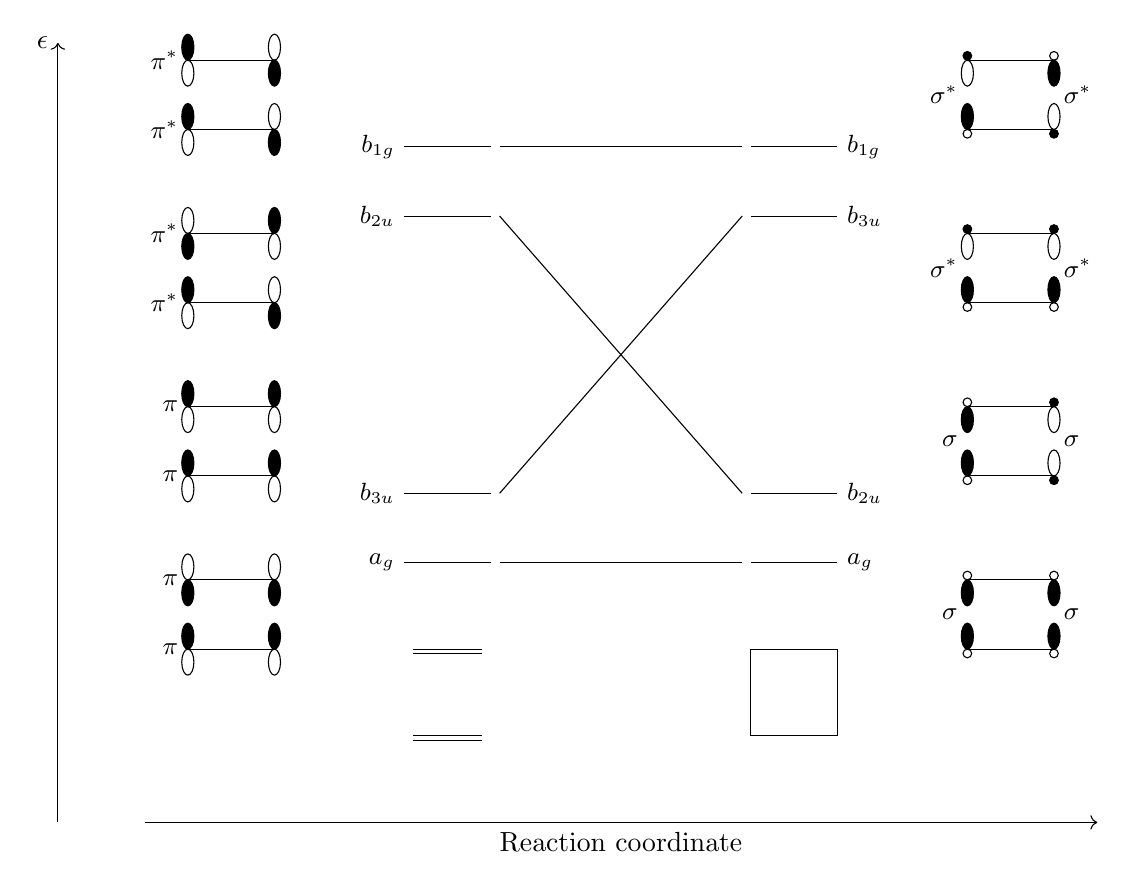
\begin{tikzpicture}[scale=1.1]
            \draw (0,0)node[left]{\small\(a_g\)}--(1,0);
            \draw (0,0.8)node[left]{\small\(b_{3u}\)}--(1,0.8);
            \draw (0,4)node[left]{\small\(b_{2u}\)}--(1,4);
            \draw (0,4.8)node[left]{\small\(b_{1g}\)}--(1,4.8);

            \draw (-2.5,-0.2)node[left]{\small\(\pi\)}--(-1.5,-0.2);
            \draw (-2.5,-1)node[left]{\small\(\pi\)}--(-1.5,-1);
            \draw (-2.5,-0.05) ellipse (0.07cm and 0.15 cm);
            \draw (-1.5,-0.05) ellipse (0.07cm and 0.15 cm);
            \draw[fill=black] (-2.5,-0.35) ellipse (0.07cm and 0.15 cm);
            \draw[fill=black] (-1.5,-0.35) ellipse (0.07cm and 0.15 cm);
            \draw[fill=black] (-2.5,-0.85) ellipse (0.07cm and 0.15 cm);
            \draw[fill=black] (-1.5,-0.85) ellipse (0.07cm and 0.15 cm);
            \draw (-2.5,-1.15) ellipse (0.07cm and 0.15 cm);
            \draw (-1.5,-1.15) ellipse (0.07cm and 0.15 cm);

            \draw (-2.5,1)node[left]{\small\(\pi\)}--(-1.5,1);
            \draw (-2.5,1.8)node[left]{\small\(\pi\)}--(-1.5,1.8);
            \draw[fill=black] (-2.5,1.95) ellipse (0.07cm and 0.15 cm);
            \draw[fill=black] (-1.5,1.95) ellipse (0.07cm and 0.15 cm);
            \draw (-2.5,1.65) ellipse (0.07cm and 0.15 cm);
            \draw (-1.5,1.65) ellipse (0.07cm and 0.15 cm);
            \draw[fill=black] (-2.5,1.15) ellipse (0.07cm and 0.15 cm);
            \draw[fill=black] (-1.5,1.15) ellipse (0.07cm and 0.15 cm);
            \draw (-2.5,0.85) ellipse (0.07cm and 0.15 cm);
            \draw (-1.5,0.85) ellipse (0.07cm and 0.15 cm);

            \draw (-2.5,3.8)node[left]{\small\(\pi^*\)}--(-1.5,3.8);
            \draw (-2.5,3)node[left]{\small\(\pi^*\)}--(-1.5,3);
            \draw (-2.5,3.95) ellipse (0.07cm and 0.15 cm);
            \draw[fill=black] (-1.5,3.95) ellipse (0.07cm and 0.15 cm);
            \draw[fill=black] (-2.5,3.65) ellipse (0.07cm and 0.15 cm);
            \draw (-1.5,3.65) ellipse (0.07cm and 0.15 cm);
            \draw[fill=black] (-2.5,3.15) ellipse (0.07cm and 0.15 cm);
            \draw (-1.5,3.15) ellipse (0.07cm and 0.15 cm);
            \draw (-2.5,2.85) ellipse (0.07cm and 0.15 cm);
            \draw[fill=black] (-1.5,2.85) ellipse (0.07cm and 0.15 cm);

            \draw (-2.5,5)node[left]{\small\(\pi^*\)}--(-1.5,5);
            \draw (-2.5,5.8)node[left]{\small\(\pi^*\)}--(-1.5,5.8);
            \draw[fill=black] (-2.5,5.95) ellipse (0.07cm and 0.15 cm);
            \draw (-1.5,5.95) ellipse (0.07cm and 0.15 cm);
            \draw (-2.5,5.65) ellipse (0.07cm and 0.15 cm);
            \draw[fill=black] (-1.5,5.65) ellipse (0.07cm and 0.15 cm);
            \draw[fill=black] (-2.5,5.15) ellipse (0.07cm and 0.15 cm);
            \draw (-1.5,5.15) ellipse (0.07cm and 0.15 cm);
            \draw (-2.5,4.85) ellipse (0.07cm and 0.15 cm);
            \draw[fill=black] (-1.5,4.85) ellipse (0.07cm and 0.15 cm);




            \draw (4,0)--(5,0)node[right]{\small\(a_g\)};
            \draw (4,0.8)--(5,0.8)node[right]{\small\(b_{2u}\)};
            \draw (4,4)--(5,4)node[right]{\small\(b_{3u}\)};
            \draw (4,4.8)--(5,4.8)node[right]{\small\(b_{1g}\)};

            \draw (0.1,-1)--(0.9,-1);
            \draw (0.1,-1.05)--(0.9,-1.05);
            \draw (0.1,-2)--(0.9,-2);
            \draw (0.1,-2.05)--(0.9,-2.05);

            \draw (4,-1)--(5,-1)--(5,-2)--(4,-2)--(4,-1);

            \draw (6.5,-0.2)--(7.5,-0.2);
            \draw (6.5,-1)--(7.5,-1);
            \draw (6.5,-0.15) circle (0.05);
            \draw (7.5,-0.15) circle (0.05);
            \draw[fill=black] (6.5,-0.35) ellipse (0.07cm and 0.15 cm);
            \draw[fill=black] (7.5,-0.35) ellipse (0.07cm and 0.15 cm);
            \draw[fill=black] (6.5,-0.85) ellipse (0.07cm and 0.15 cm);
            \draw[fill=black] (7.5,-0.85) ellipse (0.07cm and 0.15 cm);
            \draw (6.5,-1.05) circle (0.05);
            \draw (7.5,-1.05) circle (0.05);
            \node at (6.5,-0.6)[left]{\small\(\sigma\)};
            \node at (7.5,-0.6)[right]{\small\(\sigma\)};

            \draw (6.5,1)--(7.5,1);
            \draw (6.5,1.8)--(7.5,1.8);
            \draw (6.5,1.85) circle (0.05);
            \draw[fill=black] (7.5,1.85) circle (0.05);
            \draw[fill=black] (6.5,1.65) ellipse (0.07cm and 0.15 cm);
            \draw (7.5,1.65) ellipse (0.07cm and 0.15 cm);
            \draw[fill=black] (6.5,1.15) ellipse (0.07cm and 0.15 cm);
            \draw (7.5,1.15) ellipse (0.07cm and 0.15 cm);
            \draw (6.5,0.95) circle (0.05);
            \draw[fill=black] (7.5,0.95) circle (0.05);
            \node at (6.5,1.4)[left]{\small\(\sigma\)};
            \node at (7.5,1.4)[right]{\small\(\sigma\)};

            \draw (6.5,3.8)--(7.5,3.8);
            \draw (6.5,3)--(7.5,3);
            \draw[fill=black] (6.5,3.85) circle (0.05);
            \draw[fill=black] (7.5,3.85) circle (0.05);
            \draw (6.5,3.65) ellipse (0.07cm and 0.15 cm);
            \draw (7.5,3.65) ellipse (0.07cm and 0.15 cm);
            \draw[fill=black] (6.5,3.15) ellipse (0.07cm and 0.15 cm);
            \draw[fill=black] (7.5,3.15) ellipse (0.07cm and 0.15 cm);
            \draw (6.5,2.95) circle (0.05);
            \draw (7.5,2.95) circle (0.05);
            \node at (6.5,3.4)[left]{\small\(\sigma^*\)};
            \node at (7.5,3.4)[right]{\small\(\sigma^*\)};

            \draw (6.5,5)--(7.5,5);
            \draw (6.5,5.8)--(7.5,5.8);
            \draw[fill=black] (6.5,5.85) circle (0.05);
            \draw (7.5,5.85) circle (0.05);
            \draw (6.5,5.65) ellipse (0.07cm and 0.15 cm);
            \draw[fill=black] (7.5,5.65) ellipse (0.07cm and 0.15 cm);
            \draw[fill=black] (6.5,5.15) ellipse (0.07cm and 0.15 cm);
            \draw (7.5,5.15) ellipse (0.07cm and 0.15 cm);
            \draw (6.5,4.95) circle (0.05);
            \draw[fill=black] (7.5,4.95) circle (0.05);
            \node at (6.5,5.4)[left]{\small\(\sigma^*\)};
            \node at (7.5,5.4)[right]{\small\(\sigma^*\)};

            \draw[->] (-3,-3)--node[below]{Reaction coordinate}(8,-3);
            \draw[->] (-4,-3)--(-4,6)node[left]{\(\epsilon\)};
            \draw (1.1,0)--(3.9,0);
            \draw (1.1,0.8)--(3.9,4);
            \draw (1.1,4)--(3.9,0.8);
            \draw (1.1,4.8)--(3.9,4.8);
            
        \end{tikzpicture}
        \caption{The orbital correlation diagram for ethene dimerisation.}
        \label{ethene_correlation}
    \end{figure}

    As an example, let us first consider the [2+2] system in \cref{ethene_correlation}. The unreacted ethene molecules have two sets of \(\pi\)-orbitals, whereas the cyclobutane product has two newly-formed \(\sigma\)-orbitals. In the unreacted state, the ground-state configuration is \((a_g)^2(b_{3u})^2\). If the electrons maintain in their original orbitals, then this will eventually lead to a doubly excited state in the product. Even if this double occupancy is not maintained all the way, but just to the transition state (approximately midway on the diagram), the energy of the system is substantially higher than the initial state. As a result, the reaction is forbidden if the starting molecule is in the ground state. On the other hand, if the molecule is photo-excited initially, promoting an electron from \(b_{3u}\) to \(b_{2u}\), the reaction proceeds without an unduly large barrier. This reaction is photo-active.

    \begin{figure}
        \centering
        \begin{tikzpicture}[scale=1.2]
            \draw[->] (0,-0.5)--(0,4)node[left]{\(\epsilon\)};
            \draw (1,0)node[left]{\small\(a_g\)}--(1.8,0);
            \draw (1,0.5)node[left]{\small\(b_{3u}\)}--(1.8,0.5);
            \draw (1,3)node[left]{\small\(b_{2u}\)}--(1.8,3);
            \draw (1,3.5)node[left]{\small\(b_{1g}\)}--(1.8,3.5);

            \draw (4,0)--(4.8,0)node[right]{\small\(a_g\)};
            \draw (4,0.5)--(4.8,0.5)node[right]{\small\(b_{2u}\)};
            \draw (4,3)--(4.8,3)node[right]{\small\(b_{3u}\)};
            \draw (4,3.5)--(4.8,3.5)node[right]{\small\(b_{1g}\)};
            \draw (1.9,0)--(3.9,0);
            \draw (1.9,0.5)--(3.9,3);
            \draw (1.9,3)--(3.9,0.5);
            \draw (1.9,3.5)--(3.9,3.5);
            \draw[->] (1.35,-0.2)--(1.35,0.2);
            \draw[<-] (1.45,-0.2)--(1.45,0.2);
            \draw[->] (1.35,0.3)--(1.35,0.7);
            \draw[<-] (1.45,0.3)--(1.45,0.7);
            \draw[->] (4.35,-0.2)--(4.35,0.2);
            \draw[<-] (4.45,-0.2)--(4.45,0.2);
            \draw[->] (4.35,2.8)--(4.35,3.2);
            \draw[<-] (4.45,2.8)--(4.45,3.2);

            \draw[->] (7,-0.5)--(7,4)node[left]{\(\epsilon\)};
            \draw (8,0)node[left]{\small\(a_g\)}--(8.8,0);
            \draw (8,0.5)node[left]{\small\(b_{3u}\)}--(8.8,0.5);
            \draw (8,3)node[left]{\small\(b_{2u}\)}--(8.8,3);
            \draw (8,3.5)node[left]{\small\(b_{1g}\)}--(8.8,3.5);

            \draw (11,0)--(11.8,0)node[right]{\small\(a_g\)};
            \draw (11,0.5)--(11.8,0.5)node[right]{\small\(b_{2u}\)};
            \draw (11,3)--(11.8,3)node[right]{\small\(b_{3u}\)};
            \draw (11,3.5)--(11.8,3.5)node[right]{\small\(b_{1g}\)};
            \draw (8.9,0)--(10.9,0);
            \draw (8.9,0.5)--(10.9,3);
            \draw (8.9,3)--(10.9,0.5);
            \draw (8.9,3.5)--(10.9,3.5);
            \draw[->] (8.35,-0.2)--(8.35,0.2);
            \draw[<-] (8.45,-0.2)--(8.45,0.2);
            \draw[->] (8.4,0.3)--(8.4,0.7);
            \draw[<-] (8.4,2.8)--(8.4,3.2);
            \draw[->] (11.35,-0.2)--(11.35,0.2);
            \draw[->] (11.45,-0.2)--(11.45,0.2);
            \draw[<-] (11.4,0.3)--(11.4,0.7);
            \draw[->] (11.4,2.8)--(11.4,3.2);
        \end{tikzpicture}
        \caption{The reaction is forbidden if the reactant is in the electronic ground state. However this reaction is photo-active.}
    \end{figure}

    \subsubsection{State Correlation Diagram}
    The situation will be clearer by introducing the \textit{state correlation diagram}. This is similar to the orbital correlation diagram, but we are correlating the electronic states between the reactants and the products. Again, there will be avoided crossing when two states with the same symmetry intersects.

    In practice, we will consider only the ground electronic state and the first few excited states, and the states they corresponds to in the product. For our cycloaddition, we will consider
    \begin{align}
        \text{Ground state }&\Phi_0\quad (A_g):\quad \ a_g^2b_{3u}^2 \\
        \text{Singly excited }&\Phi_1\quad (B_{1g}):\quad a_g^2b_{3u}^1b_{2u}^1 \\
        \text{Doubly excited }&\Phi_2\quad (A_g): \quad \ a_g^2b_{2u}^2\,.
    \end{align}

    \begin{figure}
        \centering
        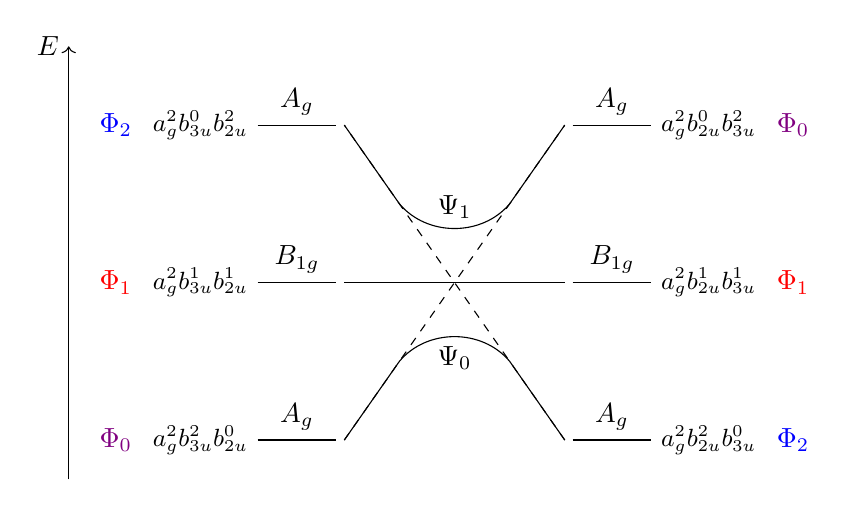
\begin{tikzpicture}
            \draw[->] (-2.4,-0.5)--(-2.4,5)node[left]{\(E\)};
            \draw (0,0)node[left]{\small \(a_g^2b_{3u}^2b_{2u}^0\)}--node[above]{\(A_g\)}(1,0);
            \draw (0,2)node[left]{\small \(a_g^2b_{3u}^1b_{2u}^1\)}--node[above]{\(B_{1g}\)}(1,2);
            \draw (0,4)node[left]{\small \(a_g^2b_{3u}^0b_{2u}^2\)}--node[above]{\(A_g\)}(1,4);
            \node[violet] at (-1.8,0){\(\Phi_0\)};
            \node[red] at (-1.8,2){\(\Phi_1\)};
            \node[blue] at (-1.8,4){\(\Phi_2\)};

            \draw (4,0)--node[above]{\(A_g\)}(5,0)node[right]{\small \(a_g^2b_{2u}^2b_{3u}^0\)};
            \draw (4,2)--node[above]{\(B_{1g}\)}(5,2)node[right]{\small \(a_g^2b_{2u}^1b_{3u}^1\)};
            \draw (4,4)--node[above]{\(A_g\)}(5,4)node[right]{\small \(a_g^2b_{2u}^0b_{3u}^2\)};
            \node[violet] at (6.8,4){\(\Phi_0\)};
            \node[red] at (6.8,2){\(\Phi_1\)};
            \node[blue] at (6.8,0){\(\Phi_2\)};
            \draw[dashed] (1.1,0)--(3.9,4);
            \draw[dashed] (3.9,0)--(1.1,4);
            \draw (1.1,2)--(3.9,2);
            \draw (1.1,0)--(1.8,1.0) to[bend left=50] node[below]{\(\Psi_0\)}(3.2,1.0)--(3.9,0);
            \draw (1.1,4)--(1.8,3) to[bend right=50] node[above]{\(\Psi_1\)} (3.2,3)--(3.9,4);
        \end{tikzpicture}
        \caption{The state correlation diagram for ethene dimerisation. There is a high energy barrier so the reaction is thermally forbidden.}
    \end{figure}

    Since the ground state and the doubly-excited state are of the same symmetry, they can mix, and do so quite substantially as they become energetically close. The energy and the coefficients of \(\Psi_i\) in terms of \(\Phi_i\) can be obtained by solving secular equations. If we let
    \begin{equation}
        \begin{aligned}
            E_0&=\expval{\hat{H}}{\Phi_0}\\
            E_2&=\expval{\hat{H}}{\Phi_2}\\
            U&=\mel{\Phi_0}{\hat{H}}{\Phi_2}\,,
        \end{aligned}
    \end{equation}
    then solving
    \begin{equation}
        \begin{vmatrix}
            E_0-E & U \\
            U & E_2-E
        \end{vmatrix}=0
    \end{equation}
    gives
    \begin{equation}
        E=\frac{E_0+E_2}{2}\pm\frac{1}{2}\sqrt{(E_0-E_2)^2+4U^2}\approx E_0\pm\frac{U^2}{E_0-E_2}
    \end{equation}
    in the \(\abs{U}\ll\abs{E_0-E_2}\) limit.

    It appears as if the two states repel each other, irrespective of the sign of \(U\); the ground-state is lowered in energy and the excited state pushed up. This is the basis for the non-crossing rule for states with the same symmetry. The first excited state, being of a different symmetry, is unaffected. The magnitude of the repulsion depends both on \(U\) and on the energy difference of the two diabatic states. At the transition state, the energy difference is small and so the `repulsion' is greatest.

    Nevertheless, even with the above lowering of energy, there remains a large barrier (compared to the thermal energy available to the molecules) to reaction for the ground-state, and ethene dimerisation remains therefore thermally forbidden.

    Turning now to the [4+2] cycloaddition. We notice that only a \(\sigma\) symmetry is preserved during the process, so we label everything under the \(C_s\) point group symmetry. Using the same process as before, we can see from the state correlation diagram that there is no energy barrier for the transitions of the electronic ground states between the reactants and the product, so the reaction is thermally allowed.

    \begin{figure}
        \centering
        \includegraphics[width=0.6\textwidth]{DA_orbital_corr.png}
        \caption{The orbital correlation diagrams for the Diels--Alder reaction. Figure adapted from the official course notes by Dr. Alex Thom.}
    \end{figure}

    \begin{figure}
        \centering
        \begin{tikzpicture}[scale=1.6]
            \draw[->] (-1,-0.5)--(-1,6)node[left]{\(\epsilon\)};
            \foreach \i in {0,...,5}{
                \draw (0,0.12*\i)--(1,0.12*\i);
                \draw (0,2.5+0.12*\i)--(1,2.5+0.12*\i);
                \draw (0,5+0.12*\i)--(1,5+0.12*\i);
            }
            \foreach \i in {0,1,2}{
                \draw (5,0.48+0.12*\i)--(6,0.48+0.12*\i);
                \draw (5,0.12-0.12*\i)--(6,0.12-0.12*\i);
                \draw (5,2.98+0.12*\i)--(6,2.98+0.12*\i);
                \draw (5,2.62-0.12*\i)--(6,2.62-0.12*\i);
                \draw (5,5.48+0.12*\i)--(6,5.48+0.12*\i);
                \draw (5,5.12-0.12*\i)--(6,5.12-0.12*\i);
            }
            \draw[-{Classical TikZ Rightarrow[length=0.7mm]}] (0.15,-0.1)--(0.15,0.1);
            \draw[{Classical TikZ Rightarrow[length=0.7mm]}-] (0.25,-0.1)--(0.25,0.1);
            \draw[-{Classical TikZ Rightarrow[length=0.7mm]}] (0.45,0.02)--(0.45,0.22);
            \draw[{Classical TikZ Rightarrow[length=0.7mm]}-] (0.55,0.02)--(0.55,0.22);
            \draw[-{Classical TikZ Rightarrow[length=0.7mm]}] (0.75,0.14)--(0.75,0.34);
            \draw[{Classical TikZ Rightarrow[length=0.7mm]}-] (0.85,0.14)--(0.85,0.34);

            \draw[-{Classical TikZ Rightarrow[length=0.7mm]}] (0.15,2.4)--(0.15,2.6);
            \draw[{Classical TikZ Rightarrow[length=0.7mm]}-] (0.25,2.4)--(0.25,2.6);
            \draw[-{Classical TikZ Rightarrow[length=0.7mm]}] (0.45,2.52)--(0.45,2.72);
            \draw[{Classical TikZ Rightarrow[length=0.7mm]}-] (0.55,2.52)--(0.55,2.72);
            \draw[-{Classical TikZ Rightarrow[length=0.7mm]}] (0.8,2.64)--(0.8,2.84);
            \draw[{Classical TikZ Rightarrow[length=0.7mm]}-] (0.5,2.76)--(0.5,2.96);

            \draw[-{Classical TikZ Rightarrow[length=0.7mm]}] (0.15,4.9)--(0.15,5.1);
            \draw[{Classical TikZ Rightarrow[length=0.7mm]}-] (0.25,4.9)--(0.25,5.1);
            \draw[-{Classical TikZ Rightarrow[length=0.7mm]}] (0.5,5.02)--(0.5,5.22);
            \draw[{Classical TikZ Rightarrow[length=0.7mm]}-] (0.5,5.38)--(0.5,5.58);
            \draw[-{Classical TikZ Rightarrow[length=0.7mm]}] (0.75,5.14)--(0.75,5.34);
            \draw[{Classical TikZ Rightarrow[length=0.7mm]}-] (0.85,5.14)--(0.85,5.34);

            \draw[-{Classical TikZ Rightarrow[length=0.7mm]}] (5.15,-0.22)--(5.15,-0.02);
            \draw[{Classical TikZ Rightarrow[length=0.7mm]}-] (5.25,-0.22)--(5.25,-0.02);
            \draw[-{Classical TikZ Rightarrow[length=0.7mm]}] (5.45,-0.10)--(5.45,0.10);
            \draw[{Classical TikZ Rightarrow[length=0.7mm]}-] (5.55,-0.10)--(5.55,0.10);
            \draw[-{Classical TikZ Rightarrow[length=0.7mm]}] (5.75,0.02)--(5.75,0.22);
            \draw[{Classical TikZ Rightarrow[length=0.7mm]}-] (5.85,0.02)--(5.85,0.22);

            \draw[-{Classical TikZ Rightarrow[length=0.7mm]}] (5.15,2.28)--(5.15,2.48);
            \draw[{Classical TikZ Rightarrow[length=0.7mm]}-] (5.25,2.28)--(5.25,2.48);
            \draw[-{Classical TikZ Rightarrow[length=0.7mm]}] (5.45,2.4)--(5.45,2.6);
            \draw[{Classical TikZ Rightarrow[length=0.7mm]}-] (5.55,2.4)--(5.55,2.6);
            \draw[-{Classical TikZ Rightarrow[length=0.7mm]}] (5.8,2.52)--(5.8,2.72);
            \draw[{Classical TikZ Rightarrow[length=0.7mm]}-] (5.5,2.88)--(5.5,3.08);

            \draw[-{Classical TikZ Rightarrow[length=0.7mm]}] (5.15,4.78)--(5.15,4.98);
            \draw[{Classical TikZ Rightarrow[length=0.7mm]}-] (5.25,4.78)--(5.25,4.98);
            \draw[-{Classical TikZ Rightarrow[length=0.7mm]}] (5.5,4.9)--(5.5,5.1);
            \draw[{Classical TikZ Rightarrow[length=0.7mm]}-] (5.5,5.5)--(5.5,5.7);
            \draw[-{Classical TikZ Rightarrow[length=0.7mm]}] (5.75,5.02)--(5.75,5.22);
            \draw[{Classical TikZ Rightarrow[length=0.7mm]}-] (5.85,5.02)--(5.85,5.22);

            \node at (0,0.3)[left] {\(A\)};
            \node at (0,2.8)[left] {\(A'\)};
            \node at (0,5.3)[left] {\(A'\)};
            \node at (6,0.3)[right] {\(A\)};
            \node at (6,2.8)[right] {\(A'\)};
            \node at (6,5.3)[right] {\(A'\)};

            \draw (1.3,0.3)--(2,0.3);
            \draw (1.3,2.8)--(2,2.8);
            \draw (1.3,5.3)--(2,5.3);
            \draw (4,0.3)--(4.7,0.3);
            \draw (4,2.8)--(4.7,2.8);
            \draw (4,5.3)--(4.7,5.3);
            \draw (2.1,0.3)--(3.9,0.3);
            \draw[dashed] (2.1,2.8)--(3.9,5.3);
            \draw[dashed] (2.1,5.3)--(3.9,2.8);
            \draw (2.1,2.8)--(2.55,3.425)to[bend left=50](3.45,3.425)--(3.9,2.8);
            \draw (2.1,5.3)--(2.55,4.675)to[bend right=50](3.45,4.675)--(3.9,5.3);
        \end{tikzpicture}
        \caption{The state correlation diagram of the Diels--Alder reaction. The reaction of the ground state is thermally allowed.}
    \end{figure}

    Similar considerations work for ring-opening and ring-closing, where different mechanisms, called \textit{con-rotatory} and \textit{dis-rotatory} can be allowed or forbidden, which leads to methods for selective synthesis of cis- or trans- products. You will investigate this in one of the exercises. These symmetry considerations are codified more generally in the \textit{Woodward--Hoffmann rules} which you may encounter in the further study of pericyclic reactions.

\end{document}